%!TEX root = ../Thesis.tex
%% Basierend auf TeXnicCenter-Vorlage von Mark Müller
%%                      Willi Nüßer
%%                      Waldemar Penner     
%%                      Ulrich Reus
%%                      Frank Plass
%%                      Oliver Tribeß 
%%                      Daniel Hintze     
%%%%%%%%%%%%%%%%%%%%%%%%%%%%%%%%%%%%%%%%%%%%%%%%%%%%%%%%%%%%%%%%%%%%%%%

% Wählen Sie die Optionen aus, indem Sie % vor der Option entfernen  
% Dokumentation des KOMA-Script-Packets: scrguide

%%%%%%%%%%%%%%%%%%%%%%%%%%%%%%%%%%%%%%%%%%%%%%%%%%%%%%%%%%%%%%%%%%%%%%%
%% Optionen zum Layout des Artikels                                  %%
%%%%%%%%%%%%%%%%%%%%%%%%%%%%%%%%%%%%%%%%%%%%%%%%%%%%%%%%%%%%%%%%%%%%%%%
\documentclass[%
paper=A4,         % alle weiteren Papierformat einstellbar
fontsize=12pt,    % Schriftgröße (12pt, 11pt (Standard))
BCOR12mm,         % Bindekorrektur, bspw. 1 cm
DIV14,            % breiter Satzspiegel
%parskip=half*,    % Absatzformatierung s. scrguide 3.1
headsepline,      % Trennline zum Seitenkopf  
%footsepline,     % Trennline zum Seitenfuß
%normalheadings,  % Überschriften etwas kleiner (smallheadings)
listof=totoc,     % Tabellen & Abbildungsverzeichnis ins Inhaltsverzeichnis      
%bibtotoc,        % Literaturverzeichnis im Inhalt 
%draft            % Überlangen Zeilen in Ausgabe gekennzeichnet
footinclude=false,% Fußzeile in die Satzspiegelberechnung einbeziehen 
headinclude=true, % Kopfzeile in die Satzspiegelberechnung einbeziehen 
final             % draft beschleunigt die Kompilierung
]
{scrartcl}

\usepackage{parskip}

%\setuptoc{toc}{totoc} % Inhaltsverzeichnis ins Inhaltsverzeichnis

% Neue Deutsche Rechtschreibung und Deutsche Standardtexte
\usepackage[ngerman]{babel} 

% Umlaute können verwendet werden
\usepackage[utf8]{inputenc}   

% Echte Umlaute
\usepackage[T1]{fontenc} 

% Latin Modern Font, Type1-Schriftart für nicht-englische Texte
\usepackage{lmodern} 

% 1/2-zeiliger Zeilenabstand
\usepackage[onehalfspacing]{setspace}

% Für die Defenition eigener Kopf- und Fußzeilen
\usepackage{fancyhdr} 

% Für die Verwendung von Grafiken
\usepackage[pdftex]{graphicx}

% Bessere Tabellen
\usepackage{tabularx}

% Für die Befehle \toprule, \midrule und \bottomrule, z.B. in Tabellen 
\usepackage{booktabs}

% Erlaubt die Benutzung von Farben
\usepackage{color}

% Verbessertes URL-Handling mit \url{http://...}
\usepackage{url}

% Listen ohne Abstände \begin{compactlist}...\end{compactlist}
\usepackage{paralist} 

% Ausgabe der aktuellen Uhrzeit für die Draft-Versionen
\usepackage{datetime}

% Deutsche Anführungszeichen
\usepackage[babel,german=quotes]{csquotes}

% Konfiguration der Abbildungs- und Tabellenbezeichnungen
\usepackage[format=hang, font={footnotesize, sf}, labelfont=bf, justification=raggedright,singlelinecheck=false]{caption}

% Verbessert die Lesbarkeit durch Mikrotypografie
\usepackage[activate={true,nocompatibility},final,tracking=true,kerning=true,spacing=true,factor=1100,stretch=10,shrink=10]{microtype}  

% Zitate und Quellenverzeichnis
\usepackage[
    bibstyle=authoryear,
    citestyle=authoryear-fhdw,  
    firstinits=false,         % false = Vornamen werden ausgeschrieben
    natbib=true,
    urldate=long,             % "besucht am" - Datum
    %url=false,
    date=long,                
    dashed=false, 
    maxcitenames=3,           % max. Anzahl Autorennamen in Zitaten
    maxbibnames=99,           % max. Anzahl Autorennamen im Quellenverzeichnis
    %backend=bibtex           % Ggf. für ältere Distributionen bibtex verwenden
    backend=biber
]{biblatex}
  
% Bibliograpthy
\bibliography{library/library}

% Ebenentiefe der Nummerierung
\setcounter{secnumdepth}{3}

% Gliederungstiefe im Inhaltsverzeichnis 
\setcounter{tocdepth}{3} 

% Tabellen- und Abbildungsverzeichnis mit Bezeichnung:
\usepackage[titles]{tocloft}

% Sourcecode-Listings
\usepackage{listings}

% Bestimmte Warnungen unterdrücken
% siehe http://tex.stackexchange.com/questions/51867/koma-warning-about-toc
\usepackage{scrhack} 

%% http://tex.stackexchange.com/questions/126839/how-to-add-a-colon-after-listing-label
\makeatletter
\begingroup\let\newcounter\@gobble\let\setcounter\@gobbletwo
  \globaldefs\@ne \let\c@loldepth\@ne
  \newlistof{listings}{lol}{\lstlistlistingname}
\endgroup
\let\l@lstlisting\l@listings
\makeatother

\renewcommand*\cftfigpresnum{Abbildung~}
\renewcommand*\cfttabpresnum{Tabelle~}
\renewcommand*\cftlistingspresnum{Listing~}
\renewcommand{\cftfigaftersnum}{:}
\renewcommand{\cfttabaftersnum}{:}
\renewcommand{\cftlistingsaftersnum}{:}
\settowidth{\cftfignumwidth}{\cftfigpresnum 99~\cftfigaftersnum}
\settowidth{\cfttabnumwidth}{\cfttabpresnum 99~\cftfigaftersnum}
\settowidth{\cftlistingsnumwidth}{\cftlistingspresnum 99~\cftfigaftersnum}
\setlength{\cfttabindent}{1.5em}
\setlength{\cftfigindent}{1.5em}
\setlength{\cftlistingsindent}{1.5em}

\renewcommand\lstlistlistingname{Listingverzeichnis}
 
% Style für Kopf- und Fußzeilenfelder
\pagestyle{fancy}
\fancyhf{}
\fancyhead[R]{\leftmark}
\fancyfoot[R]{\thepage} 
\renewcommand{\sectionmark}[1]{\markboth{#1}{#1}} 
\fancypagestyle{plain}{}

% Macro für Quellenangaben unter Abbildungen und Tabellen
\newcommand{\source}[1]{{\vspace{-1mm}\\\footnotesize\textsf{\textbf{Quelle:}} \textsf{#1}\par}}

% Anpassungen der Formatierung an Eclipse-Aussehen 
% http://jevopi.blogspot.de/2010/03/nicely-formatted-listings-in-latex-with.html
%\definecolor{sh_comment}{rgb}{0.12, 0.38, 0.18 } %adjusted, in Eclipse: {0.25, 0.42, 0.30 } = #3F6A4D
%\definecolor{sh_keyword}{rgb}{0.37, 0.08, 0.25}  % #5F1441
%\definecolor{sh_string}{rgb}{0.06, 0.10, 0.98} % #101AF9
% Für Druckausgabe sollte alles schwarz sein
\definecolor{sh_comment}{rgb}{0.0, 0.0, 0.0 }
\definecolor{sh_keyword}{rgb}{0.0, 0.0, 0.0 }
\definecolor{sh_string}{rgb}{0.0, 0.0, 0.0 }

\lstset{ %
  language=Java,
  basicstyle=\small\ttfamily,
  fontadjust, 
  xrightmargin=1mm,
  xleftmargin=5mm,
  tabsize=2,
  columns=flexible,
  showstringspaces=false,
  rulesepcolor=\color{black},
  showspaces=false,showtabs=false,tabsize=2,
  stringstyle=\color{sh_string},
  keywordstyle=\color{sh_keyword}\bfseries,
  commentstyle=\color{sh_comment}\itshape,
  captionpos=t,
  lineskip=-0.3em
}

%\makeatletter
%\def\l@lstlisting#1#2{\@dottedtocline{1}{0em}{1.5em}{\lstlistingname\space{#1}}{#2}}
%\makeatother

% Anhangsverzeichnis
\usepackage[nohints]{minitoc} %Anhangsverzeichnis

\makeatletter
\newcounter{fktnr}\setcounter{fktnr}{0}
\newcounter{subfktnr}[fktnr]\setcounter{subfktnr}{0}

\renewcommand\thesubfktnr{\arabic{fktnr}.\arabic{subfktnr}}
\newcounter{anhangcounter}
\newcommand{\blatt}{\stepcounter{anhangcounter}}

\newcommand{\anhang}[1]{\setcounter{anhangcounter}{0}\refstepcounter{fktnr}
\addcontentsline{fk}{subsection}{Anhang~\thefktnr: \hspace*{1em}#1}
\subsection*{{Anhang~\thefktnr \hspace*{1em} #1 \hspace*{-1em}}}
}

\newcommand{\subanhang}[1]{\setcounter{anhangcounter}{0}\refstepcounter{subfktnr}
\addcontentsline{fk}{subsubsection}{Anhang~\thesubfktnr: \hspace*{1em}#1}
\subsubsection*{{Anhang~\thesubfktnr \hspace*{1em} #1 \hspace*{-1em}}}
}

\newcommand{\anhangsverzeichnis}{\mtcaddsection{\subsection*{Anhangsverzeichnis \@mkboth{FKT}{FKT}}}\@starttoc{fk}\newpage}

% Links im PDF
\usepackage[pdfpagemode={UseOutlines}, plainpages=false,breaklinks=true,pdfpagelabels]{hyperref}

 % Abkürzungsverzeichnis
\usepackage[acronym,         % create list of acronyms
            nonumberlist,
            toc, 
            section,
            nomain,          % don't need main glossary for this example
            hyperfirst=false,% don't hyperlink first use
            sanitize=none    % switch off sanitization as description
            ]{glossaries}
            \newglossarystyle{mylist}{%
\glossarystyle{long}% base this style on the list style
\renewcommand*{\glossaryentryfield}[5]{%
    \glsentryitem{##1}\textbf{##2} & ##3 \\}%
}

% Verbessert das Referenzieren von Kapiteln, Abbildungen etc.
\usepackage[german,capitalise]{cleveref}

\newacronym{AES}{AES}{Advanced Encryption Standard}
\newacronym{AI}{AI}{Artificial Intelligence}
\newacronym{AOA}{AOA}{Angle of Arrival}
\newacronym{API}{API}{Application Programming Interface}
\newacronym{ATM}{ATM}{Automated Teller Machine}
\makeglossaries\makeglossaries 

% Create code command
\usepackage{xcolor}
\definecolor{light-gray}{gray}{0.97}
\newcommand{\code}[1]{\colorbox{light-gray}{\texttt{#1}}}

% Create paragraph command with line-break
\newcommand{\para}[1]{\paragraph{#1}\mbox{}}

% Random imports
\usepackage{longtable}
\usepackage{ltablex}

%%%%%%%%%%%%%%%%%%%%%%%%%%%%%%%%%%%%%%%%%%%%%%%%%%%%%%%%%%%%%%%%%%%%%%%
%% Parameter - Hier auf die eigene Arbeit anpassen
%%%%%%%%%%%%%%%%%%%%%%%%%%%%%%%%%%%%%%%%%%%%%%%%%%%%%%%%%%%%%%%%%%%%%%%

\newcommand{\dokumententyp}{Studienarbeit}
\newcommand{\abgabedatum}{\today} 
\newcommand{\ort}{Bergisch Gladbach} 
\newcommand{\dokumententitel}{Reverse Polish Notation Tile Calculator}
\newcommand{\dokumentenuntertitel}{Teilprüfungsleistung in WIP}
\newcommand{\dokumentenautor}{Max Mustermann}
\newcommand{\dokumentenautoradress}{Musterweg 123\\33102 Paderborn}
\newcommand{\dokumentenpruefer}{Prof. Dr. Thomas Seifert}

%%%%%%%%%%%%%%%%%%%%%%%%%%%%%%%%%%%%%%%%%%%%%%%%%%%%%%%%%%%%%%%%%%%%%%%

\hypersetup{
  colorlinks=false,
  pdfborder={0 0 0},
  pdftitle=\dokumententitel,
  pdfauthor=\dokumentenautor
} 

\begin{document}

% Römische Seitennummerierung
\pagenumbering{Roman}
 
%%%%%%%%%%%%%%%%%%%%%%%%%%%%%%%%%%%%%%%%%%%%%%%%%%%%%%%%%%%%%%%%%%%%%%%
%% Titelseite
%%%%%%%%%%%%%%%%%%%%%%%%%%%%%%%%%%%%%%%%%%%%%%%%%%%%%%%%%%%%%%%%%%%%%%%

%!TEX root = ../Thesis.tex

\begin{titlepage}

\begin{center}



\includegraphics[scale=1.20]{img/fhdw}\\

\vspace{.7cm}

\Huge{\bfseries\dokumententyp}

~\vspace{.5cm}\\

\LARGE{\dokumententitel}

~\vspace{.5cm}\\


\large{
	
\dokumentenuntertitel
	
\vspace{1cm}

Erstellt von:\\\vspace{1mm}

\dokumentenautor\\

\dokumentenautoradress


\vspace{1cm}

Prüfer:\vspace{1mm}\\

\dokumentenpruefer


\vspace{1cm}

Eingereicht am:\vspace{1mm}\\

\abgabedatum

}

\end{center}


\end{titlepage}



%%%%%%%%%%%%%%%%%%%%%%%%%%%%%%%%%%%%%%%%%%%%%%%%%%%%%%%%%%%%%%%%%%%%%%%
%% Draft-Einstellungen
%%
%% Für die finale Version auskommentieren!
%%%%%%%%%%%%%%%%%%%%%%%%%%%%%%%%%%%%%%%%%%%%%%%%%%%%%%%%%%%%%%%%%%%%%%%
% \fancyhead[L]{\color{red} Stand: \today~-~\currenttime}

%%%%%%%%%%%%%%%%%%%%%%%%%%%%%%%%%%%%%%%%%%%%%%%%%%%%%%%%%%%%%%%%%%%%%%%
%% Verzeichnisse
%%%%%%%%%%%%%%%%%%%%%%%%%%%%%%%%%%%%%%%%%%%%%%%%%%%%%%%%%%%%%%%%%%%%%%%

% Inhaltsverzeichnis
\setcounter{todepth}{3}
\tableofcontents\newpage

% Abkürzungsverzeichnis
\printglossary[type=\acronymtype, style=mylist, title=Abkürzungsverzeichnis, toctitle=Abkürzungsverzeichnis]\newpage
\setcounter{table}{0} % printglossary erzeugt eine Tabelle, die die Nummerierung der "echten" Tabellen durcheinander bringt. 

%%%%%%%%%%%%%%%%%%%%%%%%%%%%%%%%%%%%%%%%%%%%%%%%%%%%%%%%%%%%%%%%%%%%%%%
% Verzeichnisse
%%%%%%%%%%%%%%%%%%%%%%%%%%%%%%%%%%%%%%%%%%%%%%%%%%%%%%%%%%%%%%%%%%%%%%%

% Abbildungsverzeichnis
\fancyhead[R]{\listfigurename}
\listoffigures\newpage

% Kapitelüberschriften für den Arbeitstext
\fancyhead[R]{\leftmark}

%%%%%%%%%%%%%%%%%%%%%%%%%%%%%%%%%%%%%%%%%%%%%%%%%%%%%%%%%%%%%%%%%%%%%%%
%% Inhalt
%%%%%%%%%%%%%%%%%%%%%%%%%%%%%%%%%%%%%%%%%%%%%%%%%%%%%%%%%%%%%%%%%%%%%%%

% Arabische Seitennummerierung
\pagenumbering{arabic} 

%!TEX root = ../Thesis.tex
\section{Das Team mit Namen und Bild}

\vfill

\begin{figure}[h]
	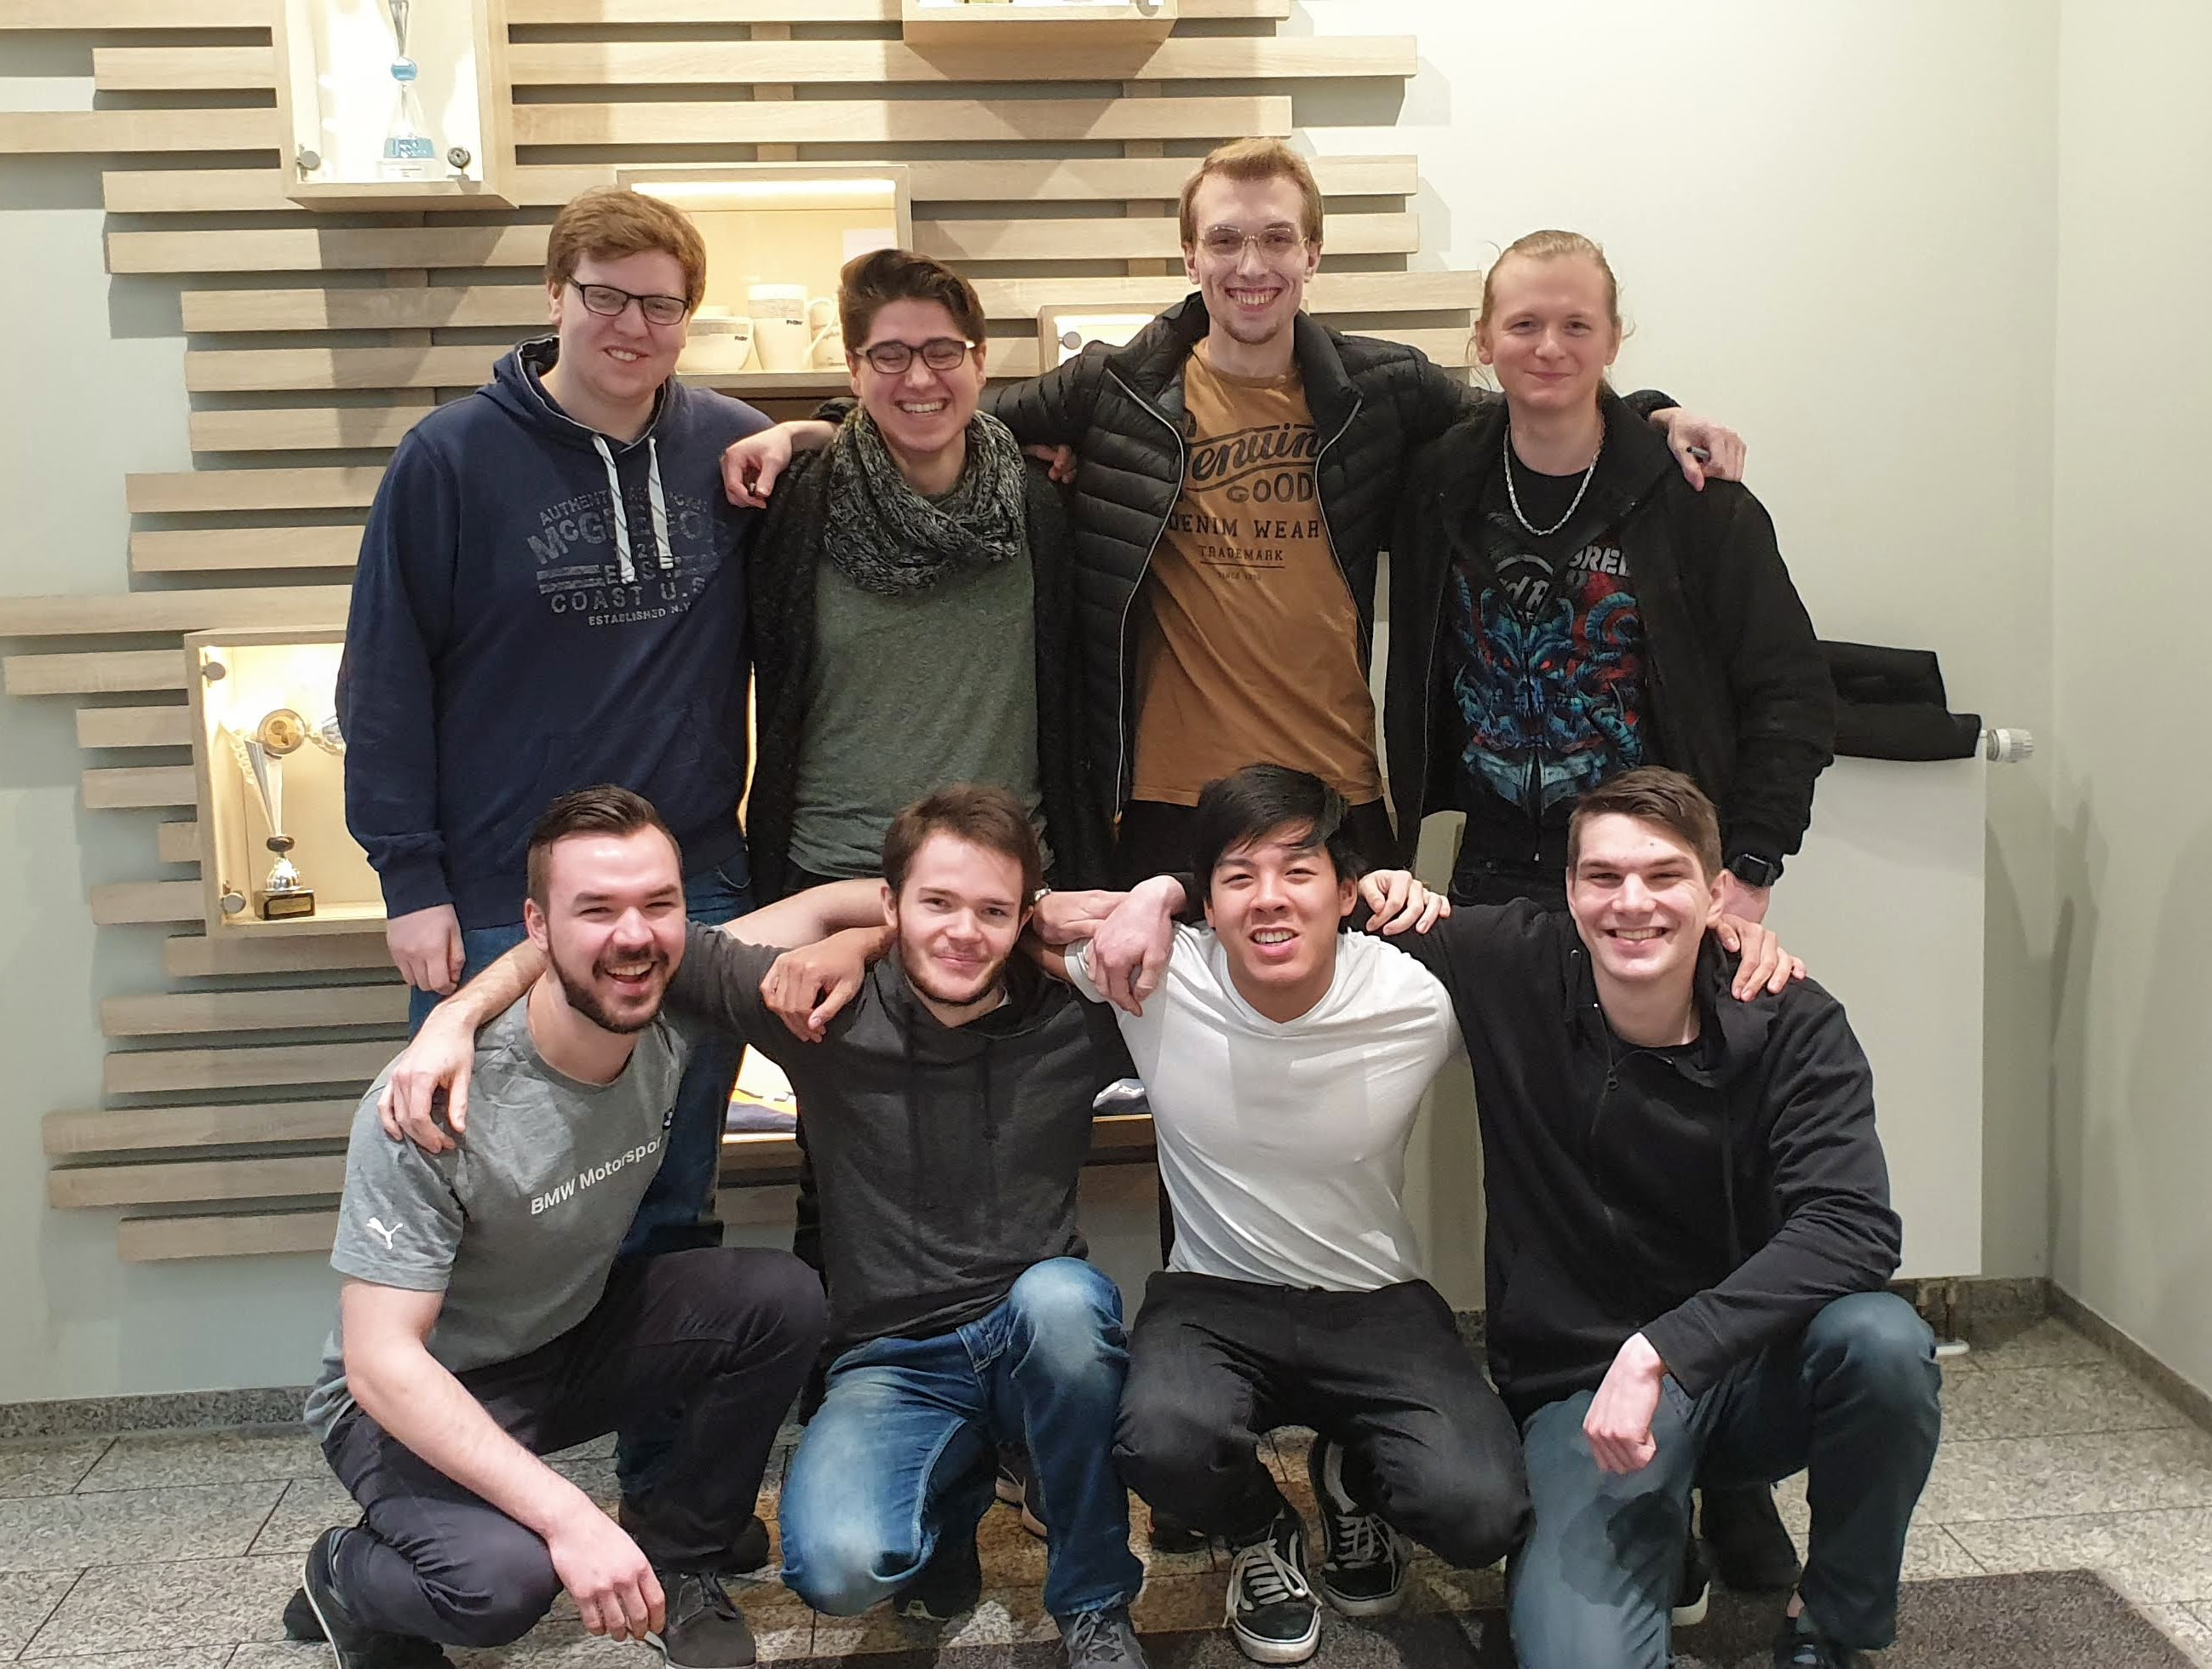
\includegraphics[width=\columnwidth]{img/teamfoto}
	\captionof{figure}{Gruppenfoto}\label{fig:gruppenfoto}
\end{figure}

\vfill

% Adjust this value if we replace images and they suddenly do not fit anymore.
\newcommand{\profilescale}{0.85}

\begin{table}[!htb]
	\centering
	\begin{tabularx}{\columnwidth}{XX}
		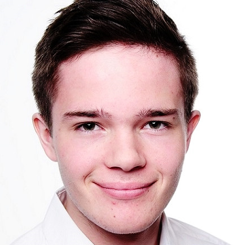
\includegraphics[scale=\profilescale]{img/profil-tom-bockhorn}
		\captionof{figure}{Tom Bockhorn}\label{fig:profil-tom-bockhorn}
			&	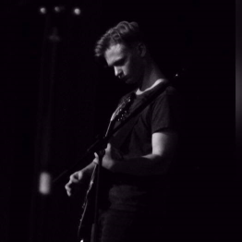
\includegraphics[scale=\profilescale]{img/profil-hendrik-falk}
				\captionof{figure}{Hendrik Falk}\label{fig:profil-hendrik-falk} \\
				
		
\includegraphics[scale=\profilescale]{img/profil-dennis-gentges}
		\captionof{figure}{Dennis Gentges}\label{fig:profil-dennis-gentges}
			&	
\includegraphics[scale=\profilescale]{img/profil-getuart-istogu}
				\captionof{figure}{Getuart Istogu}\label{fig:profil-getuart-istogu} \\
				
		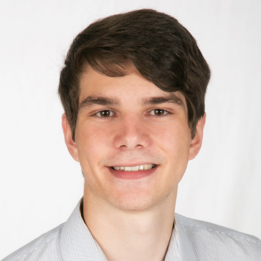
\includegraphics[scale=\profilescale]{img/profil-jannis-keienburg}
		\captionof{figure}{Jannis Keienburg}\label{fig:profil-jannis-keienburg}
			&	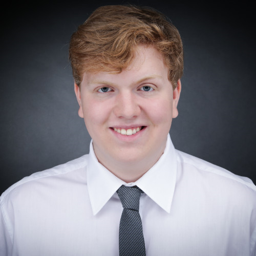
\includegraphics[scale=\profilescale]{img/profil-tim-meinerzhagen}
				\captionof{figure}{Tim Meinerzhagen}\label{fig:profil-tim-meinerzhagen}	\\
				
		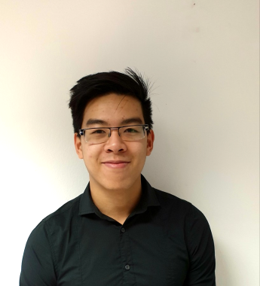
\includegraphics[scale=\profilescale]{img/profil-khang-pham}
		\captionof{figure}{Khang Pham}\label{fig:profil-khang-pham}
			&	
\includegraphics[scale=\profilescale]{img/profil-tim-schwenke}
				\captionof{figure}{Tim Schwenke}\label{fig:profil-tim-schwenke}
	\end{tabularx}
\end{table}



%!TEX root = ../Thesis.tex
\section{Ziel des Projektes [Falk]}

Das Ziel des Projektes ist die Entwicklung einer kachelbasierten Android-Applikation für den Auftraggeber Prof. Dr. Thomas Seifert. Diese Applikation soll die Funktion eines Taschenrechners nach der umgekehrten, polnischen Notation (UPN) erfüllen und wird im Folgenden als Tile Calculator bezeichnet. Dies stellt die Prüfungsleistung im Modul ''Projekte in der Wirtschaftsinformatik'' des Teams ''Das Proletariat'' dar. 

Das Team besteht aus folgenden Studierenden der Gruppe BFWI317B and der Fachhochschule der Wirtschaft Bergisch Gladbach: Tom Bockhorn, Hendrik Falk, Dennis Gentges, Getuart Istogu, Jannis Luca Keienburg, Tim Jonas Meinerzhagen, Khang Pham und Tim Schwenke. Diese absolvieren das Wirtschaftsinformatikstudium mit Schwerpunkt IT-Consulting als Angestellte und Auszubildende der Bayer AG, Bayer Business Services GmbH und der Currenta GmbH \& Co. OHG.

Der Projektzeitraum erstreckt sich vom 03.09.2019 bis zum 06.02.2020, wobei die Aufteilung der Zeit dem Team selber überlassen war.

Die zu entwickelnde Applikation, sowie der Prozess zur Erstellung selbiger soll ausführlich dokumentiert werden und zusammen mit der Applikation, welche auf der zur Verfügung gestellten Hardware installiert sein muss, eingereicht werden. 

Die folgenden Termine müssen eingehalten werden, damit das Projekt als erfolgreich gilt: 

\begin{itemize}
	\item \textit{05.09.2019:} Hochladen der aktuellen Version des Projekttagebuchs und Vorlage beim Dozenten.
	\item \textit{05.11.2019:} Hochladen der aktuellen Version des Projekttagebuchs.
	\item \textit{08.01.2020:} Hochladen der aktuellen Version des Projekttagebuchs.
	\item \textit{05.02.2020:} Hochladen der aktuellen Version des Projekttagebuchs.
	\item \textit{06.02.2020:} Hochladen der Individualversion der Studienarbeit und des Projektes (Deadline: 17:00).
	\item \textit{08.02.2020:} Präsentation des Projektergebnisses und Abgabe der ausgedruckten Team-Version der Studienarbeit sowie des zur Verfügung gestellten Tablets.
\end{itemize}

Alle hochzuladenden Dateien werden im vom Auftraggeber erstellten Microsoft Teams abgegeben.

%!TEX root = ../Thesis.tex
\section{Projektplanung}

\subsection{Beschreibung des Funktionsumfangs}

\subsection{Projektablaufplan}

\subsection{Planung der Software}

\subsubsection{Planung des Mockups}

\subsubsection{Planung der Datenstrukturen und Schnittstellen}

\para{Nutzung von Stack für Notation [Schwenke]}

Der Taschenrechner soll als Eingabelogik für die Anwendung von Operationen die umgekehrte polnische Notation verwenden. Hierbei werden immer zunächst die Operanden und im Anschluss daran die darauf auszuführenden Operatoren angegeben. Dieser Ansatz ermöglicht eine stapelbasierte Abarbeitung. 

Stacks werden, wie von den meisten Programmiersprachen, auch in Java in der Standardbibliothek unterstützt. Mit dabei sind Methoden wie \code{push} (für das Ablegen eines Objekts auf dem Stapel), \code{pop} (für das Entfernen und die Wiedergabe eines Objekts auf dem Stapel), \code{peek} (für die Wiedergabe ohne Entfernen eines Objekts auf dem Stapel) und \code{empty} (für das Leeren des Stapels). 

Jedoch müssen hierbei die besonderen Anforderungen des Taschenrechners beachtet werden. Operanden können von gänzlich unterschiedlichem Typus sein, zum Beispiel eine einfache Dezimalzahl oder auch ein Tupel, und viele Operationen benötigen mehr als die ersten (maximal zwei) Operanden auf dem Stack. Möchte man Elemente vom Stapel entfernen, kann man \code{pop} mehrmals aufrufen. Aufwändiger hingegen wird es bei \code{peek}. Möchte man mehrere Elemente vom Stapel einsehen ohne diese zu entfernen, muss man bei der Arbeit mit dem vorhandenen Stack einen weiteren bereithalten, nur um zwischengespeicherte Elemente lagern zu können. Anders ist es nicht möglich \code{peek} auf mehrere Elemente gleichzeitig anzuwenden. Gerade das ist aber bei der App notwendig. Weitere Methoden, die bei der umgekehrten polnischen Notation oft benötigt werden, aber nicht implementiert sind, sind \code{reverse} (für die Vertauschung der ersten zwei Elemente auf dem Stack, was wichtig für nicht-kommutative Operationen ist), \code{rollUp} (das unterste Elemente wird an den ersten Platz geschoben, das erste Element an den zweiten Platz usw.) und \code{rollDown} (das unterste Elemente wird an den ersten Platz geschoben, das erste Element an den zweiten Platz usw.).

Aufgrund dessen soll für dieses Projekt ein eigener Stapel implementiert werden. Dieser soll die zuvor genannten Funktionen mit unterschiedlichen Parametertypen unterstützen. Dabei ist darauf zu achten, dass die Programmierung generisch erfolgt und das Stack nicht nur alle Typen von Operanden unterstützt, sondern auch für gänzlich andere Klassenbäume in der App verwendet werden kann.

\para{Ansatz der Kalkulationsorchestrierung [Schwenke]}

Die App soll den Umgang mit unterschiedlichen Operanden-Typen beherrschen. Die Addition zweier Matrizen funktioniert anders als die Addition von zwei einfachen Dezimalzahlen. Java verfügt nativ weder über die entsprechenden Operanden noch über die Methoden für die Kalkulation. Auch die ausgewählte Bibliothek ist nicht ohne weiteres in der Lage Operationen auf alle Kombinationen von Operanden im folgenden Format einheitlich anzuwenden:

\texttt{Operation.mit(matrixOperand, dezimalOperand, dezimalOperand)}

Einheitlichkeit ist notwendig, damit im Frontend der Applikation keine Logik vorhanden sein muss, die entscheidet wie genau (auf Basis der Operanden-Typen) eine Operation umgesetzt wird. Deswegen muss eine einfache Schnittstelle entwickelt werden, die für den Nutzer nur zwei Drehschrauben bereitstellt. Dies ist zunächst die Auswahl der gewünschten Operation. Das kann z.B. das Symbol \code{+} als übliches Zeichen für Addition sein. Anschließend wird eine Reihe von Operanden übergeben. Dieser Aufruf sollte schließlich das Ergebnis in Form eines Operanden zurückgeben. Im Fall der Addition einer Matrix mit einer rationalen Zahl wäre dies wiederrum eine Matrix. Die korrekte Kalkulation soll also dynamisch bestimmt werden. Wichtig zu klären ist hier auch das Verhalten im Falle eines Fehlschlags. Nicht alle Kombinationen von Operanden können unterstützt werden. Die Verwendung von \textit{Optionals} (ein \code{Optional} ist ein Objekt, das man sich als Datenbehälter vorstellen kann, der entweder einen Wert enthält oder leer – aber nicht \code{null} sein kann) bietet sich hier zwar an, wird jedoch von Java in der verwendeten Android API-Version nicht unterstützt. Deswegen ist hier geplant sogenannte \textit{checked Exceptions} zu verwenden. Diese müssen bei der Verwendung explizit aufgefangen und weiterverarbeitet werden. Die Abbildung einer Operanden-Kombination auf die entsprechende konkrete Kalkulationsmethode muss dementsprechend zur Laufzeit des Programms erfolgen. Ein solches Mapping ist in Java nur mithilfe des Reflection-Pakets möglich. Reflektion ermöglicht den Einblick in ein Objekt (neben der Nutzung des Punkt-Operators) in eine Klasse. Zum Beispiel kann man eine Methode anhand einer Kombination von Parametertypen finden und aufrufen. Es ist geplant diesen Ansatz für die Orchestrierung der Kalkulationen in der App zu verwenden. Auch ist es nicht notwendig nur eine vordefinierte Anzahl an Argumente anzunehmen. So kann es sinnvoll sein, dass eine Methode zur Erstellung eines Tupels eine beliebige Anzahl an Operanden annimmt. Auch das lässt sich mit Reflektion umsetzen.

Der große Vorteil dabei ist, dass nirgendwo explizit in einer Abfrage entschieden werden muss, welche Kombination von Operanden an welche Methode weitergeleitet werden soll. Die Zuordnung erfolgt rein über die Deklaration der Parametertypen in der Methode selbst. Das macht das Ändern und Erweitern der Rechenfunktionalitäten einfach. Es muss lediglich die entsprechende Klasse herausgesucht und eine Methode im korrekten Format hinzugefügt werden. 

Zu entscheiden ist ebenfalls, ob das Gros der Rechenmethoden innerhalb der jeweiligen Operanden-Klassen oder dedizierten Klassen für die Kalkulation angesiedelt sind. Die erste Option hat neben der stärkeren Objektorientierung den Vorteil, dass immer klar ist, dass eine Methode mit den übergebenen Argumenten auf dem jeweiligen Objekt ausgeführt wird. Andererseits erhöht dies die Komplexität der Operanden-Klassen deutlich. Unterstützt man wie geplant 5 bis 7 dedizierte Typen von Operanden und 10 Kalkulationsarten, muss jede Klasse potenziell dutzende Methoden für die Rechnung enthalten. Die andere, und bevorzugte Option, ist die Auslagerung der Kalkulationsmethoden in eigenständige Klassen. Dies reduziert zwar nicht die Anzahl benötigter Methoden, isoliert die Rechenlogik jedoch in Klassen. Innerhalb dieser Klassen wird prozedural programmiert.  Eine typische Charakteristik von Objekten und deren Methoden ist \textit{Mutability}. Eine Methode bekommt ein Objekt und kann dieses verändern. Dies kann Testen unter Umständen aufwändiger gestalten. Durch Isolierung der Rechnungen in eigenen Klassen kann hingegen sichergestellt werden, dass jede Methode \textit{immutable}, also unveränderlich, ist. Das macht das Schreiben von Tests einfach. In Java kann Immutability durch die Verwendung von Annotationen sichergestellt werden. 

\subsubsection{Planung der Activities und Layouts}

\subsubsection{Planung der Navigation zwischen den Activities}

\subsection{Geplante Aufgabenverteilung im Team (tabellarisch)}

%!TEX root = ../Thesis.tex
\section{Beschreibung des Projektverlaufs}

\subsection{Tatsächliche Aufgabenverteilung im Team (tabellarisch)}

\subsection{Teammeeting-Protokolle}

 \para{03.09.2019 :: 200 Minuten}

\begin{itemize}
	\item Auswahl des Projekttyps. Das Team hat sich für die Entwicklung einer Android  App entschieden.
	\item Erste Einarbeitung in die Thematik. Lesen des bereitgestellten Dokuments mit Aufgabenstellung, groben Anforderungen und weiteres.
	\item Konzepterarbeitung auf Papier. Vorstellung und Diskussion verschiedener Ansätze.
\end{itemize}

\para{04.09.2019 :: 110 Minuten}

\begin{itemize}
	\item Sich mit Herr Seifert auf einen Ansatz für den Taschenrechner einigen.
	\item Workflow für Git, Meeting-Protokolle, Studienarbeit und Projekttagebücher festlegen.
	\item Ausarbeitung des Konzepts für den Taschenrechner. Hier wurden dem Auftraggeber Herr Seifert mehrere Konzepte vorgestellt und gemeinsam mit ihm genaue Anforderungen erarbeitet.
\end{itemize}

\para{05.09.2019 :: 20 Minuten}

Besprechen der Tagesziele:

\begin{itemize}
	\item Fertigstellung des Konzeptes.
	\item Fortschritte beim Paper-Prototypen machen bzw. erstellt haben.
	\item Android-Umgebung soll bei allen Team-Mitgliedern komplett aufgesetzt und lauffähig sein.
\end{itemize}

\para{05.09.2019 :: 60 Minuten}

Besprechen aktueller Stand des Konzepts und Prototypen:

\begin{itemize}
	\item Es wurde ein Mid-Fidelity Prototyp erstellt. 
	\item Diskussion über Umsetzung und Workflow der App.
	\begin{itemize}
		\item Wie sollen die einzelnen Kacheln funktionieren?
		\item Wie sollen die Kacheln miteinander interagieren?
		\item Wie könnte die Architektur der App aussehen?
	\end{itemize}
\end{itemize}

\para{05.09.2019 :: 40 Minuten}

\begin{itemize}
	\item Aufbau des Scrumboards mit Backlog, Doing, Review und Done.
	\begin{itemize}
		\item Backlog: Architektur Basics, Konzept (Paper Prototype, Mid-Fidelity-PPT-Prototyp), Rechenmodule, Zeitmanagement, UI-Coding-Design.
		\item Doing: Paper Mid Fidelity
		\item Review:
		\item Done: Git Projekt aufsetzen
	\end{itemize}
	\item Übertragen in Teams Planner und dort weitere Ausarbeitung.
	\item Grobe Verteilung der Einträge im Backlog um Konzepte zu erarbeiten.
\end{itemize}

\para{17.09.2019 :: 150 Minuten}

Backend-Architektur und App-Workflow:

\begin{itemize}
	\item Erweiterung UML-Klassendiagramm. Die Klasse Operand wird abstrakt und wird von konkreten Operanden wie Vector geerbt. Diese stellen Extensions dar die neben den eigentlichen mathematischen Werten weitere Daten und Verhalten mitbringen.
	\item Welche Library soll für Mathe-Funktionalitäten benutzt werden? JScience und die bereits mitgelieferte Standardbibliothek.
	\item Wie sollen Elemente in der GUI dargestellt werden? Als ASCII oder gerendert in LaTeX. Letzteres ist mit höherer Komplexität verbunden sieht aber auch besser aus. 
	\item Wie soll das Layout funktionieren? Gridlayout fällt raus, weil nicht dynamisch genug? Relative-Layout ist eine Option. Hier darf aber die Anordnung beim Rotieren nicht unkontrolliert verändert werden. UI Team möchte, dass alle Komponenten gleich groß sind. In dem Fall kann man Gridlayout benutzen.
	\item Wie soll die Eingabe von Funktionen im Graph Operand funktionieren? Nur möglich mit bereits vorhandenen Elementen in der Oberfläche. Es öffnet sich keine Tastatur.
\end{itemize}

\para{09.10.2019 :: 90 Minuten}

Verteilung von Programmieraufgaben und Diskussion:

\begin{itemize}
	\item Vorstellung des Backend-Entwurfs für Teammitglieder, die für das Frontend zuständig sind. 
	\item Vorstellung des Frontend-Entwurfs für Teammitglieder, die für das Backend zuständig sind.
	\item Diskussion über Verbindung von Frontend und Backend. Wie abgekoppelt lässt sich der Calculator wirklich realisieren?
	\item Vorstellung der Hauptbibliothek die für die (aufwändigen) Rechnungen wie Nullstellenberechnung benutzt werden soll.
	\item Warum Apache Commons Math und nicht JScience?
	\item Diskussion des Programm-Workflows.
	\item Diskussion ob ASCII-Darstellung oder LaTeX-Rendering für Frontend benutzt werden soll
\end{itemize}

\para{05.01.2020 :: 120 Minuten}

Arbeit am Projekt:

\begin{itemize}
	\item Aufnahme des aktuellen Projektstands.
	\item Besprechen des weiteren Vorgehens.
	\item Aufgabenabstimmung.
	\item Besprechung des geplanten Frontends.
	\item Besprechung/ Lösung von Problemen.
\end{itemize}

\para{14.01.2019 :: 90 Minuten}

Zusammenführung Frontend Backend:

\begin{itemize}
	\item Präsentation des Frontends durch das GUI-Team.
	\item Besprechen von MVC-Umsetzung in Android.
	\item Backend Unit-Testing Fortschritte.
	\item Serialisierung der Stacks zur Session-Sicherung.
\end{itemize}

\para{24.01.2019 :: 240 Minuten}

\begin{itemize}
	\item Detaillierte Ausarbeitung der Architektur im Backend.
	\item Programmieren im Team. 
	\item Zusammenführen mehrere Features.
	\item Umbau der Programmstruktur.
\end{itemize}

\para{28.01.2019 :: 90 Minuten}

Gespräch mit Herr Prof. Dr. Thomas Seifert über den aktuellen Stand des Projekts und im Anschluss daran eine Nachbesprechung innerhalb des Teams.

Vorstellung:

\begin{itemize}
	\item Vorstellung der bereits implementierten Grundfunktionen der App.
	\item Vorstellung des verwendeten Design-Patterns.
	\item Abgleich von Umsetzung mit den Anforderungen des Dozenten.
	\item Ansatz des Backends erklärt.
	\item Gerät ausleihen, um nicht nur mit Emulator testen zu können.
	\item Serialisierung der Daten (Speichern und Laden).
\end{itemize}

Ergebnis:

\begin{itemize}
	\item Projekt ist auf einem guten Weg. Priorisiert werden sollen differenzierende Funktionen anstatt wenige Features sehr detailliert auszuarbeiten (Prototypische Arbeit).
	\item Ternäre, Quaternäre usw. Operationen sind gewünscht.
	\item Vektoren in Bestandteile lösen.
	\item Eingabe von Matrizen.
	\item Jeder Klasse muss ein Verantwortlicher zugeordnet sein.
\end{itemize}

Ideen aus der Nachbesprechung:

\begin{itemize}
	\item ''Vektor bauen'' / ''Vektoren auflösen'' Action. 
	\item Summe von Stack Action.
	\item 1x Triple Operator einfügen.
	\item Operanden Eingabe via einzelne Menüs.
	\item Ranks der Stacks anpassen.
	\item Format des ersten Stacks anpassen (Format nicht 0,00).
\end{itemize}

\subsection{Projekttagebücher aller Teammitglieder (tabellarisch)}

\subsubsection{Tom Bockhorn}

\subsubsection{Hendrik Falk}

\subsubsection{Dennis Gentges}

\subsubsection{Getuart Istogu}

\subsubsection{Jannis Keienburg}

\subsubsection{Tim Jonas Meinerzhagen}

\subsubsection{Khang Pham}

\subsubsection{Tim Schwenke}

\subsection{Beschreibung von Problemen}

\subsubsection{Softwareentwicklung im Team [Schwenke]}

Schon kurz nach der initialen Erstellung des Git-Repositories und des Projekts in Android-Studio hat sich die Frage gestellt, wie man in einem acht Mitglieder starkem Team produktiv an einer einzelnen Code-Basis arbeiten soll. Hat man ein Quellcodeverzeichnis alleine für sich reichen zumeist um die drei aktive (also nicht \textit{stale}) Branches aus. Das wäre zunächst der \code{Master}-Branche, welcher die Wurzel des Verzeichnisses darstellt und – gerade, wenn Ansätze wie CI/CD verfolgt werden – die produktiven oder zumindest lauffähigen Versionen eines Projekts enthält. Im \code{Development}-Branch hingegen findet die Entwicklung statt. Hier ist es üblich, dass das Projekt zum Zeitpunkt einzelner Commits Fehler enthält und nicht lauffähig ist. Sobald ein Entwickler der Meinung ist, dass der Stand in \code{Development} veröffentlicht werden kann, wird \code{Development} in \code{Master} vereint. Wichtig zu betonen ist hier, dass dies keine feste Regel ist, sondern eher dem allgemeinen Workflow entspricht. In einem großen Team ist ein solcher Arbeitsablauf nicht mehr möglich. So müssen mehrere Entwickler parallel an dem Projekt arbeiten. Verwendet man nun das System aus zwei Branches, wird es sehr schnell zu Merge-Konflikten kommen, die die Entwickle dazu zwingen sich mehr mit der korrekten Zusammenführung als der eigentlichen Entwicklung zu beschäftigen, sofern sie ihren lokalen Arbeitsbereich aktuell halten wollen. Die nächstliegende und ebenfalls problematische Alternative ist es nur bei Fertigstellung von Funktionen, die meist aus mehreren Commits zusammengesetzt sind, das lokale Quellcodeverzeichnis mit dem Remote zu synchronisieren. Mit dieser Herangehensweise verpasst man unter Umständen große Fortschritte im Gesamtprojekt. Die lokale Version ist plötzlich nicht mehr lauffähig und muss aufwändig angepasst werden. Deswegen haben wir uns in diesem Projekt für den Gitflow-Workflow entschieden. Grafisch dargestellt ist dieser beispielhaft in der folgenden Grafik.

\begin{figure}[h]
	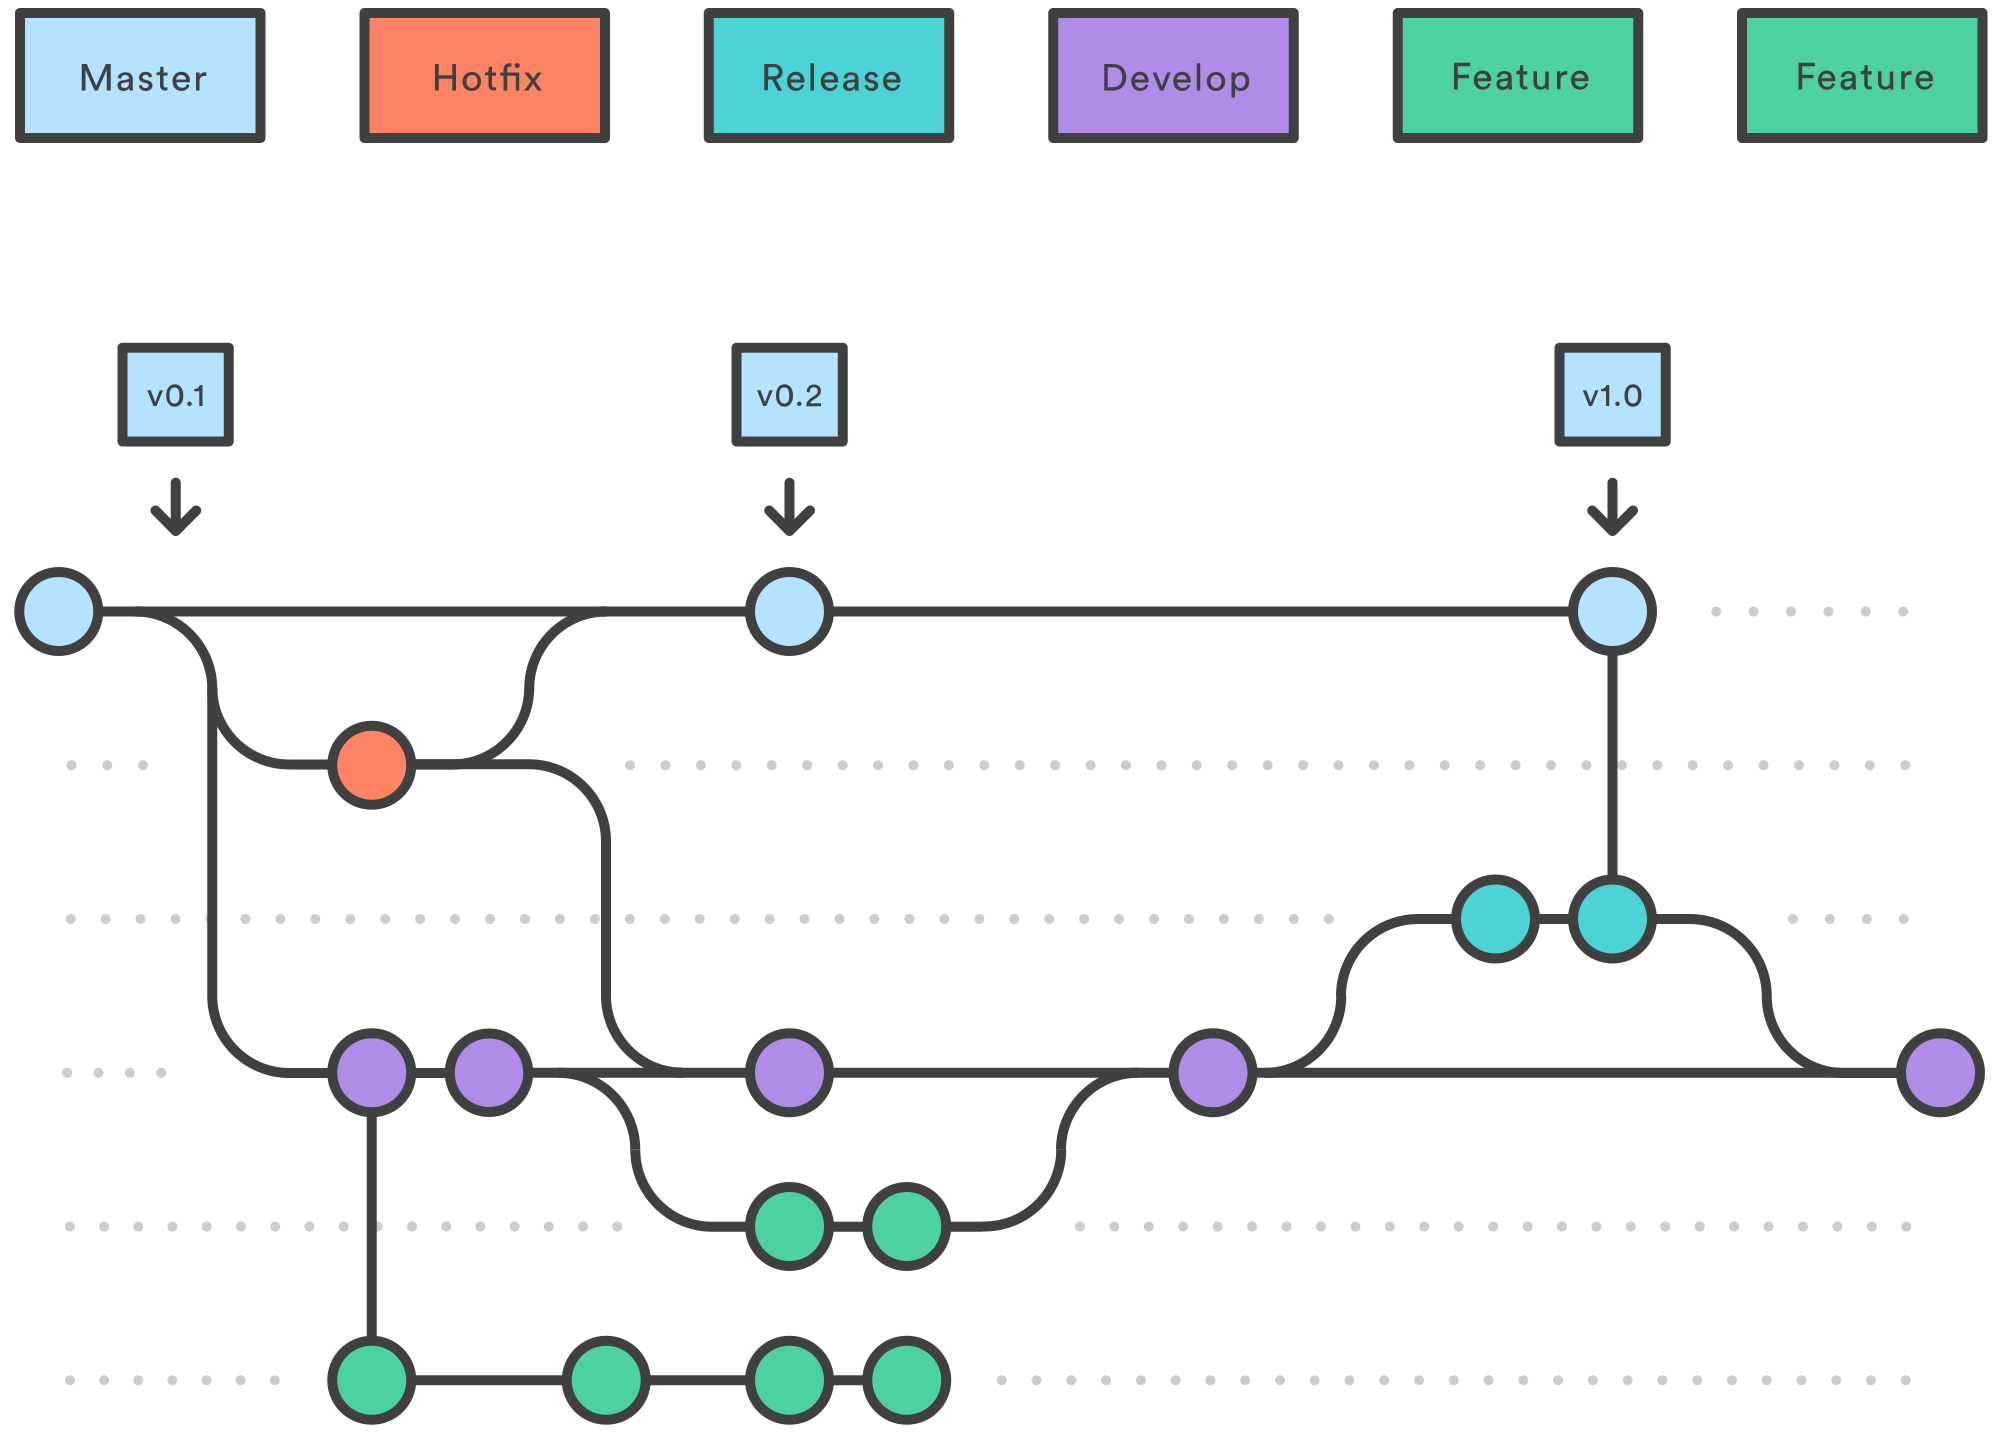
\includegraphics[width=\columnwidth]{img/gitflow}
	\caption[Gitflow]{Gitflow\footnotemark}
\end{figure}
\footnotetext{\cite{atlassian2020}}

Der Gitflow-Workflow definiert ein strenges Branching-Model und gibt jedem Typ von Branch (lediglich differenziert durch ihre Namen) eine spezifische Rolle. \code{Master} wird verwendet, um die Release-History festzuhalten. Hier finden sich Versionen des Projekts, die lauffähig sind und für sich alleine stehen (können). \code{Development} fungiert ähnlich wie \code{Master}, nur enthält es die gesamte Entwicklungshistorie des Projekts. Nun kommen die sogenannten \code{Feature}-Branches ins Spiel, die beliebig weiter untergliedert werden können. Benannt werden Features hierarchisch. In unserem Projekt haben wir folgende zwei Gruppen von Feature-Branches: 

\texttt{feature/backend/<konkretes-feature>}

\texttt{feature/frontend/<konkretes-feature>}

Jedes Feature wird einem Verantwortlichen zugeteilt und wird meist auch von diesem bearbeitet. Sobald ein Feature fertig ist, wird es in \code{Development} zusammengeführt. Somit werden die Abstände zwischen Zusammenführungen verringert und der Arbeitsablauf wird einfacher. Schließlich gibt es auch noch einen Hotfix-Branch, für dringende Änderungen.

Im Laufe der Entwicklung haben sich die Vorteile dieser Herangehensweise für das Team deutlich gezeigt. Unterschiedliche Features konnten, nachdem eine grundlegende Programmarchitektur umgesetzt wurde, meist ohne Probleme zusammengeführt werden. 

%!TEX root = ../Thesis.tex
\section{Dokumentation der Software}

\subsection{Dokumentation der Paketstruktur des Android-Projektes [Falk]}

Die Applikation liegt im Paket \code{de.fhdw.wip.rpntilecalculator} und ist in einzelne Klassen unterteilt, welche in eine Ordnerstruktur eingebettet sind. Diese Ordnerstruktur orientiert sich an dem gewählten UI Design Pattern MVP. Dabei gibt es einen Model Ordner. Dieser ist in vier weitere Ordner unterteilt, welche den Kachelarten nachempfunden sind und einen für den Stack. In diesen befinden sich verschiedene Klassen, die zusammen das Model bilden. Im \code{Presenter}-Ordner befindet sich lediglich der Presenter. Der \code{View}-Ordner besteht wieder aus mehreren Teilen. Zum einen aus der \code{MainActivity}, welches die Hauptansicht der Appliaktion darstellt. Dazu befinden sich dort Typen und Grundklassen der Kacheln. Es gibt noch die drei Ordner \code{Layout}, \code{Menu} und \code{Schemes}. In \code{Layout} befinden sich Funktionen zum Darstellen, Speichern und Laden der Kacheln. In \code{Schemes} befinden sich Vorlagen für Tiles und in \code{Menu} sind sämtliche Menüs gespeichert. 

\begin{figure}[!h]
	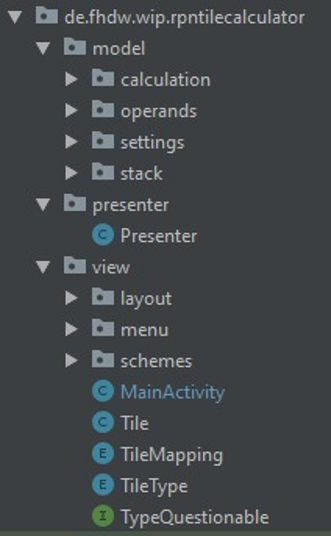
\includegraphics[scale=1]{img/ordnerstruktur}
	\caption[Ordnerstruktur]{Ordnerstruktur\footnotemark}
\end{figure}
\footnotetext{eigene Darstellung (Screenshot aus Android Studio)}

\begin{figure}[!h]
	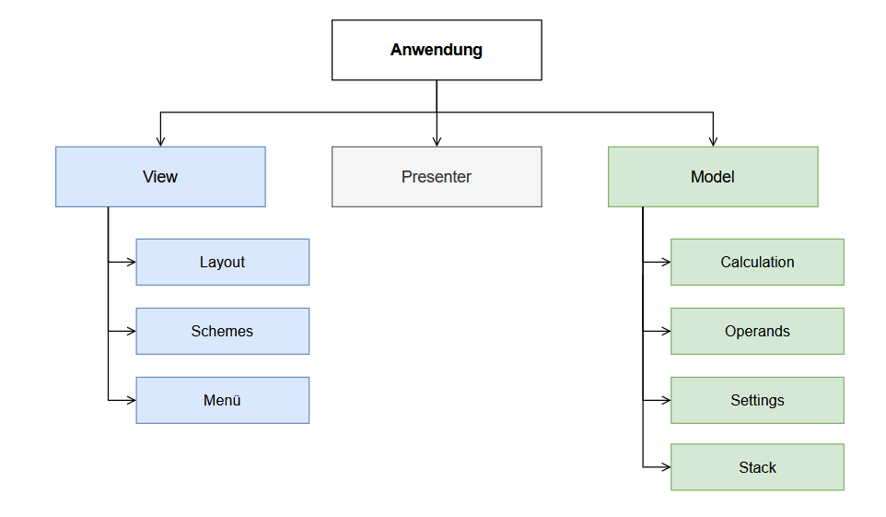
\includegraphics[scale=1]{img/ordnerstruktur2}
	\caption[Ordnerstruktur Schema]{Ordnerstruktur Schema\footnotemark}
\end{figure}
\footnotetext{eigene Darstellung}

\subsection{Dokumentation der View}

In den folgenden Kapiteln wird die Implementierung des Frontends der Applikation, der sogenannten View, und jeglichen zugehörigen Implementierungen, dargestellt.

\subsubsection{Activities [Bockhorn]}

Die Applikation wird durch den Aufruf der sogenannten \code{MainActivity} vom Android System beim Öffnen der Anwendung gestartet. Da die Menüführung nicht auf Activities basiert und jegliche Layouts dynamisch geladen werden, bleibt die \code{MainActivity} die einzige Activity der Applikation

Im MVP Pattern ist die \code{Activity} der View zugeordnet. Sie lädt unter anderem vertikale und horizontale Layouts vor und stellt eine Methode zur Darstellung dieser bereit. Auch wird ein Listener erstellt, der nach Änderungen der Bildschirmausrichtung horcht und passende Layouts lädt.

\paragraph{Klasse: MainActivity}

\textbf{Beschreibung:} Activity, die beim Starten der Anwendung aufgerufen wird und das Layout \code{activity\_main.xml} aufruft. Dieses Layout ist jedoch leer, da alle Inhalte dynamisch geladen werden. Es lädt auch Taschenrechner-Layouts vor und stellt Methoden zur Darstellung dieser bereit.

\textbf{Methode} \code{onCreate()} lädt die Layouts vor, erstellt einen \code{Listener} ob die Orientierung sich verändert und öffnet das erste Layout.

\textbf{Methode} \code{setTileLayout()} lädt ein Layout in die View.

\subsubsection{Generische Kachelgestaltung [Bockhorn]}

Die generische Gestaltung der Kacheln wurde gemäß dem Entwurf so umgesetzt, dass eine Trennung zwischen Kacheln, die als Buttons vom Kontext der Applikation abhängig sind, und Kacheln, die vom Kontext unabhängig sind, ermöglicht wird. Dies dient unter anderem dem Vorladen von Layouts zur Optimierung der Ladeperformance. Außerdem wird so die Definition des Kacheltypen und dessen spezialisierte Inhalte auf die vom Kontext unabhängigen Kachelschemata (\code{TileSchemes}) ausgelagert. 

Als logische Abtrennung kann man sich merken, dass Kacheln (\code{Tiles}) lediglich für die Kommunikation mit dem Nutzer zuständig sind, während die \code{TileSchemes} die restliche Frontend-Logik beinhalten.

\subsubsection{Kontextbezogene Kacheln [Bockhorn]}

Die Tiles werden mit Bezug auf den Kontext, also die aktuell dargestellte Activity, erstellt. Sie dienen als generische Kachelklasse, dessen Funktionalitäten unabhängig vom Kacheltypen gebraucht werden.

Ein Tile, als Unterklasse des \code{AppCompatButton} von Android, wirft beim Anklicken ein Event, welches von registrierten \code{OnClickListenern} abgefangen werden kann. Für die einzelnen Tiles wird der \code{Presenter} als \code{OnClickListener} registriert, sodass dieser die vom Nutzer getätigten Klicke verarbeiten kann. Zusätzlich wird dem \code{Tile} als \code{OnLongClickListener} das Menü \code{TileTypeInput} übergeben, welches bei langem Klicken geöffnet wird und somit die Bearbeitung des Kacheltypen ermöglicht.

\begin{figure}[!h]
	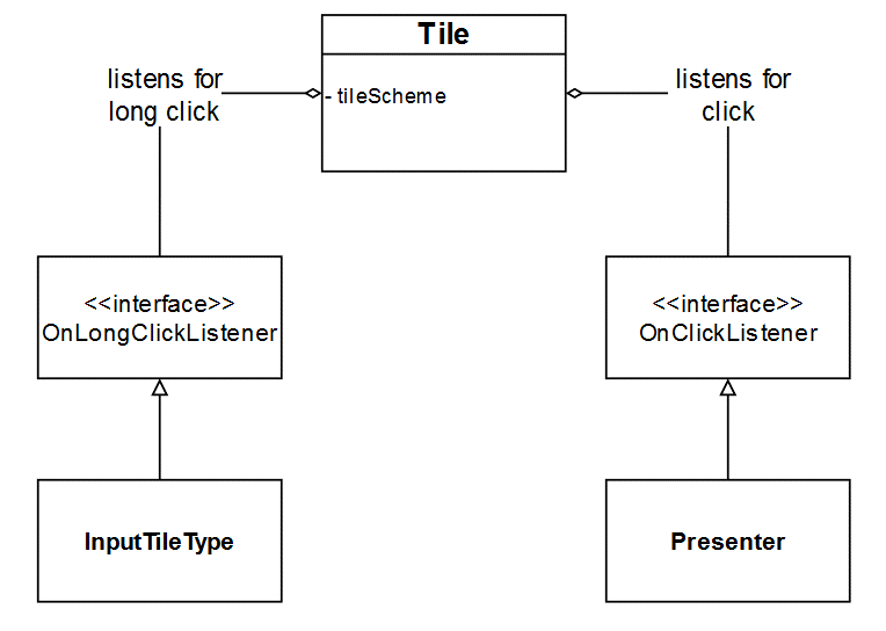
\includegraphics[scale=1]{img/listener-von-tile}
	\caption[Listener von Tile]{Listener von Tile\footnotemark}
\end{figure}
\footnotetext{eigene Darstellung}

Die Informationen über den Kacheltypen des \code{Tiles} befindet sich im \code{TileScheme} des \code{Tiles}. Werden nun die Inhalte, oder gar der Kacheltyp des \code{Tiles} verändert, so wird das Aussehen des \code{Tiles} anhand des aktuellen \code{TileSchemes} aktualisiert. Ähnlich stellt ein \code{Tile} verschiedene Animationen bereit, die zum Beispiel beim Laden oder Speichern des \code{Tiles} aufgerufen und abgespielt werden können.

\paragraph{Tile [Bockhorn]}

\textbf{Superklasse:} \code{AppCompatButton}

\textbf{Beschreibung:} Agiert als Button auf einem Kontext, dessen Inhalt und Typ durch ein \code{TileScheme} definiert sind. Einfaches Klicken wird vom \code{Presenter} abgefangen und gedrückt halten öffnet ein Auswahlmenü für die Kachelart. 

\textbf{Methode} \code{update} Aktualisiert das \code{Tile} mithilfe eines neuen \code{Schemes}. Setzt dabei Hintergrund Ressource und Text

\textbf{Methode} \code{enableMenulistener} Aktiviert die Menüfunktion für dieses \code{Tile}

\subsubsection{Kontextfremde Kacheln [Gentges]}

Die \code{TileSchemes} stehen in keiner Beziehung zum Kontext der Anwendung. Dennoch wird in ihnen der Text und das Design des letztendlichen \code{Tiles} gespeichert. Im Gegensatz zu den \code{Tiles} differenzieren \code{TileSchemes} hier zwischen Kachelarten. Die Grundeigenschaften eines \code{TileSchemes}, also die Information darüber um welche Art von Kachel es sich handelt, und was genau der Inhalt ist, werden in der Superklasse \code{TileScheme} definiert. Ersteres liegt in Form eines sogenannten \code{TileMappings} vor. Für jede der bestehenden Kachelarten wurde eine Unterklasse implementiert, welche die Eigenschaften von \code{TileScheme} erbt und weitere artbezogene Inhalte definiert. In Kombination mit einem \code{Tile} können so andere Komponenten der Applikation, wie beispielsweise der \code{Presenter}, die Kachelart des \code{TileScheme} erfragen und den vorliegenden Inhalt für die auszuführenden Prozesse extrahieren.

\begin{itemize}
	\item Das \code{ActionTileScheme} ist die Implementierung eines \code{TileScheme} vom Typ Action, (auch \code{Operator}) der Inhalt und Typ um eine instanziierte Action erweitert. Dank der ähnlich polymorphen Struktur der \code{Action}s, kann so mit einem simplen Methodenaufruf jede Form von \code{Action}, die im Schema hinterlegt ist, angesprochen und ausgeführt werden.
	\item Ein \code{SettingTileScheme} erbt ebenfalls von \code{TileScheme}, aber liefert zusätzlich Informationen über ein sogenanntes \code{Setting}, welches ähnlich wie eine \code{Action} über eine vererbte Methode anzusprechen ist.
	\item Ein \code{OperandTileScheme} ist gleich aufgebaut, beinhaltet aber Operanden, die als Grundlage für die Kalkulation mit \code{Action}s dienen.
	\item Das Klicken auf ein \code{Tile} des Stacks wird intern gleich gehandhabt, wie das Klicken eines Operanden. Jedoch besitzen Tiles aus dem Stack eine Reihenfolge, die im \code{StackTileScheme} als Rang hinterlegt wird. Um die gleiche Behandlung eines potenziellen Operanden im Stack zu gewährleisten, erbt \code{StackTileScheme} nicht von \code{TileScheme}, sondern von \code{OperandTileScheme}. 
	\item Ein \code{HistoryStackTile} ist ebenfalls so aufgebaut, wie ein \code{StackTileScheme}, und erbt daher dessen \code{Attribute}.
\end{itemize}

Die Erstellung einzelner \code{TileSchemes} erfolgt mithilfe des Factory-Method-Design-Pattern. Hierzu stellt die abtrakte Superklasse \code{TileScheme} zwei Methoden zur Verfügung. Innerhalb dieser Methoden wird anhand des \code{TileMappings} zwischen den verschiedenen Kachelarten differenziert und der passende Konstruktor der Unterklasse aufgerufen. In einer Methode erfolgt die Erstellung des \code{TileScheme} Inhalts durch die Einlese eines Zeichenkette. Dies findet beispielsweise bei der Kreierung von \code{TileSchemes}, nach der Auslese eines im internen Speicher gespeicherten Layouts, Anwendung. Als zweite Option kann aus einem bereits bestehenden Operanden ein \code{TileScheme} der Art Operand, Stack oder Historie erstellt werden. Dadurch, dass Stack und Historie eines Layouts regelmäßig aktualisiert werden müssen, bietet sich die performante Erstellung von \code{TileSchemes} mithilfe bestehender Operanden, gegenüber der aufwendigen erneuten Auslese aus einem String, an.

Im Kontrast zu den Tiles, die eine Methode zum Aktualisieren der Inhalte bereitstellen, müssen \code{TileSchemes} mithilfe der genannten Methoden rekreiert werden. Kann eine Kachelart nicht identifiziert werden, oder sind die Angaben über den Inhalt der Kachel unkorrekt, so wird ein \code{ErrorTileScheme} erstellt, das visuell von jeder anderen Art zu unterscheiden ist und den Entwicklern somit über den Fehler Bescheid gibt.

\paragraph{Abstrakte Klasse: TileScheme}

\textbf{Beschreibung: }Abstrakte Superklasse, die neben den artübergreifenden Inhalten der \code{TileSchemes}, Methoden zur Kreierung dieser gemäß des Factory-Method-Design-Pattern bereitstellt.

\textbf{Methode} \code{createTileScheme()} liefert in Abhängigkeit vom angegebenen \code{TileMapping} eine Instanz einer Unterklasse des \code{TileSchemes}. Die Erstellung von \code{TileSchemes} für \code{Actions} und \code{Settings} ist lediglich durch die Eingabe von Zeichenketten möglich. \code{TileSchemes} der Arten \code{Operanden}, \code{Stack} und \code{Historie} können zusätzlich aus bestehenden \code{Operanden} erstellt werden. 

\paragraph{Klasse: ActionTileScheme}

\textbf{Superklasse:} \code{TileScheme}

\textbf{Beschreibung:}\code{TileScheme} für Operatoren. \code{Action}, die ausgeführt werden soll, als Zusatzinformation. Inhalt ist der Text der Kachel.

\paragraph{Klasse: SettingTileScheme}

\textbf{Superklasse:} \code{TileScheme}

\textbf{Beschreibung:} \code{TileScheme} für Einstellungen. \code{Settings}, die ausgeführt werden soll, als Zusatzinformation. Inhalt ist der Text der Kachel. 

\paragraph{Klasse: OperandTileScheme}

\textbf{Superklasse:} \code{TileScheme}

\code{Beschreibung:} \code{TileScheme} für Operanden. Bei der Erstellung aus Text wird der String mithilfe \textit{Reflections} zu einem Operanden übersetzt.

\paragraph{Klasse: StackTileScheme}

\textbf{Superklasse:}\code{OperandTileScheme}

\textbf{Beschreibung:}\code{TileScheme} für Operanden im Stack. Wird genauso behandelt wie ein \code{OperandTileScheme}, doch verfügt zusätzlich über eine Information über den Rang der Kachel im gesamten Stack.

\paragraph{Klasse: StackTileScheme}

\textbf{Superklasse:} \code{OperandTileScheme}

\textbf{Beschreibung:} \code{TileScheme} für Operanden im Stack. Wird genauso behandelt wie ein \code{OperandTileScheme}, doch verfügt zusätzlich über eine Information über den Rang der Kachel im gesamten Stack.

\paragraph{Klasse: HistoryTileScheme}

\textbf{Superklasse:} \code{StackTileScheme}

\textbf{Beschreibung: }\code{TileScheme} für Operanden in der Historie. Wird genauso behandelt wie ein \code{OperandTileScheme}, doch verfügt zusätzlich über eine Information über den Rang der Kachel im Gesamtstack.

\paragraph{Klasse: ErrorTileScheme}

\textbf{Superklasse:} \code{TileScheme}

\textbf{Beschreibung: }\code{TileScheme} für die Ausnahmesituation, dass ein reguläres \code{TileScheme} nicht geladen werden konnte

\subsubsection{Kacheltypdefinition durch Enumartion [Pham]}

Wie zuvor erläutert, erstellt die Klasse \code{TileSchemes} ein passendes Schema anhand eines sogenannten \code{TileMappings}. Ein \code{TileMapping} ist im Endeffekt eine konkrete Definition einer Kachel im Frontend-System. Hierzu beinhaltet das entsprechende \code{TileMapping} jegliche Informationen, die für eine bestimmte Kachel von Relevanz ist. 

Durch die Deklaration als Enum werden diese Informationen mit einer Zeichenkette zur Einlese in Verbindung gebracht. 

Für den Operator \code{-} (\code{Minus}) ist dies beispielsweise die Kachelart (\code{Action} / \code{Operator}), eine Referenz auf die passende \code{Action} Klasse und den Anzeigetext der Kachel \code{-}, die mit dem Text \code{A\_MINUS} betitelt werden. 

Die einzelnen Definitionen liegen in Form einer Java-Enumeration vor, da diese Ein Beispiel für eine solche Definition sieht wie folgt aus:

\code{A\_MINUS(TileType.ACTION, Minus.getInstance(), "-")}

Neben Operatoren werden im Enum die anderen Datentypen ebenfalls angelegt. Technisch wurde dies durch die Verwendung von überladenen Konstruktoren ermöglicht und die \code{TileSchemes} wissen welche Informationen gebraucht werden. Zur Definition der Kachelart selbst wurde eine weitere Enumeration mit folgenden Werten angelegt:

\begin{itemize}
	\item \code{Stack}
	\item \code{History}
	\item \code{Operand}
	\item \code{Action}
	\item \code{Setting}
	\item \code{Error}
\end{itemize}

Zu den Kachelarten sind Design-Ressourcen hinterlegt, welche die Gestaltung der Kacheln je nach Typ definiert.

\paragraph{Enumeration: TileMapping}

\textbf{Beschreibung: }Definiert Kacheln und dessen wichtigste Elemente. Wird außerdem zur Einlese von Texten genutzt.

\textbf{Bsp:} \code{A\_MINUS(TileType.Action, Minus.getInstance(), '' -'')}

\paragraph{Enumeration: TileType}

\textbf{Beschreibung: }Definiert die verschiedenen Kachelarten und ihre Design Ressourcen

\textbf{Bsp:} \code{ACTION(R.drawable.tile \_operator \_blue)}

\subsubsection{Gruppierung der Kacheln im Layout Container [Bockhorn]}
Gemäß dem Entwurf werden die Kacheln, sowohl \code{Tiles} als auch \code{TileSchemes}, in einem einheitlichen Container gespeichert. Das sogenannte \code{TileLayout} beinhaltet und bietet so dem Presenter eine zentralisierte Stelle zur Kommunikation mit Kacheln.

Insgesamt werden drei Bereiche unterstützt:
\begin{enumerate}
	\item Das Laden von kontextfremden \code{TileSchemes} in kontextbezogene \code{Tiles}. Grundsätzlich ist das \code{TileLayout} zwar unabhängig vom Applikationskontext, kann jedoch per Methode eine View für einen Kontext erstellen. Die Übersetzung erfolgt mit einer Darstellung in einer sogenannten \code{TableView} von Android. Neben der zweidimensionalen Liste an \code{Tiles} werden Listen für Stack und Historie geführt, die dann getrennt adressierbar sind.
	\item Die Aktualisierung von \code{Tiles} bei Änderungen im Stack, der Historie oder Anpassungen des Layouts. Hierbei ist zu erwähnen, dass nie das gesamte Layout aktualisiert wird, sondern nur Stack oder Historie. Beide werden mithilfe der korrespondierenden Listen im Presenter verglichen und aufgefüllt. Die Aktualisierung eines \code{Tiles} erfolgt durch die Kreierung eines neuen \code{TileSchemes}.
	\item Das Speichern des aktuellen \code{TileLayouts} durch die Zurückübersetzung von kontextbezogenen \code{Tiles} in kontextfremde \code{TileSchemes} zur Weiterverarbeitung durch den sogenannten \code{TileLayoutLoader}.
\end{enumerate}
Das \code{TileLayout} selbst wird mithilfe der \code{TileLayoutFactory} unter Verwendung des Factory-Design-Patterns aus einer Zeichenkette geladen. Das persistente Speichern und Laden dieser Zeichenkette und der Bezeichnung des \code{TileLayouts} selbst wird vom \code{TileLayoutLoader} orchestriert (siehe Kapitel~\ref{subsection:dokumentation-der-persistenten-datenhaltung}).

\para{Klasse: TileLayout}
\textbf{Methode} \code{createView} erstellt eine zweidimensionale Liste an \code{Tiles} aus der zweidimensionalen Liste an \code{TileSchemes}. Währenddessen werden eine \code{TableView} zusammengebaut und zurückgegeben und den eigenen Stack und die Historie Listen gesetzt.

\textbf{Methode} \code{pushStack2Presenter} übergibt dem Presenter den aktuellen Stack, z.B. zum Laden der Anwendung

\textbf{Methode} \code{pushHistoryStack2Presenter} übergibt den aktuellen History Stack, z.B. zum Laden der Anwendung

\textbf{Methode} \code{updateStack} aktualisiert jegliche \code{Tiles} im Stack durch den im Presenter geführten Stack an Operanden

\textbf{Methode} \code{updateHistoryStack} aktualisiert jegliche \code{Tiles} im History Stack durch die im Presenter geführte Historie

\textbf{Methode} \code{generateLayoutText} Generiert eine Zeichenkette im CSV-Format anhand der zweidimensionalen Liste an \code{Tiles}

\para{TileLayoutFactory}
\textbf{Beschreibung}: Factory für \code{TileLayouts}, die anhand einer Zeichenkette ein passendes Layout erstellt

\textbf{Methode} \code{createView} erstellt eine zweidimensionale Liste an \code{Tiles} aus der zweidimensionalen Liste an \code{TileSchemes}. Währenddessen werden eine \code{TableView} zusammengebaut und zurückgegeben und den eigenen Stack und die Historie-Listen gesetzt.

\subsubsection{Implementierung der Menüsteuerung [Istogu]}

In diesem Abschnitt wird die Umsetzung der Planung für die Menüsteuerung aufgegriffen. Als erstes wird die Architektur des Quellcodes näher dargelegt. Darauf anschließend wird sich mit der Implementierung der Zwischenmenüs und der Eingabeansicht für eine Auswahl an Operanden befasst.

\paragraph{Klasse: Dialogmenu [Istogu]}

Bei der \code{DialogMenu} handelt es sich um eine abstrakte Klasse, das von \code{View.OnClickListener} implementiert. Der Konstruktor erwartet folgende Parameter:

\begin{itemize}
	\item \code{MainActivity context}
	\item \code{Tile displayTile}
	\item \code{DialogMenu last}
\end{itemize}

In dem Konstruktor wird ein \code{Dialog}-Objekt erstellt. Dabei werden initial bestimmte Attribute für das \code{Dialog} festgelegt, die für alle nachfolgenden Menüs gelten soll. Als Beispiel kann hier aufgeführt werden, dass der Titel festgelegt wird. Zudem wird bestimmt, dass das Fenster zentral erscheint. Dieser Dialog wird erst angezeigt, wenn der \code{OnClickListener} ein Click vom vorherigen Dialog registriert. Zusätzlich wird \code{ContentViewID} über die Methode \code{setContentView()} festgelegt, die auf die einzelne \code{xml}-Dateien referenzieren. 

Die Methode \code{dismissAll()} sorgt dafür, dass beim Verlassen des Dialoges alle vorherigen Dialoge mitgeschlossen werden. Die Umsetzung des Schließens der vorherigen Dialogen erfolgt das rekursive Aufrufen der Methode \code{dismissAll()} von dem höheren gestellten Dialog-Objekt. Daher wird eine Referenz zu dem letzten Dialog benötigt. Der erste Dialog erhält ein \code{null}-Objekt, das bei der \code{dismissAll} überprüft wird.   

Grundsätzlich werden Dialoge geschlossen, wenn der Nutzer außerhalb des Dialoges mit der Benutzeroberfläche reagiert oder über den Quellcode \code{dialog.dismiss()} aufgerufen wird.  

\paragraph{Klasse: InputTileType [Istogu]}

Die Klasse erbt von der abstrakte Klasse \code{DialogMenu} und verweist über den \code{contentView} auf die \code{xml}-Datei. Dabei werden die Layouts (\code{xml}) mithilfe der Klasse \code{R.java} verbunden. Diese Klasse wird während des Kompilierens Referenzen zu den Ressourcen der Applikation erstellt. 

Zu den Ressourcen zählen unteranderem Bilder, \code{XML}-Ansichten und deren Komponenten wie Buttons. Die Referenzen zu den Buttons werden danach verwendet, um auf die Objekte über die Methode \code{dialog.findViewById()} zuzugreifen. In dem Konstruktor werden zu den jeweiligen Buttons ein \code{OnClickListener} festgesetzt, der ein neues Objekt vom Typ \code{InputTileMapping} erzeugt.

\paragraph{Klasse: InputTileMapping [Pham]}
Die Klasse \code{InputTileMapping} erbt ebenfalls vom \code{DialogMenu} und dient der Eingabe von konkreten, in \code{TileMapping} definierten, Kacheln. Durch die generische Implementierung und dynamische Befüllung des Menüs wird dem Nutzer eine einheitliche Eingabefunktionalität für unterschiedliche Kacheltypen ermöglicht. 

\begin{figure}[h]
	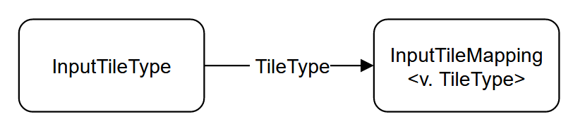
\includegraphics[scale=1]{img/relation-tiletype-tilemapping}
	\caption[Relation zwischen InputTileType und InputTileMapping]{Relation zwischen InputTileType und InputTileMapping\footnotemark}
\end{figure}
\footnotetext{eigene Darstellung}

Dabei haben sich zwei Use Cases herauskristallisiert:

Die Grundidee ist, dass alle in \code{TileMapping} definierten Kacheln eines bestimmten \code{TileTypes} dem Anwender zur Auswahl präsentiert werden. Diese werden dabei dynamisch aus der \code{TileMapping}-Klasse ausgelesen. Der passende \code{OnClickListener} wird mithilfe der \code{InputMenuFactory} gesetzt. Bei den Kacheltypen-Action und Einstellung wird lediglich die bearbeitete Kachel durch die neue, ausgewählte Kachel vom Typ \code{Action} oder Einstellung ersetzen. Bei der Eingabe eines Operanden wird jedoch ein weiteres Menü aufgerufen, welches dies handhabt. Erst nach erfolgreicher Eingabe kann die bearbeitete Kachel ersetzt werden.

\begin{figure}[h]
	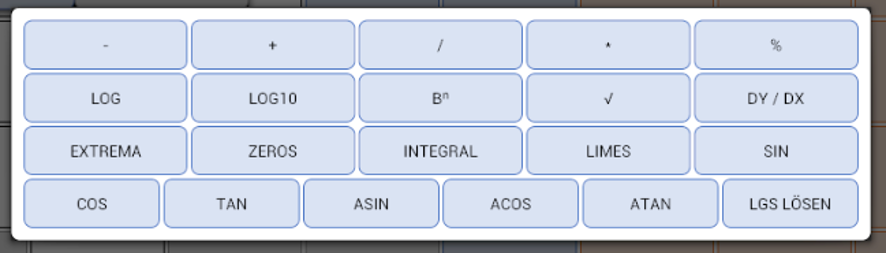
\includegraphics[width=\columnwidth]{img/inputtilemapping-for-operators}
	\caption[InputTileMapping for Operators]{InputTileMapping for Operators\footnotemark}
\end{figure}
\footnotetext{eigene Darstellung}

Im Kontrast zu den vielen Kacheldefinitionen, die es in \code{TileMapping} zu Einstellungen oder Operatoren gibt, findet man dort für den Stack und die Historie lediglich eine Definition wieder. (\code{S\_STACK}, \code{H\_HISTORY})

Was bei der Erstellung von sowohl Stack, als auch Historie von Relevanz ist, ist der Rang der Kachel. Dieser legt gemäß \code{TileScheme}-Definition fest, zu welchem Zeitpunkt Daten hineingeschoben oder gelöscht werden. Im \code{InputTileMapping} wird also für jeden möglichen Position in der Liste ein Eintrag angelegt. Gemäß der, vom \code{InputMenuFactory} erstellten Listener, wird dann das Historie- bzw. Stack-Tile an die ausgewählte Stelle gesetzt.

\begin{figure}[h]
	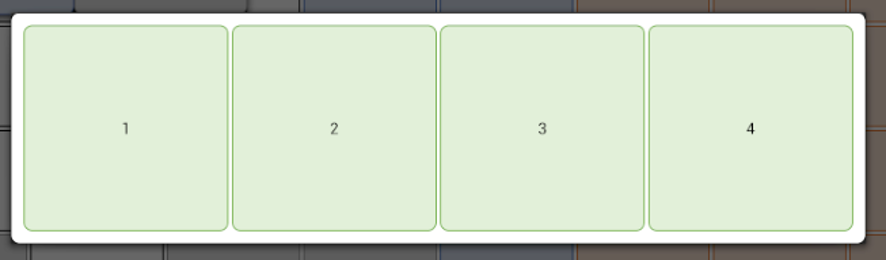
\includegraphics[width=0.7\columnwidth]{img/inputtilemapping-for-stack-with-3-tiles}
	\caption[InputTileMapping for Stack with 3 tiles]{InputTileMapping for Stack with 3 tiles\footnotemark}
\end{figure}
\footnotetext{eigene Darstellung}
\FloatBarrier

\paragraph{Klasse: InputDouble [Gentges]}

Für die Applikationen werden folgende Operanden (\code{ODouble}, \code{OFraction} und \code{OPolynom}) für die Eingabe vom User möglich sein. Die XML-Ansicht ist simpel gehalten und verwendet ein \code{RelativeLayout} hat, welches die relative Position zu den einzelnen Objekte verwendet. Dadurch wird die Layout-Hierarchie reduziert und die Performance der Applikation verbessert. Für das Eingabefeld wird ein \code{EditText} verwendet, das als Eingabetyp Dezimalzahlen unterstützt wird. In Android muss hier noch explizit erwähnt werden, dass erst über den Keyword \code{numberSigned} auch die Eingabe von negative Zahlen möglich ist.

\begin{figure}[h]
	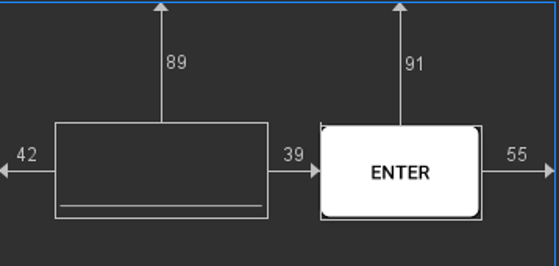
\includegraphics[width=0.6\columnwidth]{img/xml_InputDouble}
	\caption[XML-Designer für die Klassen InputDouble]{XML-Designer für die Klasse InputDouble\footnotemark}
\end{figure}
\footnotetext{eigene Darstellung}
\FloatBarrier

Die korrespondierende Java-Datei liest nach dem Bestätigen des Buttons den Wert aus dem \code{EditText} und kreiert ein \code{ODouble}-Objekt. Dieses Objekt wird mit seinem zugehörigen \code{TileMapping} einem \code{TileScheme} zugewiesen. Das vorher ausgewählte \code{Tile} aktualisiert seinen \code{TileScheme}. Abschließend schließt der Konstruktor die Dialog über die Methode \code{dismissAll()}, die vorher erklärt wurde.

\paragraph{Klasse: InputFraction [Gentges]}

Diese Klasse deckt die Funktionalität der Benutzereingabe von Brüchen. Dabei ähnelt sie der Klasse \code{InputDouble}. Die Unterschiede beruhen dahingehend, dass ein zweites \code{EditText} integriert wurde, um sowohl als Zähler als auch Nenner abzufragen. Der ausgewählten \code{Tile} wird respektiv ein \code{TileScheme} mit \code{OFraction} übergeben. 

\begin{figure}[h]
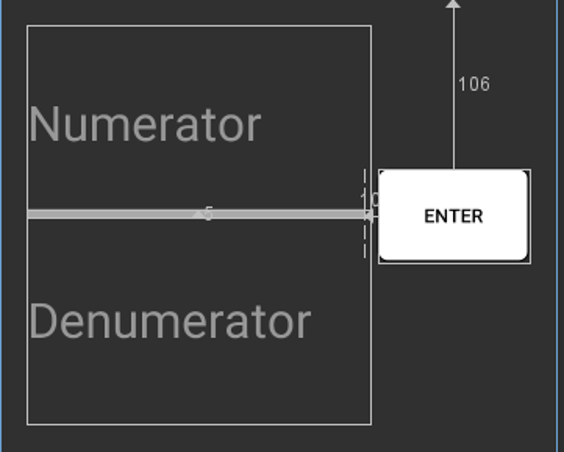
\includegraphics[width=0.5\columnwidth]{img/xml_InputFraction}
\caption[XML-Designer für die Klasse InputFraction]{XML-Designer für die Klasse InputFraction\footnotemark}
\end{figure}
\footnotetext{eigene Darstellung}
\FloatBarrier

\paragraph{Klasse: InputPolynomial [Gentges]}

Die Klasse ist grundsätzlich gleich aufgebaut, wie die vorherigen Eingabeklassen der Operanden. In der Abbildung lässt sich erkennen, dass die einzelne Polynome vom Nutzer eingegeben werden können.

\begin{figure}[h]
	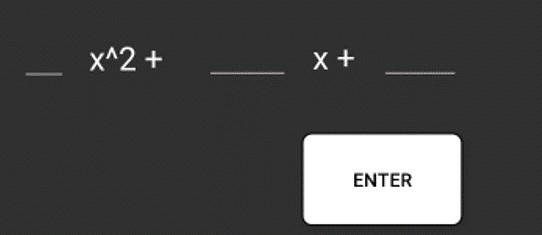
\includegraphics[width=0.6\columnwidth]{img/xml_InputPolynomial}
	\caption[XML-Designer für die Klasse InputPolynomial]{XML-Designer für die Klasse InputPolynomial\footnotemark}
\end{figure}
\footnotetext{eigene Darstellung}
\FloatBarrier

\paragraph{Darstellung der Beziehungen von den Menüsteuerungsklassen [Istogu]}

\begin{figure}[h]
	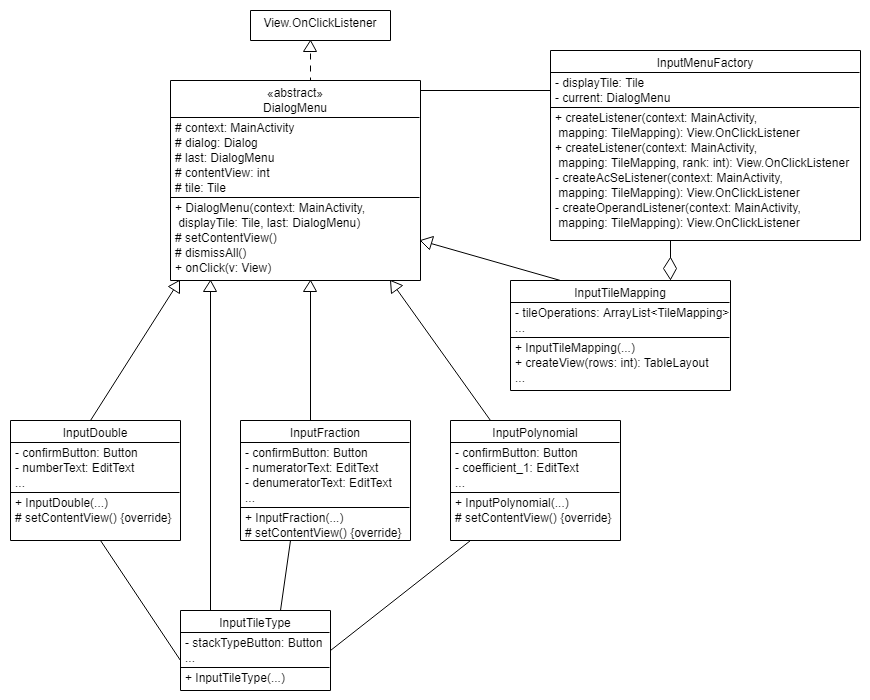
\includegraphics[width=\columnwidth]{img/klassendiagramm_Menusteuerung}
	\caption[Klassendiagramm: Menüsteuerung]{Klassendiagramm: Menüsteuerung\footnotemark}
\end{figure}

Wie aus dem Klassendiagramm entnommen werden kann, wurde die Menüsteuerung soweit wie möglich dynamisch gestaltet. Somit wird die Erweiterbarkeit vereinfacht und es können dadurch weitere Funktionalitäten bzgl. Operanden bzw. Operationen hinzugefügt werden. Zusätzlich sind die einzelne Menüs wie folgt gestaltet. Die einzelne Menüs bauen aufeinander und somit ist der Ablauf der einzelnen Menüs definiert. 
\clearpage

\subsection{Dokumentation der Models }

\subsubsection{Operanden [Schwenke]}

Für ein gut funktionierendes Backend ist ein einheitliches Datenmodel essenziell. So gibt es in der Kernbibliothek von Java einige Klassen für die Repräsentation von mathematischen Bausteinen, wie z.B. dem Bruch. Das gleiche gilt für \textit{Apache Commons Math}. 

Jedoch sind die meisten dieser Klassen sehr spezialisiert und miteinander nicht kompatibel. Deswegen wurde innerhalb des Projektteams entschieden für jeden unterstützten Operanden eine eigene Klasse zu entwickeln, die jedoch alle von der gleichen abstrakten Klasse \code{Operand} erben sollen. 

Dadurch wird sichergestellt, dass es eine einheitliche Schnittstelle gibt, über die alle Operanden angesprochen werden können. Beschreiben kann man diese neuen Klassen auch als \textit{Wrapper}, da der Großteil der eigentlichen Funktionalitäten Teil der darunterliegenden Klassen ist. 

So soll z.B. \code{OMatrix} ein Wrapper um die Klasse \code{Array2DRowRealMatrix} sein. Damit kann man einerseits das einfache und einheitliche Interface nutzen und falls notwendig direkt auf das darunterliegende Objekt zugreifen, um spezielle Operationen durchführen zu können. 

Ein wichtiger Bestandteil dieser Wrapper sind auch die unterschiedlichen Konstruktoren. So kann jeder Operand aus einem einzelnen String konstruiert werden. 

Im Folgenden wird die gemeinsame Schnittstelle dargestellt. Gemeinsam haben alle diese Methoden, dass sie ohne Seiteneffekte auskommen. Statt das vorliegende Objekt zu verändern wird ein neues Objekt erstellt und zurückgegeben. Dies macht das Umkehren von Methodenaufrufen einfach. Man muss lediglich das zurückgegebene Objekt entfernen und das alte weiternutzen.

\paragraph{Klasse: Operand [Schwenke]}

\code{Operand turnAroundSign()}: Dreht alle Vorzeichen im Operand um. Erreicht wird das grundsätzlich durch Multiplikation mit \code{-1}. Konkreter muss dafür z.B. bei einer Matrix eine Multiplikation mit einem Skalar durchgeführt werden.

\code{Operand negateValue()}: Negiert den Operanden unabhängig von den Vorzeichen. Bei einer Matrix werden also alle Elemente negativ.

\code{Operand inverseValue()}: Die Inverse (wenn vorhanden) des jeweiligen Operanden wird berechnet.

\code{Boolean equalsValue(Operand o)}: Vergleicht den aktuellen Operanden mit einem übergebenen Operanden.

\code{String toString()}: Wandelt das Objekt in eine String-Repräsentation um.

\code{<T extends Object> get()}: Gibt das darunterliegende Objekt zurück. Im Falle von \code{OMatrix} ist dies eine \code{Array2DRowRealMatrix}. Bei einem Tupel ein \code{Array} von \code{Doubles}.

Auffallend ist hier der geringe Umfang der Schnittstelle der Operanden, da diese doch eigentlich die Grundlage für einen Taschenrechner bilden sollten. So kann man eine Matrix multiplizieren, addieren, dividieren und das alles in unterschiedlichsten Kombinationen mit anderen Arten von Operanden. Tatsächlich sind die meisten Kalkulationen – wie in der Projektplanung entworfen – in eigenen Klassen angelegt. Somit besteht eine Trennung zwischen Datenhaltung (den Operanden) und den Operationen, die auf den Daten ausgeführt werden können (Actions).

\paragraph{Klasse: ODouble [Meinerzhagen]}

\textit{Wrapper für ein} \code{Double}

Eine Dezimalzahl, welche intern einen \code{double} zur Datenspeicherung verwendet.


\paragraph{Klasse: OFraction [Meinerzhagen]}

\textit{Wrapper für Common Math Fraction}

Implementierung eines Bruchs. Die Zähler und Nenner sind durch \code{Doubles} umgesetzt. Im Gegensatz zu den meisten anderen Operanden gibt es hier mehr als zwei Konstruktoren. So kann man einmal Zähler und Nenner als zwei ganze Zahlen übergeben. Wird ein einzelnes \code{Double} übergeben, wird daraus automatisch ein Bruch erstellt. Alternativ kann direkt eine \code{Fraction} übergeben werden.

\paragraph{Klasse: OSet [Meinerzhagen]}

\textit{Wrapper für ein} \code{Double}-\code{Set}

Implementierung einer Menge. Das gleiche Element kann nicht mehrmals enthalten sein. Die Reihenfolge spielt keine Rolle. Umgesetzt ist die Klasse mit einem angepassten \code{Set}. Erstellen kann man ein \code{OSet} aus einem \code{Array} von \code{Doubles} oder einem String.

\paragraph{Klasse: OTuple [Meinerzhagen]}

\textit{Wrapper für ein} \code{Double}-\code{Array}

Implementierung eines Tupels. Das gleiche Element kann mehrmals enthalten sein. Die Reihenfolge spielt eine Rolle. Erstellen kann man ein \code{OTuple} aus einer übergebenen Liste oder einem String.

\paragraph{Klasse: OMatrix [Meinerzhagen]}

\textit{Wrapper für eine Apache Commons} \code{Array2DRowRealMatrix}

Implementierung einer Matrix. Das darunterliegende Objekt ist eine \code{RealMatrix}, die wiederrum eine \code{Array2DRowRealMatrix} enthält. Die Matrix an sich ist in einem zweidimensionalen Array von \code{Doubles} umgesetzt. Erstellen kann man eine \code{OMatrix} aus einem String oder einem zweidimensionalen \code{Array} von \code{Doubles}.


\paragraph{Klasse: OPolynom [Meinerzhagen]}

\textit{Wrapper für eine Apache Commons} \code{PolynomialFunction}

Implementierung eines Polynoms. Grundsätzlich entspricht das Polynom einer einer Sequenz von Dezimalzahlen. Abhängig von der Position in der Sequenz entscheidet sich, was der Exponent der jeweiligen Dezimalzahl ist. Somit müssen Funktionen immer in dieser Normalform vorliegen. Erstellen kann man ein \code{OPolynom} aus einem String oder einem \code{Array} von \code{Doubles}.

\paragraph{Klasse: OEmpty [Meinerzhagen]}

\textit{Leerer Wrapper}

Ein leerer Operand. Da alle \code{Operand}-Klassen Wrapper sind, ist technisch auch ein leerer Wrapper notwendig. Die hier implementierten Methoden aus der Schnittstelle stellen lediglich \textit{Stubs} dar und haben keine Funktion.

\paragraph{Klasse: DoubleFormatter [Meinerzhagen]}

Zentrale Anlaufstelle um \code{Doubles} in einen formattierten String umzuwandeln. Die einzige hier enthaltene Methode ist 

\code{String format(double d)}

\paragraph{Klasse: DoubleComparator [Meinerzhagen]}

Dezimalzahlen sind in den meisten Sprachen in dem IEE 754 Format implementiert. Das hat zur Folge, dass Konversionen und Änderungen einer konkreten Dezimalzahl zu Rundungsfehlern führen. Das ist auch in Java der Fall. Möchte man nun die beiden Dezimalzahlen \code{1.1} und \code{1.1} mit der Standardmethode in Java vergleichen, wird man in fast allen Fällen ein \code{false} zurückbekommen. Das liegt an den zuvor angesprochenen Rundungsfehlern. 

Da innerhalb dieses Projekts alles auf \code{Doubles} basiert ist es notwendig für dieses Problem eine Lösung zu finden. Dafür wurde diese Klasse entwickelt. Alle Vergleiche müssen über diese Klasse erfolgen.

\code{Boolean isEqual(double d1, double d2)} vergleicht zwei \code{Doubles} miteinander. Dies erfolgt über ein Delta. Zunächst wird die Differenz zwischen beiden Zahlen berechnet und anschließend überprüft, ob die Differenz unter einer definierten Grenze liegt. Alle weiteren Methoden in dieser Klasse benutzen diese Methode.

Weitere Methoden vergleichen \code{Arrays} und \code{Sets} miteinander.

\subsubsection{Operationen}

\paragraph{Klasse: Plus [Falk]}

\textbf{Eingabeparameter: }Zwei Werte, der erste Wert ist der erste Summand, der zweite der zweite Summand. Die erlaubten Kombinationen sind: 

\begin{itemize}
	\item \code{ODouble} und \code{ODouble}
	\item \code{ODouble} und \code{OFraction}
	\item \code{OFraction} und \code{ODouble}
	\item \code{ODouble} und \code{OSet}
	\item \code{OSet} und \code{ODouble}
	\item \code{ODouble} und \code{OMatrix}
	\item \code{OMatrix} und \code{ODouble}
	\item \code{ODouble} und \code{OPolynom}
	\item \code{OPolynom} und \code{ODouble}
	\item \code{ODouble} und \code{OTupel}
	\item \code{OTupel} und \code{ODouble}
	\item \code{OFraction} und \code{OFraction}
	\item \code{OFraction} und \code{OSet}
	\item \code{OSet} und \code{OFraction}
	\item \code{OFraction} und \code{OMatrix}
	\item \code{OMatrix} und \code{OFraction}
	\item \code{OFraction} und \code{OPolynom}
	\item \code{OPolynom} und \code{OFraction}
	\item \code{OFraction} und \code{OTuple}
	\item \code{OTupel} und \code{OFraction}
	\item \code{OMatrix} und \code{OMatrix}
	\item \code{OPolynom} und \code{OPoylnom}
	\item \code{OTuple} und \code{OTuple}
\end{itemize}

\textbf{Rückgabewerte: }Der berechnete Wert mit dem Datentyp des ersten Summanden. 

\textbf{Beschreibung: }Die Klasse verfügt über 23 öffentlich ansprechbare Methoden. Je nach übergebenen Parametern wird bestimmt, welche öffentliche Methode gemeint ist. Anschließend wird die Berechnung durchgeführt. 

\paragraph{Klasse: Minus [Falk]}

\textbf{Eingabeparameter: }Zwei Werte, der erste Wert ist der Minuend, der zweite der Subtrahend. Die erlaubten Kombinationen sind: 

\begin{itemize}
	\item \code{ODouble} und \code{ODouble} 
	\item \code{ODouble} und \code{OFraction}
	\item \code{OFraction} und \code{OFraction} 
	\item \code{OFraction} und \code{ODouble}
	\item \code{OSet} und \code{ODouble}
	\item \code{OSet} und \code{OFraction }
	\item \code{OMatrix} und \code{OMatrix}
	\item \code{OMatrix} und \code{ODouble}
	\item \code{OMatrix} und \code{OFraction}
	\item \code{OPolynom} und \code{OPolynom }
	\item \code{OPolynom} und \code{ODouble}
	\item \code{OPolynom} und \code{OFraction }
	\item \code{OTuple} und \code{OTuple}
	\item \code{OTuple} und \code{ODouble}
	\item \code{OTuple} und \code{OFraction}
\end{itemize} 

\textbf{Rückgabewerte: }Der berechnete Wert mit dem Datentyp des ersten, übergebenen Wertes. 

\textbf{Beschreibung: }Die Klasse verfügt über 15 öffentlich ansprechbare Methoden. Je nach übergebenen Parametern wird bestimmt, welche öffentliche Methode gemeint ist. Anschließend wird die Berechnung durchgeführt. 

\paragraph{Klasse: Minus [Falk]}

\textbf{Eingabeparameter: }Zwei Werte, der erste Wert ist der Dividend, der zweite der Divisor. Die erlaubten Kombinationen sind: 

\begin{itemize}
	\item \code{ODouble} und \code{ODouble}
	\item \code{ODouble} und \code{OFraction}
	\item \code{OFraction} und \code{OFraction} 
	\item \code{OFraction} und \code{ODouble} 
	\item \code{OSet} und \code{ODouble}
	\item \code{OSet} und \code{OFraction}
	\item \code{OMatrix} und \code{ODouble}
	\item \code{OMatrix} und \code{OFraction}
	\item \code{OPolynom} und \code{OPolynom}
	\item \code{OPolynom} und \code{ODouble}
	\item \code{OPolynom} und \code{OFraction}
	\item \code{OTuple} und \code{OTuple}
	\item \code{OTuple} und \code{ODouble}
	\item \code{OTuple} und \code{OFraction} 
\end{itemize}

\textbf{Rückgabewerte:} Der berechnete Wert mit dem Datentyp des ersten, übergebenen Wertes.
 
\textbf{Beschreibung: }Die Klasse verfügt über 14 öffentlich ansprechbare Methoden. Je nach übergebenen Parametern wird bestimmt, welche öffentliche Methode gemeint ist. Bevor die Berechnung durchgeführt wird, wird bestimmt ob der Divisor \code{0} ist. Wenn ja wird eine Fehlermeldung ausgegeben. Andernfalls wird die Berechnung durchgeführt. 

\paragraph{Klasse: Times [Falk]}

\textbf{Eingabeparameter:} Zwei Werte, der erste Wert ist der Multiplikator, der zweite Wert der Multiplikand. Die erlaubten Kombinationen sind: 

\begin{itemize}
\item \code{ODouble} und \code{ODouble}
\item \code{ODouble} und \code{OFraction}
\item \code{OFraction} und \code{ODouble}
\item \code{ODouble} und \code{OSet}
\item \code{OSet} und \code{ODouble}
\item \code{ODouble} und \code{OMatrix}
\item \code{OMatrix} und \code{ODouble}
\item \code{ODouble} und \code{OPolynom}
\item \code{OPolynom} und \code{ODouble}
\item \code{ODouble} und \code{OTupel}
\item \code{OTupel} und \code{ODouble}
\item \code{OFraction} und \code{OFraction}
\item \code{OFraction} und \code{OSet}
\item \code{OFraction} und \code{OMatrix}
\item \code{OMatrix} und \code{OFraction}
\item \code{OFraction} und \code{OPolynom}
\item \code{OFraction} und \code{OTupel}
\item \code{OMatrix} und \code{OMatrix}
\item \code{OPolynom} und \code{OPolynom} 
\item \code{OTupel} und \code{OTupel}
\end{itemize}

\textbf{Rückgabewerte: }Der berechnete Wert. 

\textbf{Beschreibung: }Die Klasse verfügt über 20 öffentlich ansprechbare Methoden. Je nach übergebenen Parametern wird bestimmt, welche öffentliche Methode gemeint ist. Anschließend wird die Berechnung durchgeführt. 

\paragraph{Klasse: Root [Falk]}

\textbf{Eingabeparameter: }Zwei Werte, der erste Wert ist der Radikand, der zweite Wert der Wurzelexponent. Die erlaubten Kombinationen sind: 

\begin{itemize}
\item \code{ODouble} und \code{ODouble}
\item \code{ODouble} und \code{OFraction}
\item \code{OFraction} und \code{ODouble} 
\item \code{OFraction} und \code{OFraction}
\item \code{OMatrix} und \code{ODouble}
\item \code{OMatrix} und \code{OFraction}
\end{itemize}

\textbf{Rückgabewerte:} Der berechnete Wert, Datentyp ist der des Radikanden. 

\textbf{Beschreibung: }Die Klasse verfügt über 6 öffentliche Methoden. Anhand der übergebenen Parameter wird bestimmt, welche öffentliche Methode aufgerufen wird. In der Methode wird die Wurzel berechnet und zurückgegeben. 

\paragraph{Klasse: Modulo [Falk]}

\textbf{Eingabeparameter:} Zwei Werte des Typs \code{ODouble}, der erste Wert ist der Dividend, der zweite der Divisor. 

\textbf{Rückgabewerte:} Der berechnete Wert als \code{ODouble}. 

\textbf{Beschreibung:} Die Klasse verfügt über eine öffentliche Methode. In der Methode wird der Modulo-Wert der beiden übergebenen Parameter berechnet. 

\paragraph{Klasse: Zeros [Keienburg]}

\textbf{Eingabeparameter: }Eine Funktion des Typs \code{OPolynom}

\textbf{Rückgabewerte:} Ein Set des Typs \code{OSet} mit den berechneten Nullstellen. Die Nullstellen werden als \code{Set} zurückgegeben, da so verhindert wird das für Funktionen wie \code{x\^{}2+0*x+0} zweimal die gleiche Nullstelle zurückgegeben wird. 

\textbf{Einstieg in die Klasse:} Öffentliche Methode, die die übergebenen Parameter entgegennimmt. Die weiteren Methoden für die Berechnung werden anschließend von der Öffentlichen Methode aus aufgerufen. 
Methoden der Klasse \code{Zeros}:

\code{calculateZeros}: Die Methode erhält eine Funktion vom Typ \code{OPolynom}. Anschließend wird bestimmt, von welchem Grad die übergebene Funktion ist. Wenn die Funktion ersten Grades ist, wird die Methode \code{zerosTypeOne} aufgerufen, ansonsten die Methode \code{zerosTypeTwo}. Die beiden Methoden geben die gefundenen Nullstellen als 
Array zurück, das Array wird anschließend von \code{calculateZeros} zurückgegeben.
 
\code{normalOrQuadraticFunction}: Bestimmt, ob eine, als \code{Double} Array übergebene Funktion, ersten oder zweiten Grades ist. Dabei wird die Länge des Arrays getestet. Ist die Länge des Arrays 3, so wird die Funktion als Quadratische Funktion bestimmt. Wenn die Länge 2 ist, als einfache Funktion. 

\code{zerosTypeOne}: Die Methode berechnet die Nullstellen für Funktionen ersten Grades. Die Funktion wird als Double Array übergeben. Die berechnete Nullstelle wird als Double Array zurückgegeben. 

\code{zerosTypeTwo}: Die Methode berechnet die Nullstellen für Funktionen zweiten Grades. Die Funktion wird als Double Array übergeben. Mithilfe der Mitternachtsformel wird die erste und die zweite Nullstelle bestimmt. Die gefundenen Nullstellen werden als Double Array zurückgegeben. 

\textbf{Anmerkung:} Wenn eine übergebene Funktion keine Nullstellen besitzt, der Rückgabewert in Java also \code{NaN} ist, wird eine Fehlermeldung ausgegeben, dass eine Nullstellenberechnung nicht möglich ist. 

\textbf{Einschränkungen:} Die Nullstellenberechnung ist nur für Funktionen ersten und zweiten Grades möglich. 

Unit-Tests für die Klasse: 

\begin{enumerate}
	\item Eingabe Funktion: \code{2x + 4}. Erwartetes Ergebnis: \code{(-2)}
	\item Eingabe Funktion: \code{2x\^{}2+4x+0}. Erwartetes Ergebnis: \code{(-2, 0)}
	\item Eingabe Funktion: \code{x\^{}2+4x-4}. Erwartetes Ergebnis: \code{(-4,828, 0,828)}
\end{enumerate}

Die Tests waren erfolgreich.

\paragraph{Klasse: HighAndLowPoints [Keienburg]}

\textbf{Eingabeparameter:} Eine Funktion des Typs \code{OPolynom}

\textbf{Rückgabewerte: }Ein Tupel des Typs \code{OTupel} mit den berechneten Extremwerten. Die Werte an den geraden Positionen innerhalb des Tupels sind die X-Werte, der jeweils folgende Wert ist der zugehörige Y-Wert. Bsp.: Tupel [0] = X-Wert des ersten Extremwertes, Tupel [1] = Y-Wert des ersten Extremwertes, Tupel [2] = X-Wert des zweiten Extremwertes, Tupel [3] = Y-Wert des zweiten Extremwertes. 

Beschreibung: Die Klasse erhält eine Funktion vom Typ \code{ODouble}. Zuerst wird die Ableitung der Funktion bestimmt, anschließend die Nullstellen der Abteilung. Für die erhaltenen Nullstellen wird der zugehörige Y-Wert berechnet. Die berechneten Werte werden als \code{OTupel} zurückgegeben. 

Einstieg in die Klasse: Öffentliche Methode, die die übergebenen Parameter entgegennimmt. Die weiteren Methoden für die Berechnung werden anschließend von der Öffentlichen Methode aus aufgerufen. 

\textbf{Methoden der Klasse \code{HighAndLowPoints}:}

\code{getHighAndLowPoints}: Einstiegspunkt der Klasse, ruft die Methode \code{calculate}\linebreak\code{HighAndLowPoints} für die weitere Berechnung der Extremwerte auf. Gibt sie als \code{Double}-\code{Array} zurück. 

\code{getFunctionAsDouble}: Wandelt eine übergebene Funktion vom Typ \code{OPolynom} in ein Double Array um.

\code{calculateHighAndLowPoints}: Berechnet die Nullstellen einer übergebenen Funktion vom Typ \code{OPolynom}. Berechnet zuerst die Ableitung der Funktion, anschließend die Nullstellen der Ableitung. Die Werte der Nullstellen werden anschließend in die ursprüngliche Funktion eingesetzt und so die Y-Werte berechnet. Die berechneten Nullstellen werden als Double Array zurückgegeben. 

\code{Einschränkungen}: Die Nullstellenberechnung ist nur für Funktionen zweiten Grades möglich. Demnach ist eine Berechnung der Hoch- und Tiefpunkte nur für Funktionen dritten oder zweiten Grades möglich.

Unit-Tests für die Klasse:

\begin{enumerate}
\item Eingabe Funktion: 2x\^{}2+4x+6. Erwartetes Ergebnis: (-1|4)
\item Eingabe Funktion: 3x\^{}2+6x-4. Erwartetes Ergebnis: (-1|-7)
\item Eingabe Funktion: -2*x\^{}2+4x+12. Erwartetes Ergebnis: (1|14)
\end{enumerate}

Die Tests waren erfolgreich.

\paragraph{Logarithm [Keienburg]}

\textbf{Eingabeparameter:} Ein Wert des Typs \code{ODouble} oder zwei Werte vom Typ \code{ODouble} (erster ist die Basis) 

\textbf{Rückgabewerte:} Ein Wert des Typs \code{ODouble}

\textbf{Beschreibung:} Die Klasse berechnet den Logarithmus. Die Art des Logarithmus ist abhängig von den übergebenen Parametern. Wird nur ein Wert übergeben, wird der natürliche Logarithmus der Zahl berechnet. Wenn zwei Parameter übergeben werden, ist der erste Parameter die Basis des Logarithmus, der zweite der Wert, zu für den der Logarithmus berechnet werden soll. 

Der Einstieg in die Klasse erfolgt über zwei öffentliche Methoden. Die Methode wird anhand der übergebenen Parameter (ein oder zwei Werte vom Typ \code{ODouble}) ausgewählt. In der Öffentlichen Methode findet die Berechnung des Logarithmus (Natürlicher oder Logarithmus zu einer bestimmten Basis) statt. Wenn ein Wert kleiner gleich null eingegeben wird, wird eine Fehlermeldung ausgegeben.

Unit-Tests für die Klasse: 4 Unit-Test für die Berechnung der des natürlichen Logarithmus (ersten 4), 3 Unit-Tests für die Berechnung des Logarithmus für eine beliebige Basis. 

\begin{enumerate}
\item Eingabe 10. Erwartetes Ergebnis: 2.302585092994046
\item Eingabe: 5. Erwartetes Ergebnis: 1.6094379124341003
\item Eingabe: 97. Erwartetes Ergebnis: 4.574710978503383
\item Eingabe: e. Erwartetes Ergebnis: 1
\item Eingabe: Basis 5, Wert 10. Erwartetes Ergebnis: 1.4306765580733933
\item Eingabe: Basis 10, Wert 10. Erwartetes Ergebnis: 1
\item Eingabe: Basis e, Wert 10. Erwartetes Ergebnis: 2.302585092994046
\end{enumerate}

Die Tests waren erfolgreich.

\paragraph{Logarithm10 [Keienburg]}

\textbf{Eingabeparameter:} Ein Wert des Typs \code{ODouble}

\textbf{Ausgabeparameter:} Ein Wert des Typs \code{ODouble}

\textbf{Beschreibung:} Die Klasse berechnet den Logarithmus zur Basis 10. Wenn ein Wert kleiner gleich 0 eingegeben wird, wird eine Fehlermeldung ausgegeben. 

Unit-Tests für die Klasse: 

\begin{enumerate}
\item Eingabe 10. Erwartetes Ergebnis: 1
\item Eingabe: 5. Erwartetes Ergebnis: 0.6989700043360189
\item Eingabe: 97. Erwartetes Ergebnis: 1.9867717342662448
\end{enumerate}

Die Tests waren erfolgreich.

\paragraph{Derivation [Keienburg]}

\textbf{Eingabeparameter: }Eine Funktion des Typs \code{OPolynom}

\textbf{Rückgabewert:} Eine Funktion des Typs \code{OPolynom}

\textbf{Beschreibung:} Die Klasse berechnet die Ableitung zu einer übergebenen Funktion des Typs \code{OPolynom} und gibt sie als Funktion vom Typ \code{OPolynom} zurück. 

\textbf{Einstieg in die Klasse: }Öffentliche Methode, die die übergebenen Parameter entgegennimmt. Die weiteren Methoden für die Berechnung werden anschließend von der Öffentlichen Methode aus aufgerufen. 

\textbf{Methoden der Klasse Derivation: }

\code{getFunctionAsDouble:} Wandelt eine gegebene Funktion vom Typ \code{OPolynom} in ein \code{Double}-\code{Array} um. 

\code{derivate: }Berechnet die Ableitung einer gegebenen Funktion. Die Funktion wird zuerst in ein \code{Double}-\code{Array} umgewandelt, anschließend abgeleitet und als Funktion vom Typ \code{OPolynom} zurückgegeben. 

Unit-Tests für die Klasse: 

\begin{enumerate}
\item Eingabe 2x\^{}2+4x+6. Erwartetes Ergebnis: 4x+4
\item Eingabe: 7x+9. Erwartetes Ergebnis: 7
\item Eingabe: 12x\^{}2-3+12. Erwartetes Ergebnis: 24x-1
\item Eingabe: 1.5x\^{}2+2x+7. Erwartetes Ergebnis: 2.25x+2
\end{enumerate}  

Die Tests waren erfolgreich.

\paragraph{Integral [Istogu]}

Diese Klasse erbt von der Klasse \code{Action}. Daher sind die Methoden \code{with() }bereits implementiert. Diese Klasse berechnet entweder die Stammfunktion von dem übergebene Polynomialfunktion oder das Integral der Funktion. 

Für die Bildung der Stammfunktion benötigt die Methode \code{getAntiderivative()} eine \code{OPolynom} und gibt die Stammfunktion als Typ \code{OPolynom} zurück. Beim Aufleiten entsteht eine Konstante, die jede Wert annehmen kann. In der App wird festgelegt, dass diese Konstante immer 0 ist. Zweck hinter der Definition ist, dass mit dem \code{OPolynom} weitergerechnet werden kann, da diese nicht mit weiteren Variablen arbeiten kann.

Für das Berechnen des Integrals \code{getSimpsonIntegrator()} werden folgende Parametertypen erwartet: 

\begin{itemize}
	\item \code{OPolynom oPolynom}
	\item \code{double lowerBound}
	\item \code{double upperBound}
\end{itemize}

Das Integral für den vorgegebenen Bereich wird als \code{ODouble} zurückgegeben. Diese Methode realisiert die Simpsonregel für die Integration von realen Funktionen, die in dem genutzten Mathebibliothek als Klasse \code{SimpsonIntegrator} implementiert wurde. 

Nach der Implementierung der Klasse erstellte ich dazu gehörig eine Unit-Test-Klasse. Im Nachfolgenden werden die Ergebnisse dargestellt, die alle erfolgreich waren. 

\code{getSimpsonsIntegrator()}

\quad \quad \textbf{ Eingabe:} \code{OPolynom}: \code{x\^{}2 – 8x + 17}, untere Grenze: 2, obere Grenze 5

\quad \quad \textbf{Erwartetes Ergebnis:} 6

\code{getAntiderivative()}

\quad \quad \textbf{Eingabe:} \code{OPolynom}: \code{-3,21x\^{}3 + 3x + 7}

\quad \quad \textbf{Erwartetes Ergebnis}: \code{OPolynom}: \code{-0,8025x\^{}4 + 1,5x\^{}2 + 7x + c}

\vspace{1em}

\paragraph{Bestimmung des Grenzwertes einer Funktion [Istogu]}

Für die Umsetzung wurde die Funktion \code{value(double x)} der Klasse \code{PolynomialFunction} verwendet, die aus der Mathebibliothek \textit{Apache Commons Math} hervorgeht. Zudem bietet die \code{Double}-Klasse die Repräsentierung von positiv und negativ Unendlich an, die auch für die Methoden verwendet wurde.

Für die Bestimmung des Grenzwertes wurde sich an der Methode der numerischen Annäherung orientiert. Hierbei wird der Grenzwert durch die Annäherung von links und rechts des untersuchten Punktes bestimmt. Daher wurde die Anforderung in drei Methoden untergliedert, einmal die Methode \code{limitFromBelow(…)} und \code{limitFromAbove(…)}, die jeweils die Annäherung von verschiedenen Richtung bestimmt. Die Rückgabewerte der beiden Methoden werden in der Methode \code{limit(…)} miteinander verglichen. Zweck der Vergleichsabfrage ist es Definitionslücken abzufangen. Als Beispiel wird folgende Funktion angenommen:

\code{f(x)=1/x}

\begin{figure}[!h]
	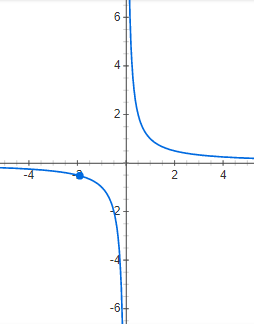
\includegraphics[scale=1]{img/funktion-grafik}
	\caption[Grafische Darstellung der Funktion]{Grafische Darstellung der Funktion\footnotemark}
\end{figure}
\footnotetext{eigene Darstellung}

Wenn für die Funktion sowohl der linksseitige als auch der rechtsseitige Grenzwert bestimmt wird, folgt folgendes:  

\begin{figure}[!h]
	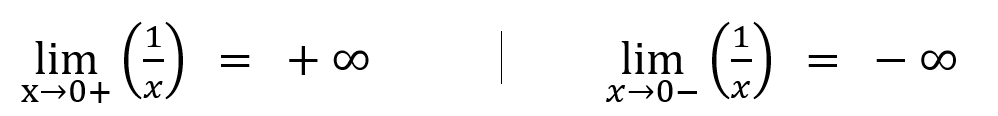
\includegraphics[width=\columnwidth]{img/limes-funktionen}
	\caption[Limes Funktion]{Limes Funktion\footnotemark}
\end{figure}
\footnotetext{eigene Darstellung}

Wenn der linksseitige und rechtsseitige Grenzwert nicht übereinstimmen, ist der Grenzwert an dieser Stelle nicht existent. In dem Fall beruht es darauf, dass das Ergebnis einer Division mit dem Divisor null nicht definiert ist. Solche Unstimmigkeiten können unter anderem auch in abschnittsweisen definierten Funktionen vorkommen, die im Funktionsumfang der App nicht integriert sind. Trotz dessen werden solche Fälle mit dem Vergleich zwischen dem linksseitigen und rechtsseitigen Grenzwert in der Methode \code{limit(…)} berücksichtigt.

Für die jeweilige Annäherung wurde die Überlegung getätigt, welche Fälle in der Grenzwertbestimmung von Funktionen vorkommen können. Dabei wurden folgende Lösungsmöglichkeiten festgestellt:
\begin{itemize}
	\item Positive unendlich
	\item Negativ unendlich
	\item Nicht definiert
	\item \code{xxx} war Zeichen (Ubiquator Teilmenge von Realer Zahlenraum)
\end{itemize}

Darauf aufbauend wurde ein Struktogramm angefertigt, auch als Nassi-Shneiderman-Diagramm bekannt. Dabei wird die Annäherung von unten veranschaulicht, weil die Annäherung von oben nach dem gleichen Grundprinzip erfolgt. 

\begin{figure}[!h]
	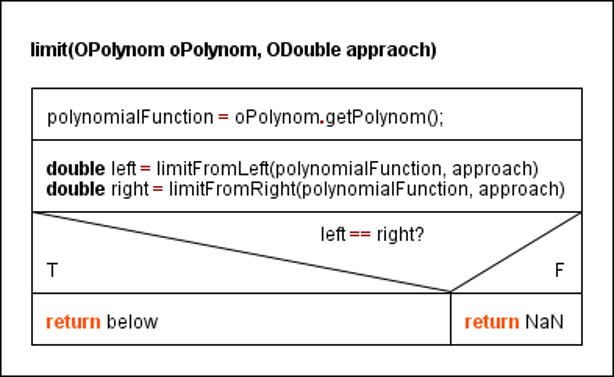
\includegraphics[scale=1]{img/struktogramm-limit}
	\caption[Struktogramm für die Methode limit]{Struktogramm für die Methode limit\footnotemark}
\end{figure}
\footnotetext{eigene Darstellung}


\begin{figure}[!h]
	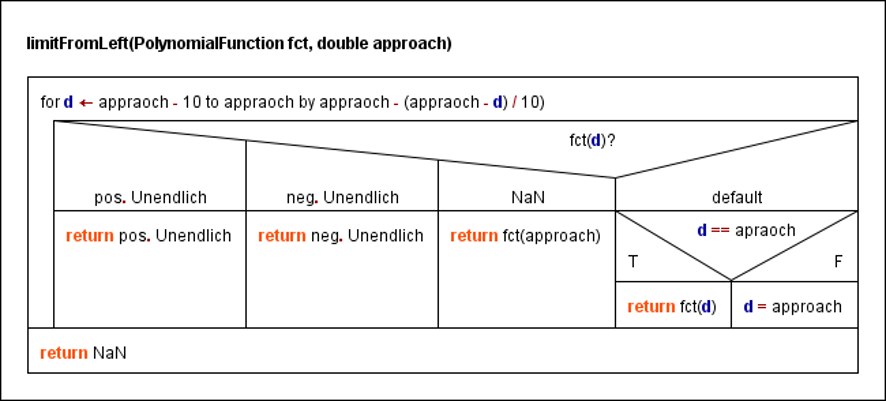
\includegraphics[scale=1]{img/struktogramm-limitFromLeft}
	\caption[Struktogramm für die Methode limitFromLeft]{Struktogramm für die Methode limitFromLeft\footnotemark}
\end{figure}
\footnotetext{eigene Darstellung}
\FloatBarrier

Die Klasse \code{Limes} erbt von der Klasse \code{Action}. Dahin gehend besitzt die Klasse die Methode \code{with()}, welche die Methode \code{on()} aufruft. Da diese Klasse keine Methodenüberladung für \code{on()} hat, wird kein Nutzen durch diese Art der Implementierung gewonnen, jedoch bietet es die Möglichkeit der Erweiterung an. In der Methode \code{on()} wird die Methode \code{limit()} aufgerufen.

\textbf{Methode:} \code{on()}

\textbf{Eingabeparameter: }Objekt des Typs \code{OPolynom}, Wert (Stelle an der, der Grenzwert berechnet wird) des Typs \code{ODouble}

\textbf{Rückgabewerte: }Einzelner Wert des Typs \code{ODouble}

Nach der Implementierung der Klasse erstellte ich dazu gehörig eine Unit-Test-Klasse. Im Nachfolgenden werden die Ergebnisse dargestellt, die alle erfolgreich waren.

\begin{enumerate}
	\item Eingabe: \code{OPolynom}: x\^{}2 + 1, Stelle: 26 \\
	Erwartetes Ergebnis: 26 
	\item Eingabe: -0.3333x\^{}3 + 2x, Stelle: pos. Unendlich \\
	Erwartetes Ergebnis: neg. Unendlich
	\item Eingabe: 3x\^{}3, Stelle: pos. Unendlich \\
	Erwartetes Ergebnis: pos. Unendlich
\end{enumerate}

\paragraph{Klasse: Sinus [Keienburg]}
\textbf{Eingabeparameter: } Einzelner Wert des Typs ODouble

\textbf{Rückgabewerte: } Einzelner Wert des Typs ODouble

\textbf{Beschreibung: } Der Klasse wird ein Winkel vom Datentyp ODouble übergeben. Der Winkel wird in einen Wert des Typs Double konvertiert, anschließend mithilfe der Methode Math.toRadians in ein Winkelmaß. Von diesem Winkelmaß wird dann mit der Methode Math.sin der Sinus berechnet und als ODouble zurückgegeben.  

Die Klasse wird über eine Öffentliche Methode aufgerufen. In der Methode selbst wird der Sinus berechnet. 

Unit-Tests für die Klasse: 	
\begin{enumerate}
	\item Eingabe:  10 Erwartetes Ergebnis: 0.17364817766693033
	\item Eingabe:  45 Erwartetes Ergebnis: 0.7071067811865475
	\item Eingabe: -45 Erwartetes Ergebnis: -0.7071067811865475
\end{enumerate}
Die Tests waren erfolgreich.

\paragraph{Klasse: ArcSinus [Keienburg]}
\textbf{Eingabeparameter: } Einzelner Wert des Typs ODouble

\textbf{Rückgabewerte: } Einzelner Wert des Typs ODouble

\textbf{Beschreibung: } Der Klasse wird ein Winkel vom Datentyp ODouble übergeben. Der Winkel wird in einen Wert des Typs Double konvertiert, anschließend mithilfe der Methode Math.toRadians in ein Winkelmaß. Von diesem Winkelmaß wird dann mit der Methode Math.asin die Inverse des Sinus berechnet und als ODouble zurückgegeben.  

Die Klasse wird über eine Öffentliche Methode aufgerufen. In der Methode selbst wird der Arkussinus berechnet. 

Unit-Tests für die Klasse: 	
\begin{enumerate}
	\item Eingabe:  10 Erwartetes Ergebnis: 0.17543139267904395
	\item Eingabe:  45 Erwartetes Ergebnis: 0.9033391107665127
	\item Eingabe: -45 Erwartetes Ergebnis: -0.9033391107665127
\end{enumerate}
Die Tests waren erfolgreich.

\paragraph{Klasse: Cosinus [Keienburg]}
\textbf{Eingabeparameter: } Einzelner Wert des Typs ODouble
	
\textbf{Rückgabewerte: } Einzelner Wert des Typs ODouble
	
\textbf{Beschreibung: } Der Klasse wird ein Winkel vom Datentyp ODouble übergeben. Der Winkel wird in einen Wert des Typs Double konvertiert, anschließend mithilfe der Methode Math.toRadians in ein Winkelmaß. Von diesem Winkelmaß wird dann mit der Methode Math.cos der Cosinus berechnet und als ODouble zurückgegeben.  Die Klasse wird über eine Öffentliche Methode aufgerufen. In der Methode selbst wird der Cosinus berechnet. 
	
Unit-Tests für die Klasse: 	
\begin{enumerate}
	\item Eingabe:  10 Erwartetes Ergebnis: 0.984807753012208
	\item Eingabe:  45 Erwartetes Ergebnis: 0.7071067811865476
	\item Eingabe: -45 Erwartetes Ergebnis: -0.7071067811865476
\end{enumerate}
Die Tests waren erfolgreich.

\paragraph{Klasse: ArcCosinus [Keienburg]}
\textbf{Eingabeparameter: } Einzelner Wert des Typs ODouble

\textbf{Rückgabewerte: } Einzelner Wert des Typs ODouble

\textbf{Beschreibung: } Der Klasse wird ein Winkel vom Datentyp ODouble übergeben. Der Winkel wird in einen Wert des Typs Double konvertiert, anschließend mithilfe der Methode Math.toRadians in ein Winkelmaß. Von diesem Winkelmaß wird dann mit der Methode Math.acos die Inverse des Cosinus berechnet und als ODouble zurückgegeben.  

Die Klasse wird über eine Öffentliche Methode aufgerufen. In der Methode selbst wird der Arkuscosinus berechnet. 

Unit-Tests für die Klasse: 	
\begin{enumerate}
	\item Eingabe:  10 Erwartetes Ergebnis: 1.3953649341158527
	\item Eingabe:  45 Erwartetes Ergebnis: 0.6674572160283838
	\item Eingabe: -45 Erwartetes Ergebnis: 2.4741354375614093
\end{enumerate}
Die Tests waren erfolgreich.

\paragraph{Klasse: Tangens [Keienburg]}
\textbf{Eingabeparameter: } Einzelner Wert des Typs ODouble

\textbf{Rückgabewerte: } Einzelner Wert des Typs ODouble

\textbf{Beschreibung: } Der Klasse wird ein Winkel vom Datentyp ODouble übergeben. Der Winkel wird in einen Wert des Typs Double konvertiert, anschließend mithilfe der Methode \code{Math.toRadians} in ein Winkelmaß. Von diesem Winkelmaß wird dann mit der Methode Math.tan der Tangens berechnet und als ODouble zurückgegeben.  

Die Klasse wird über eine Öffentliche Methode aufgerufen. In der Methode selbst wird der Tangens berechnet. 

Unit-Tests für die Klasse: 	
\begin{enumerate}
	\item Eingabe:  10 Erwartetes Ergebnis: 0.17632698070846498
	\item Eingabe:  45 Erwartetes Ergebnis: 0.9999999999999999
	\item Eingabe: -45 Erwartetes Ergebnis -0.9999999999999999
\end{enumerate}
Die Tests waren erfolgreich.

\paragraph{Klasse: ArcTangens [Keienburg]}
\textbf{Eingabeparameter: } Einzelner Wert des Typs ODouble

\textbf{Rückgabewerte: } Einzelner Wert des Typs ODouble

\textbf{Beschreibung: }Der Klasse wird ein Winkel vom Datentyp ODouble übergeben. Der Winkel wird in einen Wert des Typs Double konvertiert, anschließend mithilfe der Methode \code{Math.toRadians} in ein Winkelmaß. Von diesem Winkelmaß wird dann mit der Methode \code{Math.atan} die Inverse des Tangens berechnet und als ODouble zurückgegeben. 
 
Die Klasse wird über eine Öffentliche Methode aufgerufen. In der Methode selbst wird der Arkustangens berechnet. 

Unit-Tests für die Klasse: 	
\begin{enumerate}
	\item Eingabe:  10 Erwartetes Ergebnis: 0.1727924348551592
	\item Eingabe:  45 Erwartetes Ergebnis: 0.6657737500283538
	\item Eingabe: -45 Erwartetes Ergebnis: -0.6657737500283538
\end{enumerate}
Die Tests waren erfolgreich.

\subsubsection{Lösen von Gleichungssystemen [Istogu]}

Da bereits die Grundrechenoperationen auch den Operand Matrix unterstützt, beschäftigt sich die Klasse „MatrixUtil“ mit der Problemstellung ein lineares Gleichungssystem, die wie folgt aufgebaut ist…

\begin{figure}[h]
	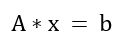
\includegraphics[scale=1]{img/gleichungssystem-loesen}
	\caption[Aufbau lineares Gleichungssystem]{Aufbau lineares Gleichungssystem\footnotemark}
\end{figure}

lösen. Dabei ist A eine quadratische Matrix (n x n) und b ein Vektor (n).
Die Klasse besitzt eine „on“ Methode, die dann solveLinearSystem() aufruft. Dabei erwartet die Methode „on“ jeweils ein Objekt des Typs OMatrix und OTuple und gibt ein OTuple zurück. 

\begin{figure}[h]
	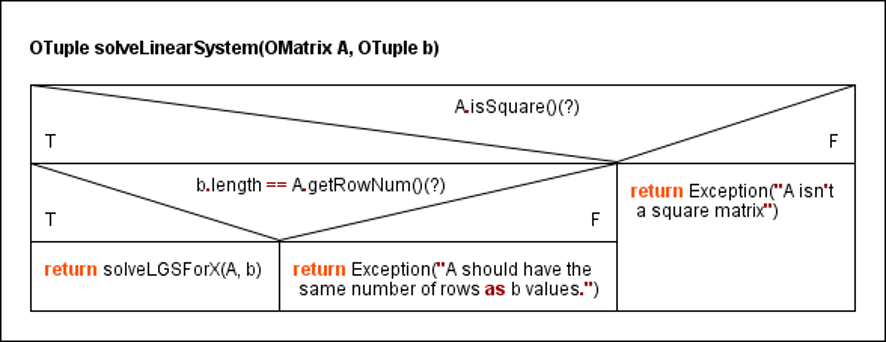
\includegraphics[width=\columnwidth]{img/solveLinearSystem}
	\caption[Struktogramm für die Methode solveLinearSystem]{Struktogramm für die Methode solveLinearSystem\footnotemark}
\end{figure}

Aus der Abbildung geht die geplante bzw. realisierte Umsetzung für die Überprüfung der Parameter nach ihrer richtigen Form. 

Nach der Implementierung der Klasse erstellte ich dazu gehörig eine Unit-Test-Klasse. Im Nachfolgenden werden die Ergebnisse dargestellt, die alle erfolgreich waren. 
\begin{enumerate}
	\item Eingabe: Matrix: xxx  Vektor: xxx Erwartetes Ergebnis: xxx
	\item Eingabe: Matrix: xxx Vektor: xxx Erwartetes Ergebnis: xxx
\end{enumerate}


\subsubsection{Stackhandhabung [Keienburg]}

Ein integraler Bestandteil eines RPN-Taschenrechners stellt der Stack für die Haltung der Operanden dar. Im Rahmen der Projektplanung ist festgestellt worden, dass die in Java vorhandenen Implementationen eines Stacks die Anforderungen des Projekts nicht erfüllen. Gesondert genannt werden soll hier nochmals die Möglichkeit mit einer beliebigen Anzahl von Objekten auf dem Stack gleichzeitig zu arbeiten. Aufgrund dessen wurde entschieden eine eigene Umsetzung eines Stacks zu entwickeln. Der Entwurf des neuen Stacks erfolgte mithilfe der Java-Schnittstelle \code{StackInterface}, welche im Folgenden (leicht vereinfacht) dargestellt ist.
void push(T value);
void push(T[] values);


T pop();\\
List<T> pop(int max);\\
<G extends T> G pop(Class<G> type);\\
<G extends T> List<G> pop(int max, Class<G> type);\\
T peek();\\
List<T> peek(int max); \\
<G extends T> G peek(Class<G> type); \\
<G extends T> List<G> peek(int max, Class<G> type); \\
boolean contains(T object); \\
void clear(); \\
T[] get(); \\
<G extends T> List<G> get(Class<G> type);\\
int size();

\code{T} und \code{G} werden in dem Interface als generische Typparameter genutzt. Das macht es möglich das Interface bzw. den Stack mit verschiedensten Implementationen zu nutzen. So kann man bei Bedarf nicht nur die einen Stack für Operanden, sondern auch für andere Klassen implementieren. Bei der Implementation wird der Typ-Paramter \code{T} durch eine konkrete Klasse (z.B. \code{Operand}, ersetzt. Ein Neuentwurf der Schnittstelle ist nicht notwendig. 

Der größte Unterschied zu anderen Stack-Interfaces ist, dass die drei bekannten Stack-Operationen push, pop und peek sowohl einzelne Parameter als auch Sammlungen von Parametern unterstützen. So kann man sich zum Beispiel die ersten 4 Objekte einer bestimmten Klasse mit einem einzigen Methodenaufruf von pop vom Stack entfernen. Bei einem normalen Stack sind eine ganze Reihe von Operationen dafür notwendig. Der Stack muss Element um Element auseinandergenommen, die ungewünschten Objekte entfernt, die anderen zwischengespeichert und anschließend wieder zusammengebaut werden.

Implementiert wird StackInterface von der Klasse OperandStack. Technisch ist der Stack als LinkedList umgesetzt. Um weitere Methoden außerhalb der LinkedList-Klasse auf dem Objekt nutzen zu können, wird das Objekt weiteren Klassenvariablen vom Typ List und Deque zugewiesen. Das ist möglich, weil all diese Klassen vom Typ Collections erben. Je nach Anforderung werden unterschiedliche Interfaces der Collection verwendet. So wird für ein klassisches pop das Interface einer Deque verwendet, während für ein peek bei dem die gewünschte Klasse und maximale Anzahl zurückgegebener Objekte angegeben werden kann die Methoden einer ArrayList genutzt werden. So entsteht ein auf das Projekt optimal angepasstes Stack.

\subsubsection{Settings[Falk]}

Die meisten der Funktionen eines Taschenrechners wurden bereits beschrieben, doch nicht alle Funktionalitäten können mit der Kombination aus Operation und Operand beschrieben werden. So gibt es beispielsweise Sondertasten, die Eingaben manipulieren, besondere Operationen durchführen oder gänzlich von jeglicher Berechnung abweichen. Diese Sondertasten werden als Setting beschrieben und einem simplen, parameterfreiem Methodenaufruf angesprochen. Der Umgang mit dem erhaltenen Aufruf obliegt allein der implementierten Sondertaste.


\para{Abstrakte Klasse: Setting}
\textit{Abstrakte Überklasse jeglicher Sondertasten und Settings}

Definiert die abstrakte Methode call(), die aufgerufen wird.
\para{Klasse: AllClear}
\textit{AC }

xxx die textit sind irgendwie eingerückt... weg machen?

Leert den gesamten aktuellen Input im Presenter
\para{Klasse: DeleteEntry}
\textit{DELETE} 

Löscht den zuletzt eingegebenen Input
\para{Klasse: ClearHistory}
\textit{CLEAR HISTORY}

Leert die gesamte Historie
\para{Klasse: Enter}
\textit{ENTER}

Finalisiert eingegebene Operanden, sodass sie nicht mehr bearbeitet werden können und fügt sie zur Historie hinzu
\para{Klasse: Dot}
\textit{.}

Ermöglicht die Eingabe von Nachkommastellen am aktuellen Input.
\para{Klasse: Inverse}
\textit{1/x}

Berechnet die Inverse des letzten Operanden im Stack.
\para{Klasse: Split}
\textit{SPLIT}

Trennt Operanden vom Typ OTuple, OSet und OMatrix in einzelne Operanden vom Typ ODouble.
\para{Klasse: Swap}
\textit{SWAP}

Tauscht die letzten beiden Operanden miteinander.
\para{Klasse: ToTuple}
\textit{TO TUPLE}

Fügt so viele Operanden wie möglich zu einem OTuple Operand zusammen.
\para{Klasse: TurnAroundSign}
\textit{+/-}

Vorzeichenwechselkriterium.
\para{Klasse: LoadLayout}
\textit{LOAD LAYOUT}

Öffnet ein Menü zum Laden von Layouts.
\para{Klasse: SaveLayout}
\textit{SAVE LAYOUT}

Öffnet ein Menü zum Speichern des aktuellen Layouts.


\subsubsection{Generische Kalkulationsorchestrierung [Schwenke]}

Wie schon im Kapitel zur Projektplanung erwähnt, stellt die Strukturierung und Architektur der Rechnungsumsetzung im Backend eine der vielen Anforderungen des Projekts dar. Identifiziert wurden zwei Hauptarten von Kalkulationen. 

Die erste Art ist generisch und wird in einer großen Anzahl benötigt. Ein Beispiel dafür ist die Addition. Da der Taschenrechner viele unterschiedliche Operanden-Typen unterstützt (Matrizen, Brüche, Mengen, usw.) sind enorm viele Methoden notwendig, um alle Möglichkeiten der Addition abdecken zu können. Auch muss irgendwo vom Programm entschieden werden, welche Methode genau aufgerufen werden soll. Statt dies mit komplexen If-Else-Bedingungen zu lösen, wurde in der Planungsphase entschieden Reflektion zu nutzen. Somit kann man in sich geschlossene kleine Methoden programmieren, die - sofern die Schnittstellenanforderungen erfüllt sind - automatisch erkannt und von der Reflektionsmethode aufgerufen werden können. Der Nutzer im Frontend muss lediglich entscheiden, was für eine Art von generischer Kalkulation er ausführen möchte. Zum Beispiel Addition oder Multiplikation. 

Die zweite Art von Kalkulationen sind sehr spezifisch, z.B. ein bestimmter Algorithmus zum Lösen von kubischen Gleichungen. Hier sind keine/kaum Kombinationen möglich und können somit direkt aufgerufen werden, ohne Reflektion zu verwenden.

Implementiert ist die Reflektion in der abstrakten Klasse \code{Action}. Die Klassenvariable \code{scopedAction} zeigt zur Laufzeit auf eine konkrete Implementierung einer \code{Action}, also z.B. \code{Plus}. Auf \code{scopedAction} wird die Reflektion ausgeführt. Letztere ist in der Methode \code{with()} umgesetzt. Diese stellt die Schnittstelle zu den generischen Kalkulationen erster Art dar. Hier ist der Methodenkopf zu sehen:

\begin{figure}[bht]
	\begin{lstlisting}[
	caption=Methodenkopf der generischen Schnittstelle,
	label=list:methodenkopf-der-generischen-schnittstelle,
	language=Java]
	@Contract(pure = true) public @NotNull 
	Operand with(@NotNull Operand... operands) 
	throws CalculationException
	\end{lstlisting}    
\end{figure}

Die erste Zeile definiert einige Eigenschaften der Methode. \code{@Contract} sagt aus, dass die Funktion \textit{pure} ist. Sie gibt für Tupel von Operanden immer das gleiche Ergebnis zurück und ist grundsätzlich ohne Nebeneffekte. Das ist hilfreich für das automatische Testen. Als Parameter wird ein beliebig gro"ses Array von Operanden übergeben. Das Ergebnis ist immer eine valide Instanz von \code{Operand}. Wird versucht eine nicht unterstützte Kalkulation auszuführen, wird \code{CalculationException} geworfen. Diese Ausnahme ist keine \code{RunTimeException} und muss deswegen explizit behandelt werden. Alternativ hätte man hier auch Optionals nutzen. Jedoch unterstützt die genutzte Version der Android API dieses Java-Feature nicht.

\begin{figure}[bht]
	\begin{lstlisting}[
	caption=Implementierung der generischen Schnittstelle,
	label=list:implementierung-der-generischen-schnittstelle,
	language=Java]
	Class[] operandClasses = new Class[operands.length];
	Operand resultOperand;
	
	for (int i = 0; i < operands.length; i++)
	operandClasses[i] = operands[i].getClass();
	
	try {
	resultOperand = (Operand) scopedAction.getClass()
	.getDeclaredMethod("on", operandClasses)
	.invoke(scopedAction, (Object[]) operands);
	} catch (SeveralExceptions e) {
	throw new CalculationException(e.getMessage());
	}
	
	if (resultOperand != null) return resultOperand;
	else throw new CalculationException();
	\end{lstlisting}    
\end{figure}

Die Reflektion in Listing~\ref{list:implementierung-der-generischen-schnittstelle} beginnt mit der Extraktion der Klasse jedes übergebenen Operands. Das kann z.B. die Klasse \code{Matrix} oder \code{Fraction} sein, die alle von \code{Operand} erben. Die extrahierten Klassen werden in Array \code{operandClasses} gespeichert. Die hier vorliegende Sequenz liefert die Antwort auf die Frage, welche konkrete Methode aufgerufen werden soll. Die Entscheidung basiert alleine auf dieser Sequenz und der konkreten \code{Action} auf die \code{scopedAction} zeigt. Aus letzterer Variable wird die Klasse extrahiert und die Methode \code{getDeclaredMethod()} aufgerufen. Damit kann man eine Methode in einer Klasse auf Basis des Namens (in unserem Falle immer \code{on}) und eine Sequenz von Parametertypen finden. Diese wird anschlie"send mit \code{invoke()} aufgerufen, wobei die Operanden übergeben werden. Kommt es zu einem Fehler werden alle Fehlertypen in \code{CalculationException} zusammengefasst und weitergegeben. Ansonsten wird das Ergebnis zurückgegeben.

\subsection{Dokumentation des Presenters [Meinerzhagen]}

Der Presenter wurde als zentrales Bindeglied für die View und das Model konzipiert. Konkret wird die Datenhaltung, das Click Handling der Kacheln und die damit verbundene Ausführung der Aktionen betrachtet.
	
\subsubsection{Datenhaltung}

Zur Datenhaltung werden im Presenter drei Variablen geführt. Das sind der Operand Stack, der History Stack und der Input Term.

Der Operand Stack ist der zentrale Stack, auf dem die eigentliche Rechnungen durchgeführt werden. Auf diesem werden neue Operanden über Input Term hinzugefügt.
Auf dem History Stack werden die vorherigen eingaben aus Input Term, sowie die verrechneten Operanden aus dem Operand Stack eingefügt.

Im String Builder Input Term wird die aktuelle Eingabe eines Operanden auf den Operand Stack festgehalten. Zusätzlich wird die variable finalized geführt, welche definiert, ob der Nutzer aktuell in den Input Term hineinschreiben kann.

\subsubsection{Click Handling}

Im Presenter wird ein ClickListener implementiert, wodurch ein Klick auf eine der Kacheln das Event onClick ausführt. Dieses Event unterscheidet im nächsten Schritt zwischen den verschiedenen Kachelarten.

Bei den Setting-Kacheln muss lediglich die hinterlegte Aktion aufgerufen werden. Bei einer Operand-Kachel wird über die interne Funkion tryAppending versucht den Operanden auf den Stack zu legen. Für Action-Kacheln wird die definierte Zahl von Operatoren vom Operand Stack mit der definierten Operation in calculate ausgerechnet. Dabei wird versucht die höchste mögliche Zahl von Operatoren zu verwenden.

\subsubsection{Calculate}

Zum Ausrechnen von Aktionen wird die Funktion calculate aufgerufen. Dort wird versucht mit der größten definierten Anzahl von Operanten vom Operand Stack eine Operation durchzuführen. Wenn eine Operation erfolgreich ausgeführt werden konnte werden die verwendeten Operanden vom Operand Stack gelöscht und das ermittelte Ergebnis wird anschließend dort hinzugefügt.

\subsection{Dokumentation der persistenten Datenhaltung [Meinerzhagen]}
\label{subsection:dokumentation-der-persistenten-datenhaltung}

Das Speichern der Layouts wurde wie geplant durch die Ablage von CSV Dateien im internen Speicher des Gerätes durchgeführt. 

Beispielhaft wird die Speicherung nachfolgend an einem Layout vorgestellt. Dazu wird das minimale Layout in Abbildung x betrachtet.  

\begin{figure}[h]
	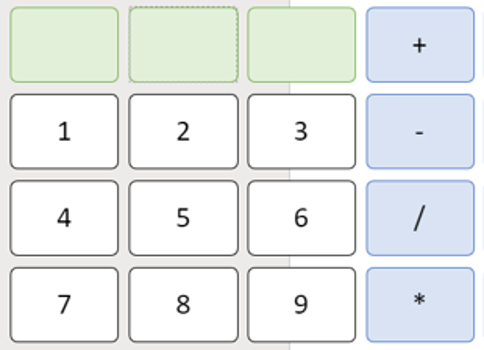
\includegraphics[scale=1]{img/beispiellayout-zum-speichern}
	\caption[Beispiellayout zum Speichern]{Beispiellayout zum Speichern\footnotemark}
\end{figure}

Die Kacheln sind in einem vier-mal-vier Format angelegt. Sie bestehen aus drei Stack-Kacheln, neun Operanden-Kacheln mit einzelnen Zahlen und vier Operatoren-Kacheln. Diese sind repräsentativ für dieses Beispiel, da der Speicherprozess für alle Inhalte einer Art gleich gehandhabt wird.

Nachfolgend ist die CSV-Repräsentation des obigen Layouts abgebildet. 

\begin{figure}[h]
	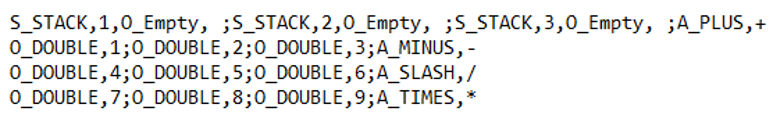
\includegraphics[scale=1]{img/csv-repraesentation-layout}
	\caption[CSV-Repräsentation des Beispiellayouts]{CSV-Repräsentation des Beispiellayouts\footnotemark}
\end{figure}

Entsprechend den CSV-Konventionen beschreibt ein Line Break („\\n“) das Ende einer Reihe des Layouts. Ein Semikolon („;“) beschreibt das Ende einer Spalte. Innerhalb einer einzelnen Zelle werden die Informationen über eine Kachel durch ein Tupel gehalten. Innerhalb des Tupels werden die einzelnen Werte durch ein Komma („,“) getrennt.

In der Regel werden pro Kachel zwei Informationen gespeichert: Die Art der Kachel und der Inhalt oder anzuzeigende Text. So beschreibt das Tupel „O\_DOUBLE,1“ eine Kachel vom Typ ODouble mit dem Inhalt „1“. Lediglich bei Stack- und HistoryStack-Kacheln muss ein Tupel mit vier Inhalten gespeichert werden. Der erst Wert beschreibt auch dort die Art der Kachel. Im zweiten Wert wird der Rang des Stacks, also welche Nummer es im Stack hat, gespeichert. Anschließend wird der enthaltene Operand gespeichert. 

\subsubsection{Klasse: TileLayoutManager}
Das Speichern und Laden von CSV Dateien wird durch diese Klasse implementiert.

\textit{loadLayout}: Laden eines Standardlayouts oder verweis auf den internen Speicher \\
\textit{saveLayout}: Speichert eine CSV in dem internen Speicher \\
\textit{wirteLayout}: Speichert eine CSV in dem internen Speicher \\
\textit{readLayout}: Liest eine CSV aus dem internen Speicher ein \\
\textit{getSavedLayouts}: Gibt eine Liste der gespeicherten Layouts und Standardlayouts (Für Presenter) \\
\textit{clearLayouts}: Löscht alle gespeicherten Layouts (Für Presenter)

\subsubsection{Klasse: TileLayoutFactory}
Die Umformatierung einer CSV Eingabe in ein TileLayout wird in dieser Klasse implementiert.

\textit{createLayout()}: orchestriert das einlesen der CSV Datei und der Erstellung des TileLayouts. \\
\textit{loadLayout()}: Erstellen des TileLayouts aus der CSV


\include{chapter/Dokumentation_der_sonstigen_Beiträge_der_Teammitglieder}

%!TEX root = ../Thesis.tex
\section{Fazits aller Teammitglieder}

\subsection{Dennis Gentges}
Ich empfand es als sehr gut, dass das Modul WIP nicht ausschließlich die reine Programmierung einer Anwendung beinhaltete, sondern ebenfalls das Projektmanagement als essenzieller Bestandteil für eine erfolgreiche Implementierung benötigt wurde. Verglichen mit bereits bekannten Projekten aus dem Betrieb finde ich dies realitätsnaher als es in anderen Modulen der Fall ist. Ein Projekt vom Anfang bis zum Ende zusammen mit einem Team durchzuführen hat mir persönlich viele neue Erkenntnisse und Erfahrungen gebracht.

Neben grundlegenden Projektmanagementmethoden wurden während des Projektes allerdings auch andere Fähigkeiten benötigt, welche ich zu Beginn des Projektes noch nicht beherrschte. Dazu gehörte unter anderem die Arbeit mit GitHub. Dabei benötigte ich eine wesentlich höhere Einarbeitungszeit als andere Kollegen da ich hier noch keine Erfahrungen sammeln konnte. Nach dieser Einarbeitungszeit und mit der Unterstützung der erfahreneren Teammitglieder verstand ich jedoch die Grundfunktionen, sodass ich diese Fähigkeiten nun auch in meinem weiteren Arbeits- und Studienleben einsetzen kann. 
Neben GitHub war mir auch das Textverarbeitungsprogramm Latex noch fremd. Da uns hier ebenfalls jegliche Einweisung fehlte, benötigte ich hierbei wieder eine längere Einarbeitungsphase.

In unserem Projektteam gab es einige sehr gute und geübte Programmierer und ich empfand es als eine große Herausforderung mit dieser Leistung mithalten zu können. Da ich zuvor keine größeren Erfahrungen im Programmieren gesammelt habe und dies auf der Arbeit auch nur begrenzt tun muss, benötigte ich einen wesentlich höheren Zeitaufwand um mich in umgebende Klassen und Methoden einzuarbeiten. Da meine eigentliche zugewiesene Hauptaufgabe in der Projektsteuerung lag, konzentrierte ich mich nun zunächst darauf. Unter der Betrachtung der Meilensteine wurden diese alle fristgerecht erfüllt bzw. eingehalten und wir kamen dem Projektziel Schritt für Schritt näher.

Zusätzlich habe ich den Zeitaufwand für die Fertigstellung der Ausarbeitung unterschätzt. Insbesondere im Zeitraum zwischen November und Februar fielen einige Prüfungsleistungen in der FHDW, aber auch der Abschluss unserer Ausbildung zum Fachinformatiker an. Dies war für alle Teammitglieder eine ziemlich große, zusätzliche Belastung. Am Ende hat es aber dennoch funktioniert.

\clearpage

\subsection{Tom Bockhorn}
Das Projekt zur Erstellung eines Taschenrechners in polnischer Notation sehe ich bereits vor der Abgabe als erfolgreich an. Technisch gesehen sind wir den funktionalen Anforderungen nachgekommen, konnten das Projekt innerhalb des zeitlichen Rahmens zu einem akzeptablen Stand bringen und haben kreative Lösungen für die offenen Fragen der Aufgabenstellung gefunden. Im Laufe des Projektes bekam ich die Gelegenheit mir auf eigene Faust, aber auch in Kommunikation mit meinem Team, neue, spannende Konzepte der Projektdurchführung und Programmierung anzueignen. Auch das zuvor angebaute Wissen aus dem Studium konnte ich einigermaßen in das Projekt mit einbringen, sodass diese Inhalte zusätzlich vertieft wurden. Allein die Größe des Teams bestärkte die Relevanz von Organisation und Kommunikation untereinander. Ich finde die Aufteilung in ein Frontend und Backend Team hat sehr gut funktioniert und selbst zu kritischen Zeitpunkten konnten wir auf Verstärkung durch die anderen zählen.

Für mich persönlich war die Einarbeitung in die Programmierung nur ein geringes Problem, da ich bereits viel Erfahrung mit Java und ein wenig Erfahrung mit Android gewinnen durfte. Dafür stellte sich die Umsetzung der Ausarbeitung in Latex als größere Herausforderung heraus. Dort möchte ich aber unser Team loben, denn es hat sich immer jemand gefunden der Zeit und Motivation hatte sich in uns unbekannte Themen einzuarbeiten!

\clearpage

\subsection{Hendrik Falk}
Aus meiner Sicht war die Projektdurchführung erfolgreich. Die Anforderungen vom Auftraggeber konnten erfolgreich und fristgerecht umgesetzt werden. Dazu zählt neben der Applikation selbst, auch die Dokumentation. 

Meine dispositiven Aufgaben stellten eine sehr neue Herausforderung für mich dar und es bereitete mir Freude daran zu Arbeiten. Sowohl der Umgang mit Android Studio, als auch mich Latex war mir neu und stellte deshalb eine große Herausforderung dar, welche ich aber im für das Projekt benötigten Rahmen bewältigen konnte. Nicht zuletzt dadurch, dass gute Vorarbeit geleistet wurde und How-Tos erstellt wurden, die den Einstieg erleichterten. Die größte Herausforderung war die Überlappung des Projektes mit diversen Prüfungsleistungen im Studium, sowie den Abschlussprüfung unserer Ausbildung als Fachinformatiker. Letzteres fiel genau in die Zeit vor dem angegebenen Projektabschluss und nahm viele unserer Ressourcen in Anspruch.

Dazu kam noch, dass das Team auf verschiedene Standorte verteilt war. Darunter auch Wuppertal und Monheim. Außerdem hatten wir einen Kollegen, der von einer anderen Firma beschäftigt war. Dadurch musste viel Kommunikation digital stattfinden, was Selbige erschwerte. 

Die Kommunikation innerhalb des Teams habe ich als sehr positiv wahrgenommen und verlief stets problemorientiert. Auch in schwierigen Situationen konnten wir Zusammenhalt beweisen und weiterkommen. Somit konnte das Projekt erfolgreich abgeschlossen werden, wobei ich viele neue Erfahrungen machte, die mir auch im späteren Berufsleben weiterhelfen werden.

\clearpage

\subsection{Getuart Istogu}
Rückblickend konnte ich aus dem Projekt viele neue Erkenntnisse gewinnen, zumal es mein erstes Projekt mit mehreren Beteiligten war. Dadurch wurde mir bewusst, wie wichtig eine gute Aufgabenverteilung und Absprache innerhalb eines Teams ist. Außerdem wurde mir durch das Projekt bewusst, wie wichtig eine gute Dokumentation ist, da ich für meine Entwicklung nachvollziehen musste, was das Frontend gemacht hat, um bei der Implementierung der Menüführung auszuhelfen. Zudem war die Dokumentation ein wichtiger Bestandteil bei der Wiederaufnahme der Programmierung nach einer längeren Pause, bedingt durch weitere Prüfungsleistungen im Studium und der Endphase des IHK-Abschlusses als Fachinformatiker.

Generell verlief das Projekt aus meiner Sicht gut. Wir konnten die Anforderungen fristgerecht erfüllen. Dabei konnte ich vor allem den Umgang von GitHub und Latex erlernen. Ich lernte Latex Wert zu schätzen, dadurch dass die Ausarbeitung ohne viel Mehraufwand sehr einheitlich aussah. Zuerst viel mir der Umgang damit jedoch schwer. Die Einarbeitung in GitHub war für mich auch sehr aufwändig, jedoch konnte ich von dem Wissen der anderen Teammitglieder profitieren. 

Des Weiteren hatte ich bereits eine mobile App für iOS entwickelt. Dafür habe ich aber die Programmiersprache C\# und das dazugehörige Framework Xamarin verwendet. Was mir dabei aufgefallen ist, dass besonders im Frontendbereich sehr viele Ähnlichkeiten gab und das Einarbeiten vereinfacht hat. Weitere auffallende Gemeinsamkeiten beziehungsweise Unterschiede sind mir nicht aufgefallen. 

Für das Backend habe ich zunächst Unittests in einem Projekt implementiert und war erstaunt, wie einfach sie zu implementieren sind. Besonders der Aspekt, dass leicht nachvollzogen werden kann, ob die Methoden wie erwartet funktionieren. Dies kann dann losgelöst vom Frontend überprüft werden, dass auch wichtig für das Projekt waren.
Ich hatte am Anfang meine Bedenken gehabt, ob wir die Anforderungen an den Taschenrechner umsetzen konnten, aber diese Bedenken lösten sich im Laufe des Projektes auf.

\clearpage

\subsection{Jannis Keienburg}
Für mich war dies das erste Programmierprojekt mit mehreren Beteiligten. Ebenfalls war es die erste große Java- bzw. Android-Applikation, an der ich entwickelt habe. Die größte Herausforderung aus meiner Sicht war die Kommunikation innerhalb des Teams. Es war teilweise schwierig zu erfahren, wer gerade bei welchem Thema wie weit war. Innerhalb meines Aufgabenbereiches war die größte Herausforderung für mich die Programmierung der Klasse zur Berechnung der Hoch- und Tiefpunkte. Grund dafür war zum einen die Abhängigkeit zu der Klasse Zeros, aber auch viele kleine Fehler, die erst mit zeilenweisem Debugging gefunden und gelöst werden konnten. Das Lesen der Codebeiträge der anderen Beteiligten war anfangs etwas schwierig, im Laufe des Projektverlaufes wurde dies allerdings immer einfacher, auch weil die Klassen gut kommentiert wurden. Alles in allem ein lehrreiches und für den späteren Berufsweg wegweisendes Projekt.

\clearpage

\subsection{Tim Jonas Meinerzhagen}
Ich werde nachfolgend ein kurzes Fazit zur erstellten App, unserer Arbeit im Team und meinem Beitrag zum Projekt geben.

Die von uns erstellte App konnte allen gestellten Anforderungen entsprechend umgesetzt werden. Es wurde eine breite Spanne an Funktionalitäten implementiert, welche verschiedenste Bereiche abdeckt. Alle Kacheln können dynamisch angepasst werden. In der Ausführung ist die App sehr stabil und es treten keine größeren Bugs auf, die einen Crash herbeiführen könnten. An einigen Stellen wären noch Anpassungen hilfreich gewesen, um eine bessere User Experience herbeizuführen, dies wurde allerdings auf Grund der begrenzten Zeit als akzeptabel angesehen. Insgesamt bin ich sehr zufrieden mit dem letztlichen Stand der App.

Das Projekt in unserem Team „Das Proletariat“ ist sehr harmonisch verlaufen. Alle Teammitglieder konnten ihren Beitrag zum Projekterfolg leisten. Es war das erste Mal, dass wir ein Softwareprojekt unter Beteiligung von acht Entwicklern durchführen mussten. Dies erforderte eine umfassende Organisation, welche Dennis und Hendrik herausragend geleistet haben. Dadurch, dass wir auch bereits seit mehreren Jahren zusammen studieren, war die Zusammenarbeit sehr harmonisch, was auch bei Meinungsverschiedenheiten beibehalten werden konnte.  Die Projektdurchführung im Team habe ich als sehr produktiv war genommen.

Als Teil des Architektur-Teams, welches eine Schnittstellenfunktion darstellte, war ich an einem breiten Spektrum von Aufgaben beteiligt. Dies hat dazu geführt, dass ich einen umfassenden Einblick in die verschiedenen Strukturen des Projektes erhalten konnte. 
Letztlich komme ich noch zu meinem eigenen Beitrag zum Projekt. Dadurch, dass ich bereits Vorerfahrung mit der Programmierung von Android Apps hatte, konnte ich während der Planung und der Umsetzung als Experte in diesem Bereich fungieren. So konnte ich mich schneller in die verschiedenen Bereiche der App einarbeiten und helfen, wenn notwendig. 

\clearpage

\subsection{Khang Pham}
Insgesamt kann die Durchführung des Projektes als erfolgreich angesehen werden. Die Anforderungen wie sie in der Aufgabenstellung beschrieben sind und wie sie mit dem Auftraggeber besprochen wurden, konnten allesamt vollständig bzw. in Ansätzen umgesetzt werden (Das heißt es konnten alle Operatoren umgesetzt werden. Der Operand ‘‘Multiplikation’‘ beispielsweise, ist allerdings für den Operator ‘‘Matrizen’‘ nicht funktional). Da die Taschenrechner-Applikation jedoch nicht für den tatsächlichen Einsatz mit echten Anwendern entwickelt wurde, war eine hundertprozentige Umsetzung aller Funktionen, auch in Anbetracht des zeitlichen Rahmens kein Ziel des Projektes. Vielmehr konnte eine Applikation entwickelt werden, welche zum einen alle Grundanforderungen eines Taschenrechners mit UPN umsetzt, und zum anderen die entwickelten Konzepte für Kachellayout und Usability widerspiegelt. Die Recherche, die das Team außerhalb der Vorlesungen durchführen musste um die Entwicklung einer App in Android zu erlernen, das Koordinieren zwischen den einzelnen Teammitgliedern für die Durchführung und Zeitplanung des Projektes, sowie die Verteilung der Arbeitspakete innerhalb des Projektes bildeten für die Projektteilnehmer eine neue, wertvolle Erfahrung.
Insbesondere für mich war die Arbeit an einem Softwareprojekt als einer von vielen Entwicklern eine neuartige und sehr interessante Erfahrung. Auch die Arbeit mit GIT empfand ich als sehr interessant, da ich auf der Arbeit noch nicht damit arbeiten konnte. Der benötigte Verwaltungsoverhead für ein solches Projekt mit einer großen Anzahl an beteiligten Entwicklern stellte sich als deutlich größer heraus, als ich ursprünglich annahm. Insgesamt sammelte ich während des Projektes viele neue und wertvolle Erfahrungen für mich, die auch für meine zukünftige Arbeit als IT-Consultant relevant werden könnten. 

\clearpage

\subsection{Tim Schwenke}

Die Entwicklung des RPN-Tile-Calculators hat viele Inhalte aus den Modulen des Studiums aufgegriffen. Jedoch liegt der grö\ss te Erfahrungsgewinn für mich persönlich in der engen Zusammenarbeit mit dem gesamten Projektteam.

So habe ich schon bei vielen Projekten die Möglichkeit gehabt mein Wissen in Bezug auf Entwurf und Entwicklung von Software anzuwenden und zu erweitern. Besonders hervorzuheben sind hier berufliche Projekt im Rahmen meines Dualen Studiums. Jedoch sind viele der Projekte relativ isoliert gewesen. Meist war ich gesamtverantwortlich für das Projekt und musste auf kein Projektteam Rücksicht nehmen. Im Gegensatz dazu hat die Entwicklung des Taschenrechners produktive Zusammenarbeit mit allen Mitgliedern erfordert. Ich musste nicht nur meine eigenen Aufgabenpakete pünktlich und korrekt umsetzen, sondern auch Vertrauen in die Arbeit meiner Teammitglieder haben. Dieses Vertrauen innerhalb des Teams hat das Projekt zum Erfolg geführt.

Aus technischer Sicht habe ich wiederholt gesehen, wie wichtig wohldefinierte Schnittstellen sind, um verteilt und parallel an einem Projekt arbeiten zu können. Ist nicht klar, wie genau eine Schnittstelle überhaupt aussehen soll oder das Konzept bestimmter Bestandteile der Software überhaupt ist (z.B. Kalkulationsorchestrierung), kann man nicht effektiv arbeiten. Dafür ist ein vollständiger kommunizierter Plan notwendig, dem alle Mitglieder zustimmen. Deswegen ist es nicht möglich ohne Austausch ''vor sich hin zu programmieren'', wie es bei einem Ein-Mann-Projekt der Fall wäre.

Zusammenfassend lässt sich sagen, dass das Projekt fordernd aber auch gleichzeitig lohnenswert gewesen ist. Ich bin zuversichtlich die dazugewonnenen Erfahrungen zukünftig gewinnbringend einsetzen zu können.


%%%%%%%%%%%%%%%%%%%%%%%%%%%%%%%%%%%%%%%%%%%%%%%%%%%%%%%%%%%%%%%%%%%%%%%
%% Anhang
%%%%%%%%%%%%%%%%%%%%%%%%%%%%%%%%%%%%%%%%%%%%%%%%%%%%%%%%%%%%%%%%%%%%%%%

%!TEX root = ../Thesis.tex

\section{Anhang - Quelltext}

\subsection{Model}

\subsubsection{Calculation}

\begin{lstlisting}[caption=Action (Schwenke),label=list:Action,language=Java]
package de.fhdw.wip.rpntilecalculator.model.calculation;

import de.fhdw.wip.rpntilecalculator.model.operands.Operand;

import org.jetbrains.annotations.Contract;
import org.jetbrains.annotations.NotNull;

import java.lang.reflect.InvocationTargetException;
import java.util.List;

/**
 * Summary: The framework for defining Actions. Actions are able to work with operands from the stack or executor functions.
 * Author:  Tim Schwenke
 * Date:    2020/01/04
 */
public abstract class Action {

    /**
     * Must be set by inheriting classes of {@link Action} for reflection to work.
     */
    protected Action scopedAction;

    /**
     * Must be overridden in case the required number of operands is a fixed amount.
     */
    protected int[] requiredNumOfOperands = new int[]{-1};

    /**
     * Leverages reflection for matching given arguments to a calculation method.
     *
     * @param operands List of operands.
     * @return Always a valid Operand.
     * @throws CalculationException In case the result cannot be computed.
     */
    @Contract(pure = true)
    public @NotNull Operand with(@NotNull List<Operand> operands) throws CalculationException {
        Operand[] target = new Operand[operands.size()];
        for (int i = 0; i < target.length; i++) {
            target[i] = operands.get(i);
        }
        return with(target);
    }

	/**
     * Leverages reflection for matching given arguments to a calculation method.
     *
     * @param operands List of operands.
     * @return Always a valid Operand.
     * @throws CalculationException In case the result cannot be computed.
     */
    @Contract(pure = true) public @NotNull Operand with(@NotNull Operand... operands) throws CalculationException {
        Class[] operandClasses = new Class[operands.length];
        Operand resultOperand;

        for (int i = 0; i < operands.length; i++)
            operandClasses[i] = operands[i].getClass();

        try {
            resultOperand = (Operand) scopedAction.getClass()
                    .getDeclaredMethod(
                            "on",
                            operandClasses
                    ).invoke(
                            scopedAction,
                            (Object[]) operands
                    );
        } catch (RuntimeException | NoSuchMethodException | IllegalAccessException | InvocationTargetException e) {
            throw new CalculationException(e.getMessage());
        }

        if (resultOperand != null) return resultOperand;
        else throw new CalculationException();
    }

    /**
     * @return Number of required operands for the concrete {@link Action}. If {@code -1}
     * the number of operands required is variable.
     */
    public int[] getRequiredNumOfOperands() {
        return requiredNumOfOperands;
    }

}
\end{lstlisting}    

\begin{lstlisting}[caption=ArcCosinus (Keienburg),label=list:ArcCosinus,language=Java]
package de.fhdw.wip.rpntilecalculator.model.calculation;

import org.jetbrains.annotations.Contract;
import org.jetbrains.annotations.NotNull;

import de.fhdw.wip.rpntilecalculator.model.operands.ODouble;
import de.fhdw.wip.rpntilecalculator.model.operands.Operand;

/*
 * Summary: Defines the arc Cosinus action.
 * Author:  Jannis Luca Keienburg
 * Date:    2020/01/04
 */

public class ArcCosinus extends Action {

    @NotNull
    private static final ArcCosinus ARC_COSINUS = new ArcCosinus();

    /*
     * Singleton for COSINUS
     * @return singleton object
     */
    @Contract(pure = true) @NotNull public static ArcCosinus getInstance() { return ARC_COSINUS; }
    private ArcCosinus() {
        requiredNumOfOperands = new int[]{1};
    }

    @NotNull @Override
    public Operand with(@NotNull Operand... operands) throws CalculationException {
        scopedAction = this;
        return super.with(operands);
    }

    /**
     * Calculates the arc cosinus with a given angle.
     *
     * @param angle Representing the angle.
     * @return Result
     */
    @Contract(pure = true) @NotNull ODouble on(@NotNull ODouble angle) {
        return new ODouble(Math.acos(Math.toRadians((angle.getDouble()))));
    }
}
\end{lstlisting}    

\begin{lstlisting}[caption=ArcSinus (Keienburg),label=list:ArcSinus,language=Java]
package de.fhdw.wip.rpntilecalculator.model.calculation;

import org.jetbrains.annotations.Contract;
import org.jetbrains.annotations.NotNull;

import de.fhdw.wip.rpntilecalculator.model.operands.ODouble;
import de.fhdw.wip.rpntilecalculator.model.operands.Operand;

/*
 * Summary: Defines the arc Sinus action.
 * Author:  Jannis Luca Keienburg
 * Date:    2020/01/04
 */

public class ArcSinus extends Action {

    @NotNull
    private static final ArcSinus ARC_SINUS = new ArcSinus();

    /*
     * Singleton for SINUS
     * @return singleton object
     */
    @Contract(pure = true) @NotNull public static ArcSinus getInstance() { return ARC_SINUS; }
    private ArcSinus() {
        requiredNumOfOperands = new int[]{1};
    }

    @NotNull @Override
    public Operand with(@NotNull Operand... operands) throws CalculationException {
        scopedAction = this;
        return super.with(operands);
    }

    // Calculates the arc sinus with a given angle.
    @Contract(pure = true) @NotNull ODouble on(@NotNull ODouble angle) {
        return new ODouble(Math.asin(Math.toRadians((angle.getDouble()))));
    }
}
\end{lstlisting}    

\begin{lstlisting}[caption=ArcTangens (Keienburg),label=list:ArcTangens,language=Java]
package de.fhdw.wip.rpntilecalculator.model.calculation;

import org.jetbrains.annotations.Contract;
import org.jetbrains.annotations.NotNull;

import de.fhdw.wip.rpntilecalculator.model.operands.ODouble;
import de.fhdw.wip.rpntilecalculator.model.operands.Operand;

/*
 * Summary: Defines the arc Tangens action.
 * Author:  Jannis Luca Keienburg
 * Date:    2020/01/04
 */

public class ArcTangens  extends Action {

    @NotNull
    private static final ArcTangens ARC_TANGENS = new ArcTangens();

    /*
     * Singleton for SINUS
     * @return singleton object
     */
    @Contract(pure = true) @NotNull public static ArcTangens getInstance() { return ARC_TANGENS; }
    private ArcTangens() {
        requiredNumOfOperands = new int[]{1};
    }

    @NotNull @Override
    public Operand with(@NotNull Operand... operands) throws CalculationException {
        scopedAction = this;
        return super.with(operands);
    }

    // Calculates the tangens with a given angle.
    @Contract(pure = true) @NotNull ODouble on(@NotNull ODouble angle) {
        return new ODouble(Math.atan(Math.toRadians((angle.getDouble()))));
    }
}
\end{lstlisting}    

\begin{lstlisting}[caption=CalculationException (Schwenke),label=list:CalculationException,language=Java]
package de.fhdw.wip.rpntilecalculator.model.calculation;

/**
 * Summary: Main Exception for a failed Calculation
 * Author:  Tim Schwenke
 * Date:    2020/01/04
 */
public class CalculationException extends Exception {

    /**
     * Create a new Exception
     * @param msg Error Message
     */
    public CalculationException(String msg) {
        super(msg);
    }

    /**
     * Create a new standard Exception
     */
    public CalculationException() {
        this("Not supported");
    }
}
\end{lstlisting}    

\begin{lstlisting}[caption=Cosinus (Keienburg),label=list:Cosinus,language=Java]
package de.fhdw.wip.rpntilecalculator.model.calculation;

import de.fhdw.wip.rpntilecalculator.model.operands.ODouble;
import de.fhdw.wip.rpntilecalculator.model.operands.Operand;

import org.jetbrains.annotations.Contract;
import org.jetbrains.annotations.NotNull;

/*
 * Summary: Defines the Cosinus action.
 * Author:  Jannis Luca Keienburg
 * Date:    2020/01/04
 */
@SuppressWarnings({"unused"})
public class Cosinus extends Action {

    @NotNull
    private static final Cosinus COSINUS = new Cosinus();

    /*
     * Singleton for COSINUS
     * @return singleton object
     */
    @Contract(pure = true) @NotNull public static Cosinus getInstance() { return COSINUS; }
    private Cosinus() {
        requiredNumOfOperands = new int[]{1, 2};
    }

    @NotNull @Override
    public Operand with(@NotNull Operand... operands) throws CalculationException {
        scopedAction = this;
        return super.with(operands);
    }

    // Calculates the cosinus with a given angle.
    @Contract(pure = true) @NotNull ODouble on(@NotNull ODouble angle) {
        return new ODouble(Math.cos(Math.toRadians((angle.getDouble()))));
    }
}
\end{lstlisting}    

\begin{lstlisting}[caption=Derivation (Keienburg),label=list:Derivation,language=Java]
package de.fhdw.wip.rpntilecalculator.model.calculation;

import org.apache.commons.math3.analysis.polynomials.PolynomialFunction;

import org.jetbrains.annotations.Contract;
import org.jetbrains.annotations.NotNull;

import de.fhdw.wip.rpntilecalculator.model.operands.OPolynom;
import de.fhdw.wip.rpntilecalculator.model.operands.Operand;

/*
 * Summary: A Class that can calculate the derivate of a function
 * Author:  Jannis Luca Keienburg
 * Date:    2020/01/14
 */

public class Derivation extends Action {

    @NotNull private static final Derivation DERIVATION = new Derivation();

    @Contract(pure = true) @NotNull public static Derivation getInstance() { return DERIVATION; }
    private Derivation() {
        requiredNumOfOperands = new int[]{1};
    }

    @NotNull @Override
    public Operand with(@NotNull Operand... operands) throws CalculationException {
        scopedAction = this;
        return super.with(operands);
    }

    @Contract(pure = true) @NotNull OPolynom on(@NotNull OPolynom oPolynom) {
        return derivate(oPolynom);
    }

    // Structure: via the method getCoefficients()
    // coefficients[n] * x^n + ... + coefficients[1] * x + coefficients[0]

    // Sets the Function into the following formatition:
    // [n]* x^10 + [n-1] *x^9 + ... + [1] * x + [0]
    private double[] getFunctionAsDouble(@NotNull OPolynom oPolynom) {
        return oPolynom.getPolynom().getCoefficients();
    }

    // Calculates the derivation
    // returns it as an OPolynom
    public OPolynom derivate(OPolynom oPolynom)
    {
        double[] function = getFunctionAsDouble(oPolynom);
        double[] derivation = new double[function.length - 1];

        for(int i = function.length - 1; i > 0; i--)
        {
            derivation[i-1] = function[i] * i;
        }
        return new OPolynom(new PolynomialFunction(derivation));
    }
}
\end{lstlisting}    

\begin{lstlisting}[caption=HighAndLowPoints (Keienburg),label=list:HighAndLowPoints,language=Java]
package de.fhdw.wip.rpntilecalculator.model.calculation;

import org.apache.commons.math3.analysis.polynomials.PolynomialFunction;

import org.intellij.lang.annotations.JdkConstants;
import org.jetbrains.annotations.Contract;
import org.jetbrains.annotations.NotNull;

import de.fhdw.wip.rpntilecalculator.model.operands.OPolynom;
import de.fhdw.wip.rpntilecalculator.model.operands.OTuple;
import de.fhdw.wip.rpntilecalculator.model.operands.Operand;

/*
 * Summary: A Class that can calculate the high and the low points of a function( up to third grade)
 * Author:  Jannis Luca Keienburg
 * Date:    2020/01/16, updated on 2020/01/17
 */

public class HighAndLowPoints extends Action {

    @NotNull private static final HighAndLowPoints HIGH_AND_LOW_POINTS = new HighAndLowPoints();
    @NotNull private static final Derivation DERIVATION = Derivation.getInstance();
    @NotNull private static final Zeros ZEROS = Zeros.getInstance();

    @Contract(pure = true) @NotNull public static HighAndLowPoints getInstance() { return HIGH_AND_LOW_POINTS; }
    private HighAndLowPoints() {
        requiredNumOfOperands = new int[]{1};
    }

    @NotNull @Override
    public Operand with(@NotNull Operand... operands) throws CalculationException {
        scopedAction = this;
        return super.with(operands);
    }

    @Contract(pure = true) @NotNull OTuple on(@NotNull OPolynom oPolynom) {
        return new OTuple(getHighAndLowPoints(oPolynom));
    }

    // Begin. Returns an double array with the following structure
    public double [] getHighAndLowPoints(OPolynom oPolynom)
    {
        double [] result = calculateHighAndLowPoints(oPolynom);
        return result;
    }

    // Sets the Function into the following formatition:
    // [n]* x^10 + [n-1] *x^9 + ... + [1] * x + [0]
    private double[] getFunctionAsDouble(OPolynom oPolynom) {
        return oPolynom.getPolynom().getCoefficients();
    }

    // Calculates the values of the extreme points of a given function.
    // Returns the values as an double array, an uneyual number position stands for the x value,
    // the number at the next position for the y value
    private double[] calculateHighAndLowPoints(OPolynom oPolynom)
    {
        // Calculates the derivation of the funcion.
        OPolynom derivation = DERIVATION.derivate(oPolynom);
        // Calculates the zeros of the function's derivation.
        double [] zeros = ZEROS.calculateZeros(derivation);
        // Gets the funcion as an double array for the calculation.
        double [] functionAsDouble = getFunctionAsDouble(oPolynom);

        // Calculates the y values of the zeros.
        double [] valuesXY = new double[] {};
        int position = -1;
        for(int counter = 0; counter < zeros.length; counter++)
        {
            double currentZero = zeros[counter];
            double yValue = 0;
            for(int counter2 = 0; counter < functionAsDouble.length; counter2++)
            {
                yValue += functionAsDouble[counter] * Math.pow(currentZero,(functionAsDouble.length - counter2 - 1));
            }
            position++;
            valuesXY[position] = currentZero;
            position++;
            valuesXY[position] = yValue;
        }
        return valuesXY;
    }
}
\end{lstlisting}    

\begin{lstlisting}[caption=Integral (Istogu),label=list:Integral,language=Java]
package de.fhdw.wip.rpntilecalculator.model.calculation;

import org.apache.commons.math3.analysis.UnivariateFunction;
import org.apache.commons.math3.analysis.integration.SimpsonIntegrator;
import org.apache.commons.math3.analysis.polynomials.PolynomialFunction;
import org.jetbrains.annotations.Contract;
import org.jetbrains.annotations.NotNull;

import de.fhdw.wip.rpntilecalculator.model.operands.ODouble;
import de.fhdw.wip.rpntilecalculator.model.operands.OPolynom;
import de.fhdw.wip.rpntilecalculator.model.operands.Operand;

/*
 * Summary: Calculate the antiderivative and integral
 * Author:  Getuart Istogu
 * Date:    2020/01/27
 */

public class Integral extends Action {

    @NotNull private static final Integral INTEGRAL = new Integral();

    @Contract(pure = true) @NotNull public static Integral getInstance() { return INTEGRAL; }
    private Integral() {requiredNumOfOperands = new int[] {3};}

    @NotNull @Override
    public Operand with(@NotNull Operand... operands) throws CalculationException {
        scopedAction = this;
        return super.with(operands);
    }

    @Contract(pure = true) @NotNull ODouble on(@NotNull OPolynom oPolynom, @NotNull ODouble lowerBound, @NotNull ODouble upperBound) {
        return calculateIntegralSimpsons(oPolynom, lowerBound.getDouble(), upperBound.getDouble());
    }
    
    /**
     * Calculates the integral for the specified limit range
     * @param oPolynom Normal PolynomialFunction, not its antiderivative
     * @param lowerBound Lower limit
     * @param upperBound Upper limit
     * @return
     */
    @NotNull
    public ODouble calculateIntegralSimpsons(OPolynom oPolynom, double lowerBound, double upperBound)
    {
        SimpsonIntegrator simpsonIntegrator = new SimpsonIntegrator();
        UnivariateFunction uF = (UnivariateFunction) oPolynom.getPolynom();
        return new ODouble(simpsonIntegrator.integrate(10000, uF, lowerBound, upperBound));
    }

    /**
     * Calculates the antiderivative of the passed function
     * @param oPolynom Examined function
     * @return Its antiderivative
     */
    public OPolynom getAntiderivative(OPolynom oPolynom)
    {
        PolynomialFunction polynomialFunction = oPolynom.getPolynom();

        // 3x^2 -2x +5 == 3rd degree, but 4 coefficients
        // Therefore number of coefficient antiderivative = degree + 2
        int degreeForAntiderivative = polynomialFunction.degree() + 2;

        double[] functionCoefficents = polynomialFunction.getCoefficients();

        double[] antiderivativeCoefficents = new double[degreeForAntiderivative];

        // This value can be of any size. It is referred as "C" in the literature.
        antiderivativeCoefficents[0] = 0;
        for(int i = 1; i < degreeForAntiderivative; i++)
        {
            antiderivativeCoefficents[i] = functionCoefficents[i-1]/((double) i);
        }

        return new OPolynom(new PolynomialFunction(antiderivativeCoefficents));
    }
}
\end{lstlisting}    

\begin{lstlisting}[caption=Limes (Istogu),label=list:Limes,language=Java]
package de.fhdw.wip.rpntilecalculator.model.calculation;

import org.apache.commons.math3.analysis.polynomials.PolynomialFunction;

import org.jetbrains.annotations.Contract;
import org.jetbrains.annotations.NotNull;

import de.fhdw.wip.rpntilecalculator.model.operands.ODouble;
import de.fhdw.wip.rpntilecalculator.model.operands.OPolynom;
import de.fhdw.wip.rpntilecalculator.model.operands.Operand;


/*
 * Summary: Determine limit
 * Author:  Getuart Istogu
 * Date:    2020/01/04
 */
public class Limes extends Action {

    @NotNull private static final Limes LIMES = new Limes();

    @Contract(pure = true) @NotNull public static Limes getInstance() { return LIMES; }
    private Limes() { requiredNumOfOperands = new int[] {2};}

    @NotNull @Override
    public Operand with(@NotNull Operand... operands) throws CalculationException {
        scopedAction = this;
        return super.with(operands);
    }

    @Contract(pure = true) @NotNull ODouble on (@NotNull OPolynom oPolynom, @NotNull ODouble approach) {
        return limit(oPolynom, approach.getDouble());
    }

    /**
     * Calculates the limit of a function at one point
     * @param oPolynom Examined function
     * @param approach Limit point
     * @return Limit value at the defined point
     */
    public ODouble limit(OPolynom oPolynom, double approach) {
        PolynomialFunction polynomialFunction = oPolynom.getPolynom();
        double below = limitFromBelow(polynomialFunction, approach);
        double above = limitFromAbove(polynomialFunction, approach);
        if(below == above)
            return new ODouble(below);
        else
            return new ODouble(Double.NaN);
    }

    /**
     * Calculates the limit of a function at one point from below
     * @param polynomialFunction Examined function
     * @param approach Limit point
     * @return Limit value from below at the defined point
     */
    private double limitFromBelow(PolynomialFunction polynomialFunction, double approach) {

        for (double d = approach - 10; d <= approach; d = approach
                - ((approach - d) / 10)) {
            if (polynomialFunction.value(d) == Double.POSITIVE_INFINITY) {
                return Double.POSITIVE_INFINITY;
            } else if (polynomialFunction.value(d) == Double.NEGATIVE_INFINITY) {
                return Double.NEGATIVE_INFINITY;
            } else if (Double.isNaN(polynomialFunction.value(d))) {
                return polynomialFunction.value(approach + ((approach - d) * 10));
            } else {
                if (d == approach) {
                    return polynomialFunction.value(d);
                } else if (approach - d < 0.00000000001) {
                    d = approach;
                }
            }
        }
        return Double.NaN;
    }

    /**
     * Calculates the limit of a function at one point from above
     * @param polynomialFunction Examined function
     * @param approach Limit point
     * @return Limit value from above at the defined point
     */
    private double limitFromAbove(PolynomialFunction polynomialFunction, double approach) {

        for (double d = approach + 10; d >= approach; d = approach
                - ((approach - d) / 10)) {
            if (polynomialFunction.value(d) == Double.POSITIVE_INFINITY) {
                return Double.POSITIVE_INFINITY;
            } else if (polynomialFunction.value(d) == Double.NEGATIVE_INFINITY) {
                return Double.NEGATIVE_INFINITY;
            } else if (Double.isNaN(polynomialFunction.value(d))) {
                return polynomialFunction.value(approach + ((approach - d) * 10));
            } else {
                if (d == approach) {
                    return polynomialFunction.value(d);
                } else if (d - approach < 0.00000000001) {
                    d = approach;
                }
            }
        }
        return Double.NaN;
    }
}
\end{lstlisting}    

\begin{lstlisting}[caption=Logarithm (Keienburg),label=list:Logarithm,language=Java]
package de.fhdw.wip.rpntilecalculator.model.calculation;


import org.jetbrains.annotations.Contract;
import org.jetbrains.annotations.NotNull;

import de.fhdw.wip.rpntilecalculator.model.operands.ODouble;
import de.fhdw.wip.rpntilecalculator.model.operands.Operand;

/*
 * Summary: A Class that can calculate the natural logarithm.
 * Author:  Jannis Luca Keienburg
 * Date:    2020/01/19
 */
public class Logarithm extends Action {

    @NotNull
    private static final Logarithm LOGARITHM = new Logarithm();

    /*
     * Singleton for Logarithm
     * @return singleton object
     */
    @Contract(pure = true) @NotNull public static Logarithm getInstance() { return LOGARITHM; }
    private Logarithm() {
        requiredNumOfOperands = new int[]{1, 2};
    }

    @NotNull @Override
    public Operand with(@NotNull Operand... operands) throws CalculationException {
        scopedAction = this;
        return super.with(operands);
    }

    //Natural Logarithm
    @Contract(pure = true) @NotNull ODouble on(@NotNull ODouble oDouble) {
        if(oDouble.getDouble() <= 0)
            throw new IllegalArgumentException("Value must be higher than Zero.");
        return new ODouble(Math.log(oDouble.getDouble()));
    }

    //Logarithm with specific base
    @Contract(pure = true) @NotNull ODouble on(@NotNull ODouble base, ODouble logartihmOf) {
        if(base.getDouble() <= 0 || logartihmOf.getDouble() <= 0)
            throw new IllegalArgumentException("Value must be higher than Zero.");
        return new ODouble(Math.log(logartihmOf.getDouble()) / Math.log(base.getDouble()));
    }
}
\end{lstlisting}    

\begin{lstlisting}[caption=Logarithm10 (Keienburg),label=list:Logarithm10,language=Java]
package de.fhdw.wip.rpntilecalculator.model.calculation;

import org.jetbrains.annotations.Contract;
import org.jetbrains.annotations.NotNull;
import de.fhdw.wip.rpntilecalculator.model.operands.ODouble;
import de.fhdw.wip.rpntilecalculator.model.operands.Operand;

/*
 * Summary: A Class that can calculate the natural logarithm.
 * Author:  Jannis Luca Keienburg
 * Date:    2020/01/19
 */
public class Logarithm10 extends Action {

    @NotNull
    private static final Logarithm10 LOGARITHM10 = new Logarithm10();

    /*
     * Singleton for Logarithm with the base of 10
     * @return singleton object
     */
    @Contract(pure = true) @NotNull public static Logarithm10 getInstance() { return LOGARITHM10; }
    private Logarithm10() {
        requiredNumOfOperands = new int[]{1};
    }

    @NotNull @Override
    public Operand with(@NotNull Operand... operands) throws CalculationException {
        scopedAction = this;
        return super.with(operands);
    }

    //Logarithm to the base of 10
    @Contract(pure = true) @NotNull ODouble on(@NotNull ODouble oDouble) {
        if(oDouble.getDouble() <= 0)
            throw new IllegalArgumentException("Value must be higher than Zero.");
        return new ODouble(Math.log10(oDouble.getDouble()));
    }
}
\end{lstlisting}  

\begin{lstlisting}[caption=MatrixUtil (Istogu),label=list:MatrixUtil,language=Java]
package de.fhdw.wip.rpntilecalculator.model.calculation;

import org.jetbrains.annotations.Contract;
import org.jetbrains.annotations.NotNull;

import de.fhdw.wip.rpntilecalculator.model.operands.OMatrix;
import de.fhdw.wip.rpntilecalculator.model.operands.OSet;
import de.fhdw.wip.rpntilecalculator.model.operands.OTuple;
import de.fhdw.wip.rpntilecalculator.model.operands.Operand;

/*
 * Summary: Solving systems of linear equations with "LR decomposition with column pivot search"
 * Author:  Getuart Istogu
 * Date:    2020/01/27
 */

public class MatrixUtil extends Action {
    @NotNull
    private static final MatrixUtil MATRIX_UTIL  = new MatrixUtil();

    @Contract(pure = true) @NotNull public static MatrixUtil getInstance() { return MATRIX_UTIL; }
    private MatrixUtil() { requiredNumOfOperands = new int[] {2}; }

    @NotNull @Override
    public Operand with(@NotNull Operand... operands) throws CalculationException {
        scopedAction = this;
        return super.with(operands);
    }

    @Contract(pure = true) @NotNull OTuple on (@NotNull OMatrix A, OTuple b) {
        return solveLinearSystem(A, b.getTuple());
    }
    /**
     * On the condition that A*x = b
     * @param A Matrix
     * @param b Solution vector
     * @return Returns the vector 'x'
     */
    public OTuple solveLinearSystem(OMatrix A, double[] b)
    {
        return new OTuple(solveLGSForX(A.getMatrix().getData(), b));
    }

    /**
     * Determines pivot vector
     * @param A The linear system in double[][]
     * @return
     */
    private int[] pivot(double A[][])
    {
        int n = A.length;
        int[] pivot = new int[n];
        for (int j = 0; j < n-1; j++)
        {
            double max = Math.abs(A[j][j]);
            int imax = j;
            for (int i = j+1; i < n; i++)
                if (Math.abs(A[i][j]) > max)
                {
                    max  = Math.abs(A[i][j]);
                    imax = i;
                }
            double[] h = A[j];
            A[j] = A[imax];
            A[imax] = h;
            pivot[j] = imax;
            for (int i = j+1; i < n; i++)
            {
                double f = -A[i][j]/A[j][j];
                for (int k = j+1; k < n; k++)
                    A[i][k] += f*A[j][k];
                A[i][j] = -f;
            }
        }
        return pivot;
    }

    /**
     * Loest das LGS A*x = b nach x auf
     * @param A The linear system in double[][]
     * @param b Solution vector
     * @return Returns the vector 'x'
     */
    private double[] solveLGSForX(double[][] A, double[] b)
    {
        double[][] B = A.clone();
        double[] x = b.clone();
        int[] pivot = pivot(B);
        int n = B.length;
        for (int i = 0; i < n-1; i++)
        {
            double h = b[pivot[i]];
            b[pivot[i]] = b[i];
            b[i] = h;
        }
        for (int j = 0; j < n; j++)
        {
            x[j] = b[j];
            for (int i = 0; i < j; i++)
                x[j] -= B[j][i]*x[i];
        }
        for (int j = n-1; j >= 0; j--)
        {
            for (int k = j+1; k < n; k++)
                x[j] -= B[j][k]*x[k];
            x[j] /= B[j][j];
        }
        return x;
    }
}
\end{lstlisting}    

\begin{lstlisting}[caption=Minus (Schwenke),label=list:Minus,language=Java]
package de.fhdw.wip.rpntilecalculator.model.calculation;

import de.fhdw.wip.rpntilecalculator.model.operands.ODouble;
import de.fhdw.wip.rpntilecalculator.model.operands.OFraction;
import de.fhdw.wip.rpntilecalculator.model.operands.OMatrix;
import de.fhdw.wip.rpntilecalculator.model.operands.OPolynom;
import de.fhdw.wip.rpntilecalculator.model.operands.OSet;
import de.fhdw.wip.rpntilecalculator.model.operands.OTuple;
import de.fhdw.wip.rpntilecalculator.model.operands.Operand;

import org.jetbrains.annotations.Contract;
import org.jetbrains.annotations.NotNull;

/*
 * Summary: Defines the Minus click. Lets the user subtract operands.
 * Author:  Tim Schwenke
 * Date:    2020/01/04
 */
public class Minus extends Action {

    @NotNull private static final Plus PLUS = Plus.getInstance();

    @NotNull private static final Minus MINUS = new Minus();

    @Contract(pure = true) @NotNull public static Minus getInstance() { return MINUS; }
    private Minus() {
        requiredNumOfOperands = new int[]{2};
    }

    @NotNull @Override
    public Operand with(@NotNull Operand... operands) throws CalculationException {
        scopedAction = this;
        return super.with(operands);
    }

    //region Double
    //------------------------------------------------------------------------------------

    @Contract(pure = true) @NotNull ODouble on(@NotNull ODouble oDouble1, @NotNull ODouble oDouble2) {
        return new ODouble(oDouble1.getDouble() - oDouble2.getDouble());
    }

    @Contract(pure = true) @NotNull ODouble on(@NotNull ODouble oDouble, @NotNull OFraction oFraction) {
        return new ODouble(oDouble.getDouble() - oFraction.getDouble());
    }

    //endregion

    //region Fraction
    //------------------------------------------------------------------------------------

    @Contract(pure = true) @NotNull OFraction on(@NotNull OFraction oFraction1, @NotNull OFraction oFraction2) {
        return new OFraction(oFraction1.getFraction().subtract(oFraction2.getFraction()));
    }

    @Contract(pure = true) @NotNull ODouble on(@NotNull OFraction oFraction, @NotNull ODouble oDouble) {
        return new ODouble(oFraction.getDouble() - oDouble.getDouble());
    }

    //endregion

    //region Set
    //------------------------------------------------------------------------------------

    @Contract(pure = true) @NotNull OSet on(@NotNull OSet oSet, @NotNull ODouble oDouble) {
        return PLUS.on(oDouble.turnAroundSign(), oSet);
    }

    @Contract(pure = true) @NotNull OSet on(@NotNull OSet oSet, @NotNull OFraction oFraction) {
        return on(oSet, new ODouble(oFraction.getDouble()));
    }

    //endregion

    //region Matrix
    //------------------------------------------------------------------------------------

    @Contract(pure = true) @NotNull OMatrix on(@NotNull OMatrix oMatrix1, @NotNull OMatrix oMatrix2) {
        return new OMatrix(oMatrix1.getMatrix().subtract(oMatrix2.getMatrix()));
    }

    @Contract(pure = true) @NotNull OMatrix on(@NotNull OMatrix oMatrix, @NotNull ODouble oDouble) {
        return new OMatrix(oMatrix.getMatrix().scalarAdd(oDouble.turnAroundSign().getDouble()));
    }

    @Contract(pure = true) @NotNull OMatrix on(@NotNull OMatrix oMatrix, @NotNull OFraction oFraction) {
        return new OMatrix(oMatrix.getMatrix().scalarAdd(oFraction.turnAroundSign().getDouble()));
    }

    //endregion

    //region Polynom
    //------------------------------------------------------------------------------------

    @Contract(pure = true) @NotNull OPolynom on(@NotNull OPolynom oPolynom1, @NotNull OPolynom oPolynom2) {
        return new OPolynom(oPolynom1.getPolynom().subtract(oPolynom2.getPolynom()));
    }

    @Contract(pure = true) @NotNull OPolynom on(@NotNull OPolynom oPolynom, @NotNull ODouble oDouble) {
        return PLUS.on(oDouble.turnAroundSign(), oPolynom);
    }

    @Contract(pure = true) @NotNull OPolynom on(@NotNull OPolynom oPolynom, @NotNull OFraction oFraction) {
        return on(oPolynom, new ODouble(oFraction.getDouble()));
    }

    //endregion

    //region Tuple
    //------------------------------------------------------------------------------------

    @Contract(pure = true) @NotNull OTuple on(@NotNull OTuple oTuple1, @NotNull OTuple oTuple2) {
        return PLUS.on(oTuple1, oTuple2.turnAroundSign());
    }

    @Contract(pure = true) @NotNull OTuple on(@NotNull OTuple oTuple, @NotNull ODouble oDouble) {
        return PLUS.on(oDouble.turnAroundSign(), oTuple);
    }

    @Contract(pure = true) @NotNull OTuple on(@NotNull OTuple oTuple, @NotNull OFraction oFraction) {
        return PLUS.on(oFraction.turnAroundSign(), oTuple);
    }

    //endregion
}
\end{lstlisting}    

\begin{lstlisting}[caption=Modulo (Istogu),label=list:Modulo,language=Java]
package de.fhdw.wip.rpntilecalculator.model.calculation;

import de.fhdw.wip.rpntilecalculator.model.operands.ODouble;
import de.fhdw.wip.rpntilecalculator.model.operands.Operand;

import org.jetbrains.annotations.NotNull;
import org.jetbrains.annotations.Contract;

/*
 * Summary: Defines the Modulo click.
 * Author:  Getuart Istogu
 * Date:    2020/01/05
 */
public class Modulo extends Action {
    @NotNull private static final Modulo MODULO = new Modulo();

    @Contract(pure = true) @NotNull public static Modulo getInstance() { return MODULO; }
    private Modulo() {
        requiredNumOfOperands = new int[]{2};
    }

    @NotNull @Override
    public Operand with(@NotNull Operand... operands) throws CalculationException {
        scopedAction = this;
        return super.with(operands);
    }

    //region Integer
    //------------------------------------------------------------------------------------
    /*
     * Modulo operations. It should be noted that normally it isn't allow to modulo with floating numbers.
     * However it is possible in Java.
     * @return result of the modulo operations
     */
    @Contract(pure = true) @NotNull ODouble on(@NotNull ODouble dividend, @NotNull ODouble divisor) {
        return new ODouble(dividend.getDouble() % divisor.getDouble());
    }
}
\end{lstlisting}    

\begin{lstlisting}[caption=Plus (Schwenke),label=list:Plus,language=Java]
package de.fhdw.wip.rpntilecalculator.model.calculation;

import de.fhdw.wip.rpntilecalculator.model.operands.ODouble;
import de.fhdw.wip.rpntilecalculator.model.operands.OFraction;
import de.fhdw.wip.rpntilecalculator.model.operands.OMatrix;
import de.fhdw.wip.rpntilecalculator.model.operands.OPolynom;
import de.fhdw.wip.rpntilecalculator.model.operands.OSet;
import de.fhdw.wip.rpntilecalculator.model.operands.OTuple;
import de.fhdw.wip.rpntilecalculator.model.operands.Operand;

import org.apache.commons.math3.analysis.polynomials.PolynomialFunction;
import org.jetbrains.annotations.Contract;
import org.jetbrains.annotations.NotNull;

import java.util.HashSet;
import java.util.Set;

/*
 * Summary: Defines the Plus click. Lets the user subtract operands.
 * Author:  Tim Schwenke
 * Date:    2020/01/04
 */
public class Plus extends Action {

    @NotNull private static final Plus PLUS = new Plus();

    @Contract(pure = true) @NotNull public static Plus getInstance() { return PLUS; }
    private Plus() {
        requiredNumOfOperands = new int[]{2};
    }

    @NotNull @Override
    public Operand with(@NotNull Operand... operands) throws CalculationException {
        scopedAction = this;
        return super.with(operands);
    }

    @Contract(pure = true) @NotNull ODouble on(@NotNull ODouble oDouble1, @NotNull ODouble oDouble2) {
        return new ODouble(oDouble1.getDouble() + oDouble2.getDouble());
    }

    @Contract(pure = true) @NotNull ODouble on(@NotNull ODouble oDouble, @NotNull OFraction oFraction) {
        return new ODouble(oDouble.getDouble() + oFraction.getDouble());
    }

    @Contract(pure = true) @NotNull ODouble on(@NotNull OFraction oFraction, @NotNull ODouble oDouble) {
        return on(oDouble, oFraction);
    }

    @Contract(pure = true) @NotNull OSet on(@NotNull ODouble oDouble, @NotNull OSet oSet) {
        Set<Double> newSet = new HashSet<>();
        for (double d : oSet.getSet())
            newSet.add(d + oDouble.getDouble());
        return new OSet(newSet);
    }

    @Contract(pure = true) @NotNull OSet on(@NotNull OSet oSet, @NotNull ODouble oDouble) {
        return on(oDouble, oSet);
    }

    @Contract(pure = true) @NotNull OMatrix on(@NotNull ODouble oDouble, @NotNull OMatrix oMatrix) {
        return new OMatrix(oMatrix.getMatrix().scalarAdd(oDouble.getDouble()));
    }

    @Contract(pure = true) @NotNull OMatrix on(@NotNull OMatrix oMatrix, @NotNull ODouble oDouble) {
        return on(oDouble, oMatrix);
    }

    @Contract(pure = true) @NotNull OPolynom on(@NotNull ODouble oDouble, @NotNull OPolynom oPolynom) {
        double[] d = oPolynom.getPolynom().getCoefficients();
        d[0] += oDouble.getDouble();
        return new OPolynom(new PolynomialFunction(d));
    }

    @Contract(pure = true) @NotNull OPolynom on(@NotNull OPolynom oPolynom, @NotNull ODouble oDouble) {
        return on(oDouble, oPolynom);
    }

    @Contract(pure = true) @NotNull OTuple on(@NotNull ODouble oDouble, @NotNull OTuple oTuple) {
        double[] oldTuple = oTuple.getTuple();
        double[] newTuple = new double[oldTuple.length];
        for (int i = 0; i < newTuple.length; i++)
            newTuple[i] = oDouble.getDouble() + oldTuple[i];
        return new OTuple(newTuple);
    }

    @Contract(pure = true) @NotNull OTuple on(@NotNull OTuple oTuple, @NotNull ODouble oDouble) {
        return on(oDouble, oTuple);
    }

    @Contract(pure = true) @NotNull OFraction on(@NotNull OFraction oFraction1, @NotNull OFraction oFraction2) {
        return new OFraction(oFraction1.getFraction().add(oFraction2.getFraction()));
    }

    @Contract(pure = true) @NotNull OSet on(@NotNull OFraction oFraction, @NotNull OSet oSet) {
        Set<Double> newSet = new HashSet<>();
        for (double d : oSet.getSet())
            newSet.add(d + oFraction.getDouble());
        return new OSet(newSet);
    }

    @Contract(pure = true) @NotNull OSet on(@NotNull OSet oSet, @NotNull OFraction oFraction) {
        return on(oFraction, oSet);
    }

    @Contract(pure = true) @NotNull OMatrix on(@NotNull OFraction oFraction, @NotNull OMatrix oMatrix) {
        return new OMatrix(oMatrix.getMatrix().scalarAdd(oFraction.getDouble()));
    }

    @Contract(pure = true) @NotNull OMatrix on(@NotNull OMatrix oMatrix, @NotNull OFraction oFraction) {
        return on(oFraction, oMatrix);
    }

    @Contract(pure = true) @NotNull OPolynom on(@NotNull OFraction oFraction, @NotNull OPolynom oPolynom) {
        double[] d = oPolynom.getPolynom().getCoefficients();
        d[0] += oFraction.getDouble();
        return new OPolynom(new PolynomialFunction(d));
    }

    @Contract(pure = true) @NotNull OPolynom on(@NotNull OPolynom oPolynom, @NotNull OFraction oFraction) {
        return on(oFraction, oPolynom);
    }

    @Contract(pure = true) @NotNull OTuple on(@NotNull OFraction oFraction, @NotNull OTuple oTuple) {
        double[] oldTuple = oTuple.getTuple();
        double[] newTuple = new double[oldTuple.length];
        double fractionDouble = oFraction.getDouble();
        for (int i = 0; i < newTuple.length; i++)
            newTuple[i] = fractionDouble + oldTuple[i];
        return new OTuple(newTuple);
    }

    @Contract(pure = true) @NotNull OTuple on(@NotNull OTuple oTuple, @NotNull OFraction oFraction) {
        return on(oFraction, oTuple);
    }

    @Contract(pure = true) @NotNull OMatrix on(@NotNull OMatrix oMatrix1, @NotNull OMatrix oMatrix2) {
        return new OMatrix(oMatrix1.getMatrix().add(oMatrix2.getMatrix()));
    }

    @Contract(pure = true) @NotNull OPolynom on(@NotNull OPolynom oPolynom1, @NotNull OPolynom oPolynom2) {
        return new OPolynom(oPolynom1.getPolynom().add(oPolynom2.getPolynom()));
    }

    @Contract(pure = true) @NotNull OTuple on(@NotNull OTuple oTuple1, @NotNull OTuple oTuple2) {
        double[] tuple1 = oTuple1.getTuple();
        double[] tuple2 = oTuple2.getTuple();
        double[] tupleSum = new double[tuple1.length];

        if (tuple1.length != tuple2.length)
            throw new IllegalArgumentException("Tuples must have matching size.");

        for (int i = 0; i < tupleSum.length; i++)
            tupleSum[i] = tuple1[i] + tuple2[i];

        return new OTuple(tupleSum);
    }

}
\end{lstlisting}    

\begin{lstlisting}[caption=Power (Istogu),label=list:Power,language=Java]
package de.fhdw.wip.rpntilecalculator.model.calculation;

import de.fhdw.wip.rpntilecalculator.model.operands.ODouble;
import de.fhdw.wip.rpntilecalculator.model.operands.OFraction;
import de.fhdw.wip.rpntilecalculator.model.operands.OMatrix;
import de.fhdw.wip.rpntilecalculator.model.operands.OTuple;
import de.fhdw.wip.rpntilecalculator.model.operands.Operand;

import java.lang.Math;
import java.lang.reflect.Array;

import org.jetbrains.annotations.NotNull;
import org.jetbrains.annotations.Contract;

/*
 * Summary: Defines the Power click.
 * Author:  Getuart Istogu
 * Date:    2020/01/04
 */

public class Power extends Action{

    @NotNull private static final Power POWER = new Power();
    @NotNull private static final Times TIMES = Times.getInstance();

    @Contract(pure = true) @NotNull public static Power getInstance() { return POWER; }
    private Power() {
        requiredNumOfOperands = new int[]{2};
    }

    @NotNull @Override
    public Operand with(@NotNull Operand... operands) throws CalculationException {
        scopedAction = this;
        return super.with(operands);
    }

    //region Double
    //------------------------------------------------------------------------------------

    @Contract(pure = true) @NotNull ODouble on(@NotNull ODouble base, @NotNull ODouble exponent) {
        return new ODouble(Math.pow(base.getDouble(), exponent.getDouble()));
    }

    @Contract(pure = true) @NotNull ODouble on(@NotNull ODouble base, @NotNull OFraction exponent) {
        return new ODouble(Math.pow(base.getDouble(), exponent.getDouble()));
    }

    //region Fraction
    //------------------------------------------------------------------------------------

    @Contract(pure = true) @NotNull OFraction on(@NotNull OFraction base, @NotNull ODouble exponent){
        return new OFraction(Math.pow(base.getDouble(), exponent.getDouble()));
    }

    @Contract(pure = true) @NotNull OFraction on(@NotNull OFraction base, @NotNull OFraction exponent){
        return new OFraction(Math.pow(base.getDouble(), exponent.getDouble()));
    }

    //region Matrix
    //------------------------------------------------------------------------------------

    @Contract(pure = true) @NotNull OMatrix on(@NotNull OMatrix base, @NotNull ODouble exponent) {
        if(base.getMatrix().isSquare()) {
            OMatrix resultMatrix = TIMES.on(base, base);

            if (exponent.getDouble() > 2) {
                for (int i = 2; i < exponent.getDouble(); i++)
                    resultMatrix = TIMES.on(resultMatrix, base);
            }
            return resultMatrix;
        }else
        {
            throw new IllegalArgumentException("You need a square matrix for power operation.");
        }
    }

    @Contract(pure = true) @NotNull OMatrix on(@NotNull OMatrix base, @NotNull OFraction exponent){
        return TIMES.on(TIMES.on(exponent, base), base);
    }

    //region Vector
    //------------------------------------------------------------------------------------

    @Contract(pure = true) @NotNull OTuple on(@NotNull OTuple base, @NotNull ODouble exponent) {
        double[] arrayTuple = base.getTuple();
        if(arrayTuple.length == 1)
        {
            arrayTuple[0] = Math.pow(Array.getDouble(arrayTuple,0), exponent.getDouble());
            return new OTuple(arrayTuple);
        }else
        {
            throw new IllegalArgumentException("You need a square matrix for power operation.");
        }
    }

    @Contract(pure = true) @NotNull OTuple on(@NotNull OTuple base, @NotNull OFraction exponent) {
        return on(base, new ODouble(exponent.getDouble()));
    }
}
\end{lstlisting}    

\begin{lstlisting}[caption=Sinus (Keienburg),label=list:Sinus,language=Java]
package de.fhdw.wip.rpntilecalculator.model.calculation;

import de.fhdw.wip.rpntilecalculator.model.operands.ODouble;
import de.fhdw.wip.rpntilecalculator.model.operands.Operand;

import org.jetbrains.annotations.Contract;
import org.jetbrains.annotations.NotNull;

/*
 * Summary: Defines the Sinus action.
 * Author:  Jannis Luca Keienburg
 * Date:    2020/01/04
 */
public class Sinus extends Action {

    @NotNull
    private static final Sinus SINUS = new Sinus();

    /*
     * Singleton for SINUS
     * @return singleton object
     */
    @Contract(pure = true) @NotNull public static Sinus getInstance() { return SINUS; }
    private Sinus() {
        requiredNumOfOperands = new int[]{1, 2};
    }

    @NotNull @Override
    public Operand with(@NotNull Operand... operands) throws CalculationException {
        scopedAction = this;
        return super.with(operands);
    }

    // Calculates the sinus with a given angle.
    @Contract(pure = true) @NotNull ODouble on(@NotNull ODouble angle) {
        return new ODouble(Math.sin(Math.toRadians((angle.getDouble()))));
    }
}
\end{lstlisting}    

\begin{lstlisting}[caption=Slash (Schwenke),label=list:Slash,language=Java]
package de.fhdw.wip.rpntilecalculator.model.calculation;

import de.fhdw.wip.rpntilecalculator.model.operands.DoubleComparator;
import de.fhdw.wip.rpntilecalculator.model.operands.ODouble;
import de.fhdw.wip.rpntilecalculator.model.operands.OFraction;
import de.fhdw.wip.rpntilecalculator.model.operands.OMatrix;
import de.fhdw.wip.rpntilecalculator.model.operands.OPolynom;
import de.fhdw.wip.rpntilecalculator.model.operands.OSet;
import de.fhdw.wip.rpntilecalculator.model.operands.OTuple;
import de.fhdw.wip.rpntilecalculator.model.operands.Operand;

import org.jetbrains.annotations.Contract;
import org.jetbrains.annotations.NotNull;

/*
 * Summary: Defines the Slash action.
 * Author:  Tim Schwenke
 * Date:    2020/01/04
 */
public class Slash extends Action {

    @NotNull private static final Times TIMES = Times.getInstance();
    @NotNull private static final Slash SLASH = new Slash();

    @Contract(pure = true) @NotNull public static Slash getInstance() { return SLASH; }
    private Slash() {
        requiredNumOfOperands = new int[]{2};
    }

    @NotNull @Override
    public Operand with(@NotNull Operand... operands) throws CalculationException {
        scopedAction = this;
        return super.with(operands);
    }

    //region Double
    //------------------------------------------------------------------------------------

    @Contract(pure = true) @NotNull ODouble on(@NotNull ODouble oDouble1, @NotNull ODouble oDouble2) {
        if (DoubleComparator.isZero(oDouble2.getDouble()))
            throw new IllegalArgumentException("Division by Zero not allowed");
        return new ODouble(oDouble1.getDouble() / oDouble2.getDouble());
    }

    @Contract(pure = true) @NotNull ODouble on(@NotNull ODouble oDouble, @NotNull OFraction oFraction) {
        if (DoubleComparator.isZero(oFraction.getDouble()))
            throw new IllegalArgumentException("Division by Zero not allowed");
        return new ODouble(oDouble.getDouble() / oFraction.getDouble());
    }

    //endregion

    //region Fraction
    //------------------------------------------------------------------------------------

    @Contract(pure = true) @NotNull OFraction on(@NotNull OFraction oFraction1, @NotNull OFraction oFraction2) {
        if (DoubleComparator.isZero(oFraction2.getDouble()))
            throw new IllegalArgumentException("Division by Zero not allowed");
        return new OFraction(oFraction1.getFraction().divide(oFraction2.getFraction()));
    }

    @Contract(pure = true) @NotNull ODouble on(@NotNull OFraction oFraction, @NotNull ODouble oDouble) {
        if (DoubleComparator.isZero(oDouble.getDouble()))
            throw new IllegalArgumentException("Division by Zero not allowed");
        return new ODouble(oFraction.getDouble() / oDouble.getDouble());
    }

    //endregion

    //region Set
    //------------------------------------------------------------------------------------

    @Contract(pure = true) @NotNull OSet on(@NotNull OSet oSet, @NotNull ODouble oDouble) {
        if (DoubleComparator.isZero(oDouble.getDouble()))
            throw new IllegalArgumentException("Division by Zero not allowed");
        return TIMES.on(oDouble.inverseValue(), oSet);
    }

    @Contract(pure = true) @NotNull OSet on(@NotNull OSet oSet, @NotNull OFraction oFraction) {
        if (DoubleComparator.isZero(oFraction.getDouble()))
            throw new IllegalArgumentException("Division by Zero not allowed");
        return on(oSet, new ODouble(oFraction.getDouble()));
    }

    //endregion

    //region Matrix
    //------------------------------------------------------------------------------------

    @Contract(pure = true) @NotNull OMatrix on(@NotNull OMatrix oMatrix, @NotNull ODouble oDouble) {
        if (DoubleComparator.isZero(oDouble.getDouble()))
            throw new IllegalArgumentException("Division by Zero not allowed");
        return TIMES.on(oDouble.inverseValue(), oMatrix);
    }

    @Contract(pure = true) @NotNull OMatrix on(@NotNull OMatrix oMatrix, @NotNull OFraction oFraction) {
        if (DoubleComparator.isZero(oFraction.getDouble()))
            throw new IllegalArgumentException("Division by Zero not allowed");
        return on(oMatrix, new ODouble(oFraction.getDouble()));
    }

    //endregion

    //region Polynom
    //------------------------------------------------------------------------------------

    @Contract(pure = true) @NotNull OPolynom on(@NotNull OPolynom oPolynom1, @NotNull OPolynom oPolynom2) {
        for (double d : oPolynom2.getPolynom().getCoefficients())
            if (DoubleComparator.isZero(d))
                throw new IllegalArgumentException("Division by Zero not allowed");
        return new OPolynom(oPolynom1.getPolynom().multiply(oPolynom2.inverseValue().getPolynom()));
    }

    @Contract(pure = true) @NotNull OPolynom on(@NotNull OPolynom oPolynom, @NotNull ODouble oDouble) {
        if (DoubleComparator.isZero(oDouble.getDouble()))
            throw new IllegalArgumentException("Division by Zero not allowed");
        return TIMES.on(oDouble.inverseValue(), oPolynom);
    }

    @Contract(pure = true) @NotNull OPolynom on(@NotNull OPolynom oPolynom, @NotNull OFraction oFraction) {
        if (DoubleComparator.isZero(oFraction.getDouble()))
            throw new IllegalArgumentException("Division by Zero not allowed");
        return on(oPolynom, new ODouble(oFraction.getDouble()));
    }

    //endregion

    //region Tuple
    //------------------------------------------------------------------------------------

    @Contract(pure = true) @NotNull OTuple on(@NotNull OTuple oTuple1, @NotNull OTuple oTuple2) {
        for (double d : oTuple2.getTuple())
            if (DoubleComparator.isZero(d))
                throw new IllegalArgumentException("Division by Zero not allowed");
        return TIMES.on(oTuple1, oTuple2.inverseValue());
    }

    @Contract(pure = true) @NotNull OTuple on(@NotNull OTuple oTuple, @NotNull ODouble oDouble) {
        if (DoubleComparator.isZero(oDouble.getDouble()))
            throw new IllegalArgumentException("Division by Zero not allowed");
        return TIMES.on(oDouble.inverseValue(), oTuple);
    }

    @Contract(pure = true) @NotNull OTuple on(@NotNull OTuple oTuple, @NotNull OFraction oFraction) {
        if (DoubleComparator.isZero(oFraction.getDouble()))
            throw new IllegalArgumentException("Division by Zero not allowed");
        return TIMES.on(oFraction.inverseValue(), oTuple);
    }

    //endregion
}
\end{lstlisting}    

\begin{lstlisting}[caption=Tangens (Keienburg),label=list:Tangens,language=Java]
package de.fhdw.wip.rpntilecalculator.model.calculation;

import de.fhdw.wip.rpntilecalculator.model.operands.ODouble;
import de.fhdw.wip.rpntilecalculator.model.operands.Operand;

import org.jetbrains.annotations.Contract;
import org.jetbrains.annotations.NotNull;

/*
 * Summary: Defines the Tangens action.
 * Author:  Jannis Luca Keienburg
 * Date:    2020/01/04
 */
public class Tangens extends Action {

    @NotNull
    private static final Tangens TANGENS = new Tangens();

    /*
     * Singleton for SINUS
     * @return singleton object
     */
    @Contract(pure = true) @NotNull public static Tangens getInstance() { return TANGENS; }
    private Tangens() {
        requiredNumOfOperands = new int[]{1,2};
    }

    @NotNull @Override
    public Operand with(@NotNull Operand... operands) throws CalculationException {
        scopedAction = this;
        return super.with(operands);
    }

    // Calculates the tangens with a given angle.
    @Contract(pure = true) @NotNull ODouble on(@NotNull ODouble angle) {
        return new ODouble(Math.tan(Math.toRadians((angle.getDouble()))));
    }
}
\end{lstlisting}    

\begin{lstlisting}[caption=Times (Schwenke),label=list:Times,language=Java]
package de.fhdw.wip.rpntilecalculator.model.calculation;

import de.fhdw.wip.rpntilecalculator.model.operands.ODouble;
import de.fhdw.wip.rpntilecalculator.model.operands.OFraction;
import de.fhdw.wip.rpntilecalculator.model.operands.OMatrix;
import de.fhdw.wip.rpntilecalculator.model.operands.OPolynom;
import de.fhdw.wip.rpntilecalculator.model.operands.OSet;
import de.fhdw.wip.rpntilecalculator.model.operands.OTuple;
import de.fhdw.wip.rpntilecalculator.model.operands.Operand;

import org.apache.commons.math3.analysis.polynomials.PolynomialFunction;
import org.jetbrains.annotations.Contract;
import org.jetbrains.annotations.NotNull;

import java.util.HashSet;
import java.util.Set;

/*
 * Summary: Defines the Times click. Lets the user Multiplies operands.
 * Author:  Tim Schwenke
 * Date:    2020/01/04
 */
@SuppressWarnings({"unused"})
public class Times extends Action {

    @NotNull private static final Times TIMES = new Times();

    /*
     * Singleton for TIMES
     * @return singleton object
     */
    @Contract(pure = true) @NotNull public static Times getInstance() { return TIMES; }
    private Times() {
        requiredNumOfOperands = new int[]{2};
    }

    /*
     * Multiplying ODouble and ODouble
     * @param operands params
     * @return product of operands
     */
    @NotNull @Override
    public Operand with(@NotNull Operand... operands) throws CalculationException {
        scopedAction = this;
        return super.with(operands);
    }

    //region Double
    //------------------------------------------------------------------------------------

    /*
     * Multiplying ODouble and ODouble
     * @param oDouble1 first operand
     * @param oDouble2 second operand
     * @return product of params
     */
    @Contract(pure = true) @NotNull ODouble on(@NotNull ODouble oDouble1, @NotNull ODouble oDouble2) {
        return new ODouble(oDouble1.getDouble() * oDouble2.getDouble());
    }

    /*
     * Multiplying ODouble and oFraction
     * @param oDouble first operand
     * @param oFraction second operand
     * @return product of params
     */
    @Contract(pure = true) @NotNull ODouble on(@NotNull ODouble oDouble, @NotNull OFraction oFraction) {
        return new ODouble(oDouble.getDouble() * oFraction.getDouble());
    }

    @Contract(pure = true) @NotNull ODouble on(@NotNull OFraction oFraction, @NotNull ODouble oDouble) {
        return on(oDouble, oFraction);
    }

    // endregion

    //region OSet
    //------------------------------------------------------------------------------------

    /*
     * Multiplying ODouble and oSet
     * @param oDouble first operand
     * @param oSet second operand
     * @return product of params
     */
    @Contract(pure = true) @NotNull OSet on(@NotNull ODouble oDouble, @NotNull OSet oSet) {
        Set<Double> newSet = new HashSet<>();
        for (double d : oSet.getSet())
            newSet.add(d * oDouble.getDouble());
        return new OSet(newSet);
    }

    @Contract(pure = true) @NotNull OSet on(@NotNull OSet oSet, @NotNull ODouble oDouble) {
        return on(oDouble, oSet);
    }

    /*
     * Multiplying ODouble and oMatrix
     * @param oDouble first operand
     * @param oMatrix second operand
     * @return product of params
     */
    @Contract(pure = true) @NotNull OMatrix on(@NotNull ODouble oDouble, @NotNull OMatrix oMatrix) {
        return new OMatrix(oMatrix.getMatrix().scalarMultiply(oDouble.getDouble()));
    }

    @Contract(pure = true) @NotNull OMatrix on(@NotNull OMatrix oMatrix, @NotNull ODouble oDouble) {
        return on(oDouble, oMatrix);
    }

    /*
     * Multiplying ODouble and oPolynom
     * @param oDouble first operand
     * @param oPolynom second operand
     * @return product of params
     */
    @Contract(pure = true) @NotNull OPolynom on(@NotNull ODouble oDouble, @NotNull OPolynom oPolynom) {
        double[] d = oPolynom.getPolynom().getCoefficients();
        for (int i = 0; i < d.length; i++)
            d[i] *= oDouble.getDouble();
        return new OPolynom(new PolynomialFunction(d));
    }

    @Contract(pure = true) @NotNull OPolynom on(@NotNull OPolynom oPolynom, @NotNull ODouble oDouble) {
        return on(oDouble, oPolynom);
    }

    /*
     * Multiplying ODouble and oTuple
     * @param oDouble first operand
     * @param oTuple second operand
     * @return product of params
     */
    @Contract(pure = true) @NotNull OTuple on(@NotNull ODouble oDouble, @NotNull OTuple oTuple) {
        double[] oldTuple = oTuple.getTuple();
        double[] newTuple = new double[oldTuple.length];
        for (int i = 0; i < newTuple.length; i++)
            newTuple[i] = oldTuple[i] * oDouble.getDouble();
        return new OTuple(newTuple);
    }

    @Contract(pure = true) @NotNull OTuple on(@NotNull OTuple oTuple, @NotNull ODouble oDouble) {
        return on(oDouble, oTuple);
    }

    //endregion

    //region Fraction
    //------------------------------------------------------------------------------------

    /*
     * Multiplying OFraction and OFraction
     * @param oFraction1 first operand
     * @param oFraction2 second operand
     * @return product of params
     */
    @Contract(pure = true) @NotNull OFraction on(@NotNull OFraction oFraction1, @NotNull OFraction oFraction2) {
        return new OFraction(oFraction1.getFraction().multiply(oFraction2.getFraction()));
    }

    /*
     * Multiplying OFraction and OSet
     * @param oFraction first operand
     * @param oSet second operand
     * @return product of params
     */
    @Contract(pure = true) @NotNull OSet on(@NotNull OFraction oFraction, @NotNull OSet oSet) {
        return on(new ODouble(oFraction.getDouble()), oSet);
    }

    /*
     * Multiplying OFraction and OMatrix
     * @param oFraction first operand
     * @param oMatrix second operand
     * @return product of params
     */
    @Contract(pure = true) @NotNull OMatrix on(@NotNull OFraction oFraction, @NotNull OMatrix oMatrix) {
        return new OMatrix(oMatrix.getMatrix().scalarMultiply(oFraction.getDouble()));
    }

    @Contract(pure = true) @NotNull OMatrix on(@NotNull OMatrix oMatrix, @NotNull OFraction oFraction) {
        return on(oFraction, oMatrix);
    }

    /*
     * Multiplying OFraction and oPolynom
     * @param oFraction first operand
     * @param oPolynom second operand
     * @return product of params
     */
    @Contract(pure = true) @NotNull OPolynom on(@NotNull OFraction oFraction, @NotNull OPolynom oPolynom) {
        return on(new ODouble(oFraction.getDouble()), oPolynom);
    }

    /*
     * Multiplying OFraction and oTuple
     * @param oFraction first operand
     * @param oTuple second operand
     * @return product of params
     */
    @Contract(pure = true) @NotNull OTuple on(@NotNull OFraction oFraction, @NotNull OTuple oTuple) {
        return on(new ODouble(oFraction.getDouble()), oTuple);
    }

    //endregion

    /*
     * Multiplying OMatrix and OMatrix
     * @param oMatrix1 first operand
     * @param oMatrix2 second operand
     * @return product of params
     */
    @Contract(pure = true) @NotNull OMatrix on(@NotNull OMatrix oMatrix1, @NotNull OMatrix oMatrix2) {
        return new OMatrix(oMatrix1.getMatrix().multiply(oMatrix2.getMatrix()));
    }

    /*
     * Multiplying OPolynom and OPolynom
     * @param oPolynom1 first operand
     * @param oPolynom2 second operand
     * @return product of params
     */
    @Contract(pure = true) @NotNull OPolynom on(@NotNull OPolynom oPolynom1, @NotNull OPolynom oPolynom2) {
        return new OPolynom(oPolynom1.getPolynom().multiply(oPolynom2.getPolynom()));
    }

    /*
     * Multiplying OTuple and OTuple
     * @param oTuple1 first operand
     * @param oTuple2 second operand
     * @return product of params
     */
    @Contract(pure = true) @NotNull OTuple on(@NotNull OTuple oTuple1, @NotNull OTuple oTuple2) {
        double[] tuple1 = oTuple1.getTuple();
        double[] tuple2 = oTuple2.getTuple();
        double[] tupleSum = new double[tuple2.length];

        if (tuple1.length != tuple2.length)
            throw new IllegalArgumentException("Tuples must have matching size.");

        for (int i = 0; i < tuple1.length; i++)
            tupleSum[i] = tuple1[i] * tuple2[i];

        return new OTuple(tupleSum);
    }

}
\end{lstlisting}    

\begin{lstlisting}[caption=Zeros (Keienburg),label=list:Zeros,language=Java]
package de.fhdw.wip.rpntilecalculator.model.calculation;

import org.jetbrains.annotations.Contract;
import org.jetbrains.annotations.NotNull;

import de.fhdw.wip.rpntilecalculator.model.operands.ODouble;
import de.fhdw.wip.rpntilecalculator.model.operands.OPolynom;
import de.fhdw.wip.rpntilecalculator.model.operands.OTuple;
import de.fhdw.wip.rpntilecalculator.model.operands.Operand;

/*
 * Summary: A Class that can calculate the zeros of functions and quadratic functions.
 * Author:  Jannis Luca Keienburg
 * Date:    2020/01/15
 */
public class Zeros extends Action {

    @NotNull private static final Zeros ZEROS = new Zeros();

    @Contract(pure = true) @NotNull public static Zeros getInstance() { return ZEROS; }
    private Zeros() {requiredNumOfOperands = new int[] {1}; }

    @NotNull @Override
    public Operand with(@NotNull Operand... operands) throws CalculationException {
        scopedAction = this;
        return super.with(operands);
    }

    @Contract(pure = true) @NotNull OTuple on(@NotNull OPolynom oPolynom) {
        double[] results = calculateZeros(oPolynom);
        return new OTuple(results);
    }

    // Function that calculates the zeros when called
    public double [] calculateZeros(OPolynom oPolynom)
    {
        double [] zeros = new double[] {};
        double[] functionAsDouble = oPolynom.getPolynom().getCoefficients();
        int type = normalOrQuadraticFunction(functionAsDouble);
        if (type == 1)
        {
            zeros = zerosTypeOne(functionAsDouble);
        }
        else if(type == 2)
        {
            zeros = zerosTypeTwo(functionAsDouble);
        }
        return zeros;
    }

    // Checks if it is a normal function or an quadratic funtion
    private int normalOrQuadraticFunction(double [] functionAsDouble)
    {
        int result = 1;
        if(functionAsDouble.length == 3)
        {
            result = 2;
        }
        return result;
    }

    // Calculates the zeros for functions like:
    // a * x + b = 0
    private double[] zerosTypeOne(double [] functionAsDouble)
    {
        double [] zeros = new double[1];
        zeros[0] = (functionAsDouble[1] * (-1)) / functionAsDouble[0];
        return zeros;
    }

    // Calculates the zeros for functions like:
    // a * x^2 + b * x + c = 0
    // uses the Mitternachtsformel
    private double[] zerosTypeTwo(double [] functionAsDouble)
    {
        double [] zeros = new double[2];
        zeros[0] = -functionAsDouble[1]
                - Math.sqrt(((functionAsDouble[1] * functionAsDouble[1]) - (4 * functionAsDouble[0] * functionAsDouble[2])) )
                / (2 * functionAsDouble[0]);
        zeros[1] = -functionAsDouble[1]
                + Math.sqrt(((functionAsDouble[1] * functionAsDouble[1]) - (4 * functionAsDouble[0] * functionAsDouble[2])) )
                / (2 * functionAsDouble[0]);
        return zeros;
    }
}
\end{lstlisting}    

\begin{lstlisting}[caption=Root (Istogu),label=list:Root,language=Java]
package de.fhdw.wip.rpntilecalculator.model.calculation;

import de.fhdw.wip.rpntilecalculator.model.operands.ODouble;
import de.fhdw.wip.rpntilecalculator.model.operands.OFraction;
import de.fhdw.wip.rpntilecalculator.model.operands.OMatrix;
import de.fhdw.wip.rpntilecalculator.model.operands.Operand;

import org.jetbrains.annotations.NotNull;
import org.jetbrains.annotations.Contract;

/*
 * Summary: Defines the Root click.
 * Author:  Getuart Istogu
 * Date:    2020/01/04
 */

public class Root extends Action{
    @NotNull private static final Root ROOT = new Root();
    @NotNull private static final Power POWER = Power.getInstance();

    @Contract(pure = true) @NotNull public static Root getInstance() { return ROOT; }
    private Root() {
        requiredNumOfOperands = new int[]{2};
    }

    @NotNull @Override
    public Operand with(@NotNull Operand... operands) throws CalculationException {
        scopedAction = this;
        return super.with(operands);
    }

    //region Double
    //------------------------------------------------------------------------------------

    @Contract(pure = true) @NotNull ODouble on(@NotNull ODouble radicand, @NotNull ODouble exponent) {
        return POWER.on(radicand, new ODouble(1/exponent.getDouble()));
    }

    @Contract(pure = true) @NotNull ODouble on(@NotNull ODouble radicand, @NotNull OFraction exponent){
        return POWER.on(radicand, new OFraction(1/exponent.getDouble()));
    }

    //region Fraction
    //------------------------------------------------------------------------------------
    @Contract(pure = true) @NotNull OFraction on(@NotNull OFraction radicand, @NotNull ODouble exponent){
        return POWER.on(radicand, new OFraction(1/exponent.getDouble()));
    }

    @Contract(pure = true) @NotNull OFraction on(@NotNull OFraction radicand, @NotNull OFraction exponent){
        return POWER.on(radicand, new ODouble(1/exponent.getDouble()));
    }

    //region Matrix
    //------------------------------------------------------------------------------------
    @Contract(pure = true) @NotNull OMatrix on(@NotNull OMatrix radicand, @NotNull ODouble exponent) {
        return POWER.on(radicand, new ODouble(1/exponent.getDouble()));
    }

    @Contract(pure = true) @NotNull OMatrix on(@NotNull OMatrix radicand, @NotNull OFraction exponent) {
        return POWER.on(radicand, new ODouble(1/exponent.getDouble()));
    }
}

\end{lstlisting}    

\subsubsection{Operands}

\begin{lstlisting}[caption=DoubleComparator (Schwenke),label=list:DoubleComparator,language=Java]
package de.fhdw.wip.rpntilecalculator.model.operands;

import org.jetbrains.annotations.Contract;
import org.jetbrains.annotations.NotNull;

import java.util.Arrays;
import java.util.Set;

/*
 * Summary: Utility to compare Doubles.
 * Author:  Tim Schwenke
 * Date:    2020/01/08
 */
public class DoubleComparator {

    /**
     * Check if two doubles are equal (with a certain margin).
     * @param d1 First double
     * @param d2 Second double
     * @return Boolean
     */
    @Contract(pure = true) public static boolean isEqual(double d1, double d2) {
        return Math.abs(d1 - d2) < 0.000001;
    }

    /**
     * Compares two arrays of Double.
     * @param d1 First double array.
     * @param d2 Second double array
     * @return Boolean
     */
    @Contract(pure = true) public static boolean isEqual(
            @NotNull double[] d1,
            @NotNull double[] d2
    ) {
        if (d1.length != d2.length) return false;
        if (Arrays.equals(d1, d2)) return true;

        for (int i = 0; i < d1.length; i++)
            if (!isEqual(d1[i], d2[i])) return false;

        return true;
    }

    /**
     * Compares two matrices of doubles for equality.
     * @param d1 First matrix
     * @param d2 Second matrix
     * @return Boolean
     */
    @Contract(pure = true) public static boolean isEqual(
            @NotNull double[][] d1,
            @NotNull double[][] d2
    ) {
        if (d1.length != d2.length) return false;
        for (int i = 0; i < d1.length; i++)
            if (d1[i].length != d2[i].length) return false;

        for (int i = 0; i < d1.length; i++)
            if (!isEqual(d1[i], d2[i])) return false;

        return true;
    }

    /**
     * Compares two sets of Doubles for equality.
     * @param d1 First set
     * @param d2 Second set
     * @return Boolean
     */
    @Contract(pure = true) public static boolean isEqual(
            @NotNull Set<Double> d1,
            @NotNull Set<Double> d2
    ) {
        Double[] d1Array = new Double[d1.size()];
        d1.toArray(d1Array);

        Double[] d2Array = new Double[d2.size()];
        d2.toArray(d2Array);

        double[] d1ArrayPrim = new double[d1.size()];
        for (int i = 0; i < d1.size(); i++) d1ArrayPrim[i] = d1Array[i];

        double[] d2ArrayPrim = new double[d2.size()];
        for (int i = 0; i < d1.size(); i++) d2ArrayPrim[i] = d2Array[i];

        return isEqual(d1ArrayPrim, d2ArrayPrim);
    }

    /**
     * Check if double is about zero (margin).
     * @param d Double to check
     * @return Boolean
     */
    @Contract(pure = true) public static boolean isZero(double d) {
        double delta = 0.00001;
        return d < delta && d > -1d * delta;
    }

}
\end{lstlisting}    

\begin{lstlisting}[caption=DoubleFormatter (Schwenke),label=list:DoubleFormatter,language=Java]
package de.fhdw.wip.rpntilecalculator.model.operands;

import org.jetbrains.annotations.NotNull;

import java.text.DecimalFormat;

/*
 * Summary: Util for formatting all Double Values
 * Author:  Tim Schwenke
 * Date:    2020/01/04
 */
public final class DoubleFormatter {

    // Decimal Format
    private static final DecimalFormat DF = new DecimalFormat("#.##");

    /*
     * Format the given double in the format to a string
     * @param d the double that is to be formatted
     * @return the formatted string
     */
    @NotNull public static String format(double d) {
        return DF.format(d);
    }

}

\end{lstlisting} 

\begin{lstlisting}[caption=Element (Schwenke),label=list:Element,language=Java]
package de.fhdw.wip.rpntilecalculator.model.operands;

/*
 * Summary: Main Element Wrapper for all kinds
 * Author:  Tim Schwenke
 * Date:    2020/01/04
 */
public abstract class Element {

}
\end{lstlisting}    

\begin{lstlisting}[caption=ODouble (Schwenke),label=list:ODouble,language=Java]
package de.fhdw.wip.rpntilecalculator.model.operands;

import org.apache.commons.math3.primes.Primes;

import org.jetbrains.annotations.NotNull;
import org.jetbrains.annotations.Nullable;

/*
 * Summary: Wrapper for the Double Operand
 * Author:  Tim Schwenke
 * Date:    2020/01/04
 */
public class ODouble extends Operand {

    // content to be wrapped
    private double aDouble;

    /*
     * Create a new ODouble from a double
     * @param aDouble content to be wrapped
     */
    public ODouble(double aDouble) {
        this.aDouble = aDouble;
    }

    /*
     * Create a new ODouble from a string
     * @param aDouble content to be wrapped
     */
    public ODouble(String aDouble) { this.aDouble = Double.valueOf(aDouble); }

    /*
     * Get the underlying content
     * @return the underlying content
     */
    public double getDouble() {
        return aDouble;
    }

    /*
     * swap the pre Sign (+ -> -; - -> +)
     * @return new double
     */
    @NotNull @Override public ODouble turnAroundSign() {
        return new ODouble(aDouble * -1);
    }

    /*
     * Turn the pre Sign to negative
     * @return new double
     */
    @NotNull @Override public ODouble negateValue() {
        return new ODouble(Math.abs(aDouble) * -1);
    }

    /*
     * Inverse the value
     * @return new double
     */
    @NotNull @Override public ODouble inverseValue() {
        return new ODouble(1 / aDouble);
    }

    /*
     * Format the double to a string
     * @return String representation of the content
     */
    @NotNull @Override public String toString() {
        return DoubleFormatter.format(aDouble);
    }

    @Override public boolean equalsValue(@Nullable Operand operand) {
        if (operand == this) return true;
        if (!(operand instanceof ODouble)) return false;

        double bDouble = ((ODouble) operand).getDouble();

        return DoubleComparator.isEqual(aDouble, bDouble);
    }

    /*
    If number has a decimal part it returns false
     */
    public boolean isPrime()
    {
        if(this.aDouble % 1 == 0)
        {
            return Primes.isPrime((int) this.aDouble);
        }
        else
        {
            return false;
        }
    }
}
\end{lstlisting}    

\begin{lstlisting}[caption=OEmpty (Meinerzhagen),label=list:OEmpty,language=Java]
package de.fhdw.wip.rpntilecalculator.model.operands;

import org.apache.commons.math3.primes.Primes;
import org.jetbrains.annotations.NotNull;
import org.jetbrains.annotations.Nullable;

/*
 * Summary: Wrapper for the Double Operand
 * Author:  Tim Jonas Meinerzhagen
 * Date:    2020/01/04
 */
public class OEmpty extends Operand {

    /*
     * Create a an empty operand
     * @param aDouble content to be wrapped
     */
    public OEmpty() { }



    /*
     * Create a an empty operand
     * @param aDouble content to be wrapped
     */
    public OEmpty(String content) { }


    /*
     * swap the pre Sign
     * @return new empty
     */
    @NotNull @Override public OEmpty turnAroundSign() { return this; }

    /*
     * Turn the pre Sign to negative
     * @return new empty
     */
    @NotNull @Override public OEmpty negateValue()  { return this; }

    /*
     * Inverse the value
     * @return new empty
     */
    @NotNull @Override public OEmpty inverseValue()  { return this; }

    /*
     * Format the empty to a string
     * @return String representation of the content
     */
    @NotNull @Override public String toString() { return " "; }

    @Override public boolean equalsValue(@Nullable Operand operand) {
        if (operand == this) return true;
        return operand instanceof OEmpty;
    }
}
\end{lstlisting}    

\begin{lstlisting}[caption=OFraction (Schwenke),label=list:OFraction,language=Java]
package de.fhdw.wip.rpntilecalculator.model.operands;

import org.apache.commons.math3.fraction.Fraction;
import org.apache.commons.math3.primes.Primes;
import org.jetbrains.annotations.NotNull;

/*
 * Summary: Wrapper for the Fraction Operand
 * Author:  Tim Schwenke
 * Date:    2020/01/04
 */
public class OFraction extends Operand {

    @NotNull private Fraction fraction;

    public OFraction(@NotNull Fraction fraction) {
        this.fraction = fraction;
    }

    public OFraction(int nom, int den) {
        this.fraction = new Fraction(nom, den);
    }

    public OFraction(@NotNull double doubleValue) {this.fraction = new Fraction(doubleValue); }

    public OFraction(@NotNull String fraction) {
        String[] vars = fraction.split("[(/)]");
        int nom = Integer.valueOf(vars[1]);
        int den = Integer.valueOf(vars[2]);
        this.fraction = new Fraction(nom, den);
    }

    public @NotNull Fraction getFraction() {
        return fraction;
    }

    public double getDouble() {
        return fraction.doubleValue();
    }

    @NotNull @Override public OFraction turnAroundSign() {
        return new OFraction(fraction.multiply(-1));
    }

    @NotNull @Override public OFraction negateValue() {
        return new OFraction(new Fraction(
                Math.abs(fraction.getNumerator()) * -1,
                Math.abs(fraction.getDenominator()) * -1
        ));
    }

    @Override public @NotNull OFraction inverseValue() {
        return new OFraction(fraction.reciprocal());
    }

    @Override
    public boolean equalsValue(Operand operand) {
        if (operand == this) return true;
        if (!(operand instanceof OFraction)) return false;

        return ((OFraction) operand).getFraction().compareTo(fraction) == 0;
    }

    @NotNull @Override public String toString() {
        return String.format("(%s/%s)",
                DoubleFormatter.format(fraction.getNumerator()),
                DoubleFormatter.format(fraction.getDenominator())
        );
    }

    /*
    If number has a decimal part it returns false
    For the case if the Fraction is natural number
     */
    public boolean isPrime()
    {
        double doubleValue = getDouble();
        if(doubleValue % 1 == 0)
        {
            return Primes.isPrime((int) doubleValue);
        }
        else
        {
            return false;
        }
    }
}
\end{lstlisting}    

\begin{lstlisting}[caption=OMatrix (Schwenke),label=list:OMatrix,language=Java]
package de.fhdw.wip.rpntilecalculator.model.operands;

import org.apache.commons.math3.linear.Array2DRowRealMatrix;
import org.apache.commons.math3.linear.MatrixUtils;
import org.apache.commons.math3.linear.RealMatrix;
import org.jetbrains.annotations.NotNull;

import java.util.ArrayList;
import java.util.regex.Matcher;
import java.util.regex.Pattern;

/*
 * Summary: Wrapper for the Matrix Operand
 * Author:  Tim Schwenke
 * Date:    2020/01/04
 */
@SuppressWarnings("unused")
public class OMatrix extends Operand {

    @NotNull private RealMatrix matrix;

    public OMatrix(@NotNull RealMatrix matrix) {
        this.matrix = matrix;
    }

    public OMatrix(@NotNull double[][] doubleMatrix) {
        int longest = 0;

        for (double[] dim1 : doubleMatrix)
            if (dim1.length > longest) longest = dim1.length;

        double[][] modified = new double[doubleMatrix.length][longest];
        for (int i = 0; i < doubleMatrix.length; i++)
            System.arraycopy(
                    doubleMatrix[i], 0,
                    modified[i], 0, doubleMatrix[i].length
            );

        matrix = new Array2DRowRealMatrix(modified);
    }

    public OMatrix(@NotNull String matrix) {
        //[[1.23, 1.32], [0.23, 1.23]]
        ArrayList<double[]> listMatrix = new ArrayList<>();
        Pattern pat1 = Pattern.compile("\\[[^\\[\\]].*?\\]");
        Matcher mat1 = pat1.matcher(matrix);

        while(mat1.find()) {
            String row = matrix.substring(mat1.start(), mat1.end());

            ArrayList<Double> listArray = new ArrayList<>();
            pat1 = Pattern.compile("[\\-0-9.]+");
            Matcher mat2 = pat1.matcher(row);

            while(mat2.find()) {
                String value = row.substring(mat2.start(), mat2.end());
                listArray.add(Double.valueOf(value));
            }

            double[] doubleArray = new double[listArray.size()];
            for(int i = 0; i < listArray.size(); i++) doubleArray[i] = listArray.get(i);
            listMatrix.add(doubleArray);
        }
        double[][] doubleMatrix = new double[listMatrix.size()][];
        for(int i = 0; i < listMatrix.size(); i++) doubleMatrix[i] = listMatrix.get(i);
        this.matrix = new Array2DRowRealMatrix(doubleMatrix);
    }

    public @NotNull RealMatrix getMatrix() {
        return matrix;
    }

    @NotNull @Override public OMatrix turnAroundSign() {
        return new OMatrix(matrix.scalarMultiply(-1));
    }

    @NotNull @Override public OMatrix negateValue() {
        double[][] dim1 = matrix.getData();
        for (int i = 0; i < dim1.length; i++)
            for (int k = 0; k < dim1[i].length; k++)
                dim1[i][k] = Math.abs(dim1[i][k]) * -1;
        return new OMatrix(new Array2DRowRealMatrix(dim1));
    }

    @Override public @NotNull OMatrix inverseValue() {
        return new OMatrix(MatrixUtils.inverse(matrix));
    }

    @Override
    public boolean equalsValue(Operand operand) {
        if (operand == this) return true;
        if (!(operand instanceof OMatrix)) return false;

        return DoubleComparator.isEqual(
                matrix.getData(),
                ((OMatrix) operand).getMatrix().getData()
        );
    }

    @NotNull @Override public String toString() {
        StringBuilder builder = new StringBuilder();
        builder.append("[");
        for (double[] doubles : matrix.getData()) {
            builder.append("[");
            for (double d : doubles) {
                builder.append(DoubleFormatter.format(d));
                builder.append(", ");
            }
            builder.delete(builder.length() - 2, builder.length());
            builder.append("], ");
        }
        builder.delete(builder.length() - 2, builder.length());
        builder.append("]");
        return builder.toString();
    }
}
\end{lstlisting}    

\begin{lstlisting}[caption=OPolynom (Schwenke),label=list:OPolynom,language=Java]
package de.fhdw.wip.rpntilecalculator.model.operands;

import org.apache.commons.math3.analysis.polynomials.PolynomialFunction;
import org.jetbrains.annotations.NotNull;

import java.util.ArrayList;

/*
 * Summary: Wrapper for the Polynom Operand
 * Author:  Tim Schwenke
 * Date:    2020/01/04
 */
public class OPolynom extends Operand {

    @NotNull private PolynomialFunction polynom;

    public OPolynom(@NotNull PolynomialFunction polynom) {
        this.polynom = polynom;
    }

    public OPolynom(@NotNull double... coefficients) {
        this.polynom = new PolynomialFunction(coefficients);
    }

    public OPolynom(@NotNull String polynom) {
        //4.1x^0 + 2x^1 + -3.1x^2
        String[] vars = polynom.trim().split("(x\\^[0-9])( \\+)*");
        double[] coefficients = new double[vars.length];
        for(int i = 0; i < vars.length; i++) coefficients[i] = Double.valueOf(vars[i].trim());
        this.polynom = new PolynomialFunction(coefficients);
    }

    public @NotNull PolynomialFunction getPolynom() {
        return polynom;
    }

    @NotNull @Override public OPolynom turnAroundSign() {
        double[] doubles = polynom.getCoefficients();
        for (int i = 0; i < doubles.length; i++)
            doubles[i] *= -1;
        return new OPolynom(new PolynomialFunction(doubles));
    }

    @NotNull @Override public OPolynom negateValue() {
        double[] doubles = polynom.getCoefficients();
        for (int i = 0; i < doubles.length; i++)
            doubles[i] = Math.abs(doubles[i]) * -1;
        return new OPolynom(new PolynomialFunction(doubles));
    }

    @Override public @NotNull OPolynom inverseValue() {
        double[] doubles = polynom.getCoefficients();
        for (int i = 0; i < doubles.length; i++)
            doubles[i] = 1 / doubles[i];
        return new OPolynom(new PolynomialFunction(doubles));
    }

    @Override
    public boolean equalsValue(Operand operand) {
        if (operand == this) return true;
        if (!(operand instanceof OPolynom)) return false;

        return DoubleComparator.isEqual(
                polynom.getCoefficients(),
                ((OPolynom) operand).getPolynom().getCoefficients()
        );
    }

    @NotNull @Override public String toString() {
        StringBuilder builder = new StringBuilder();
        double[] doubles = polynom.getCoefficients();
        for (int i = 0; i < doubles.length; i++) {
            builder.append(DoubleFormatter.format(doubles[i]));
            builder.append("x^");
            builder.append(i);
            builder.append(" + ");
        }
        builder.delete(builder.length() - 3, builder.length());
        return builder.toString();
    }


    @NotNull public OPolynom getDerivative()
    {
        PolynomialFunction polynomialDerivative = polynom.polynomialDerivative();
        return new OPolynom(polynomialDerivative);
    }

}
\end{lstlisting}    

\begin{lstlisting}[caption=OSet (Schwenke),label=list:OSet,language=Java]
package de.fhdw.wip.rpntilecalculator.model.operands;

import org.jetbrains.annotations.NotNull;

import java.util.ArrayList;
import java.util.HashSet;
import java.util.Set;
import java.util.regex.Matcher;
import java.util.regex.Pattern;

/*
 * Summary: Every entry can only exist one time
 * Author:  Tim Schwenke
 * Date:    2020/01/04
 */
public class OSet extends Operand {

    @NotNull private Set<Double> set;

    /**
     * Create Set from set.
     * @param set Set
     */
    public OSet(@NotNull Set<Double> set) {
        this.set = set;
    }

    /**
     * Create OSet from array of doubles
     * @param doubles Double array
     */
    public OSet(@NotNull double... doubles) {
        ArrayList<Double> list = new ArrayList<>();
        for (double d : doubles) list.add(d);

        this.set = new HashSet<>();
        this.set.addAll(list);
    }

    /**
     * Create OSet from String
     * @param set String representation of the Set
     */
    public OSet(@NotNull String set) {
        this.set = new HashSet<>();
        Pattern pat = Pattern.compile("[\\-0-9.]+");
        Matcher mat = pat.matcher(set);

        while(mat.find()) {
            this.set.add(Double.valueOf(set.substring(mat.start(), mat.end())));
        }
    }

    /**
     * Get underlying Set
     * @return Set
     */
    @NotNull public Set<Double> getSet() {
        return set;
    }

    /**
     * Turn around all signs
     * @return New OSet
     */
    @NotNull @Override public OSet turnAroundSign() {
        Set<Double> newSet = new HashSet<>();
        for (double d : set)
            newSet.add(d * -1);
        return new OSet(newSet);
    }

    /**
     * Negate all values
     * @return New OSet
     */
    @NotNull @Override public OSet negateValue() {
        Set<Double> newSet = new HashSet<>();
        for (double d : set)
            newSet.add(Math.abs(d) * -1);
        return new OSet(newSet);
    }

    /**
     * Inverse all values
     * @return new OSet
     */
    @Override public @NotNull OSet inverseValue() {
        Set<Double> newSet = new HashSet<>();
        for (double d : set)
            newSet.add(1 / d);
        return new OSet(newSet);
    }

    /**
     * Compare this instance with another Operand
     * @param operand Another operand
     * @return Boolean
     */
    @Override public boolean equalsValue(Operand operand) {
        if (operand == this) return true;
        if (!(operand instanceof OSet)) return false;

        return DoubleComparator.isEqual(set, ((OSet) operand).getSet());
    }

    /**
     * Turn this instance into an string.
     * @return String
     */
    @NotNull @Override public String toString() {
        StringBuilder builder = new StringBuilder();
        builder.append("[");
        for (double d : set) {
            builder.append(DoubleFormatter.format(d));
            builder.append(", ");
        }
        builder.delete(builder.length() - 2, builder.length());
        builder.append("]");
        return builder.toString();
    }

}
\end{lstlisting}    

\begin{lstlisting}[caption=OTuple (Schwenke),label=list:OTuple,language=Java]
package de.fhdw.wip.rpntilecalculator.model.operands;

import org.jetbrains.annotations.NotNull;
import java.util.ArrayList;
import java.util.List;
import java.util.regex.Matcher;
import java.util.regex.Pattern;

/*
 * Summary: Wrapper for the Tuple Operand
 * Author:  Tim Schwenke
 * Date:    2020/01/04
 */
public class OTuple extends Operand {

    @NotNull private double[] tuple;

    /**
     * Create tuple from array of doubles.
     * @param doubles
     */
    public OTuple(@NotNull double... doubles) {
        this.tuple = doubles;
    }

    /**
     * Create tuple from list of doubles
     * @param tuple
     */
    private OTuple(@NotNull List<Double> tuple) {
        this.tuple = new double[tuple.size()];
        for (int i = 0; i < this.tuple.length; i++)
            this.tuple[i] = tuple.get(i);
    }

    /**
     * Create Tuple from String
     * @param tuple Tuple as String
     */
    public OTuple(@NotNull String tuple) {
        ArrayList<Double> listTuple = new ArrayList<>();
        Pattern pat = Pattern.compile("[\\-0-9.]+");
        Matcher mat = pat.matcher(tuple);

        while(mat.find()) {
            String value = tuple.substring(mat.start(), mat.end());
            listTuple.add(Double.valueOf(value));
        }
        this.tuple = new double[2];
        for(int i = 0; i < 2; i++) this.tuple[i] = listTuple.get(i);
    }

    /**
     * Get the underlying Tuple.
     * @return Tuple
     */
    public @NotNull double[] getTuple() {
        return tuple;
    }

    /**
     * Turn around all signs.
     * @return new Tuple.
     */
    @NotNull @Override public OTuple turnAroundSign() {
        List<Double> newTuple = new ArrayList<>();
        for (double d : tuple)
            newTuple.add(d * -1);
        return new OTuple(newTuple);
    }

    /**
     * Negate Value. Make all values negative.
     * @return new Tuple
     */
    @NotNull @Override public OTuple negateValue() {
        List<Double> newTuple = new ArrayList<>();
        for (double d : tuple)
            newTuple.add(Math.abs(d) * -1);
        return new OTuple(newTuple);
    }

    /**
     * Inverse the value of this instance
     * @return New Tuple
     */
    @Override
    public @NotNull OTuple inverseValue() {
        List<Double> newTuple = new ArrayList<>();
        for (double d : tuple)
            newTuple.add(1 / d);
        return new OTuple(newTuple);
    }

    /**
     * Compare this instance with another Operand
     * @param operand Another operand.
     * @return Boolean
     */
    @Override
    public boolean equalsValue(Operand operand) {
        if (operand == this) return true;
        if (!(operand instanceof OTuple)) return false;

        return DoubleComparator.isEqual(tuple, ((OTuple) operand).getTuple());
    }

    /**
     * Turn Operand into String representation
     * @return String
     */
    @NotNull @Override public String toString() {
        StringBuilder builder = new StringBuilder();
        builder.append("(");
        for (double d : tuple) {
            builder.append(DoubleFormatter.format(d));
            builder.append(", ");
        }
        builder.delete(builder.length() - 2, builder.length());
        builder.append(")");
        return builder.toString();
    }

}
\end{lstlisting}    

\begin{lstlisting}[caption=Operand (Schwenke),label=list:Operand,language=Java]
package de.fhdw.wip.rpntilecalculator.model.operands;

import org.jetbrains.annotations.NotNull;

/*
 * Summary: Main class for all operands that can be used for calculating
 * Author:  Tim Schwenke
 * Date:    2020/01/04
 */
public abstract class Operand extends Element {

    /**
     * Multiplies all values of the {@link Operand} with {@code -1}.
     */
    public abstract @NotNull Operand turnAroundSign();

    /**
     * Makes all values of the {@link Operand} negative.
     */
    public abstract @NotNull Operand negateValue();

    public abstract @NotNull Operand inverseValue();

    public abstract boolean equalsValue(Operand operand);

}
\end{lstlisting}    

\subsubsection{Settings}

\begin{lstlisting}[caption=AllClear (Falk),label=list:AllClear,language=Java]
package de.fhdw.wip.rpntilecalculator.model.settings;

import org.jetbrains.annotations.Contract;
import org.jetbrains.annotations.NotNull;

import de.fhdw.wip.rpntilecalculator.presenter.Presenter;

/**
 * Summary: Empties the stack of the presenter
 * Author:  Hendrik Falk
 * Date:    2020/01/26
 */
public class AllClear extends Setting {

    @Contract(pure = true) @NotNull
    public static AllClear getInstance() { return new AllClear(); }

    /**
     * Clears the entire Stack and current input
     */
    @Override
    public boolean call() {
        Presenter.OPERAND_STACK.clear();
        Presenter.resetInputTerm(null);
        Presenter.updateStack();
        return true;
    }

}
\end{lstlisting}    

\begin{lstlisting}[caption=ClearHistory (Falk),label=list:ClearHistory,language=Java]
package de.fhdw.wip.rpntilecalculator.model.settings;

import org.jetbrains.annotations.Contract;
import org.jetbrains.annotations.NotNull;

import de.fhdw.wip.rpntilecalculator.presenter.Presenter;

/**
 * Summary: Empties the history stack of the presenter
 * Author:  Hendrik Falk
 * Date:    2020/01/26
 */
public class ClearHistory extends Setting {

    @Contract(pure = true) @NotNull
    public static ClearHistory getInstance() { return new ClearHistory(); }

    /**
     * Clears the entire History
     */
    @Override
    public boolean call() {
        Presenter.HISTORY_STACK.clear();
        Presenter.updateHistoryStack();
        return true;
    }
}

\end{lstlisting}    

\begin{lstlisting}[caption=DeleteEntry (Falk),label=list:DeleteEntry,language=Java]
package de.fhdw.wip.rpntilecalculator.model.settings;

import org.jetbrains.annotations.Contract;
import org.jetbrains.annotations.NotNull;

import de.fhdw.wip.rpntilecalculator.presenter.Presenter;

/**
 * Summary: Deletes the last input of the stack
 * Author:  Hendrik Falk
 * Date:    2020/01/26
 */
public class DeleteEntry extends Setting {

    @Contract(pure = true) @NotNull
    public static DeleteEntry getInstance() { return new DeleteEntry(); }

    /**
     * Delete the last entry and resetting the input term
     */
    @Override
    public boolean call() {
        Presenter.OPERAND_STACK.pop();
        Presenter.resetInputTerm(Presenter.OPERAND_STACK.peek());
        Presenter.updateStack();
        return true;
    }
}
\end{lstlisting}    

\begin{lstlisting}[caption=Dot (Falk),label=list:Dot,language=Java]
package de.fhdw.wip.rpntilecalculator.model.settings;

import org.jetbrains.annotations.Contract;
import org.jetbrains.annotations.NotNull;

import de.fhdw.wip.rpntilecalculator.model.operands.ODouble;
import de.fhdw.wip.rpntilecalculator.presenter.Presenter;

/**
 * Summary: Places a '.' in the input term to create decimal values
 * Author:  Hendrik Falk
 * Date:    2020/02/03
 */
public class Dot extends Setting {

    @Contract(pure = true) @NotNull
    public static Dot getInstance() { return new Dot(); }

    @Override
    public boolean call() {
        if(Presenter.INPUT_TERM.toString().equals(Presenter.INPUT_FINALIZED)) {
            ODouble oDouble = new ODouble(0);
            Presenter.resetInputTerm(oDouble);
            Presenter.OPERAND_STACK.push(oDouble);
        }
        if(!Presenter.INPUT_TERM.toString().contains(".")) Presenter.INPUT_TERM.append(".");
        Presenter.updateStack();
        return true;
    }
}
\end{lstlisting}    

\begin{lstlisting}[caption=Enter (Falk),label=list:Enter,language=Java]
package de.fhdw.wip.rpntilecalculator.model.settings;

import org.jetbrains.annotations.Contract;
import org.jetbrains.annotations.NotNull;

import de.fhdw.wip.rpntilecalculator.model.operands.Operand;
import de.fhdw.wip.rpntilecalculator.presenter.Presenter;

/**
 * Summary: Finishes the current input term so that a new input can be created
 * Author:  Hendrik Falk
 * Date:    2020/01/27
 */
public class Enter extends Setting {

    @Contract(pure = true) @NotNull
    public static Enter getInstance() { return new Enter(); }

    /**
     * finalizes an input string
     */
    @Override
    public boolean call() {
        Presenter.INPUT_TERM = new StringBuilder().append(Presenter.INPUT_FINALIZED);
        if(Presenter.OPERAND_STACK.size() != 0) {
            Presenter.add2History(Presenter.OPERAND_STACK.peek());
            Presenter.updateHistoryStack();
        }
        return true;
    }
}

\end{lstlisting}    

\begin{lstlisting}[caption=Inverse (Falk),label=list:Inverse,language=Java]
package de.fhdw.wip.rpntilecalculator.model.settings;

import org.jetbrains.annotations.Contract;
import org.jetbrains.annotations.NotNull;

import de.fhdw.wip.rpntilecalculator.presenter.Presenter;
import de.fhdw.wip.rpntilecalculator.model.operands.Operand;

/**
 * Summary: Calculates the inverse of an operand
 * Author:  Hendrik Falk
 * Date:    2020/01/29
 */
public class Inverse extends Setting {

    @Contract(pure = true) @NotNull
    public static Inverse getInstance() { return new Inverse(); }

    /**
     * Changes + values to - and vice versa
     */
    @Override
    public boolean call() {
        if(Presenter.OPERAND_STACK.size() == 0) return false;
        Operand operand = Presenter.OPERAND_STACK.peek();
        Presenter.OPERAND_STACK.pop();
        Operand result = operand.inverseValue();
        Presenter.OPERAND_STACK.push(result);
        Presenter.resetInputTerm(result);
        Presenter.updateStack();
        return true;
    }
}
\end{lstlisting}    

\begin{lstlisting}[caption=LoadLayout (Meinerzhagen),label=list:LoadLayout,language=Java]
package de.fhdw.wip.rpntilecalculator.model.settings;

import android.app.Dialog;
import android.content.DialogInterface;
import android.view.View;
import android.widget.Button;
import android.widget.LinearLayout;
import android.widget.ListAdapter;
import android.widget.ListView;

import androidx.appcompat.app.AlertDialog;

import org.jetbrains.annotations.Contract;
import org.jetbrains.annotations.NotNull;

import de.fhdw.wip.rpntilecalculator.MainActivity;
import de.fhdw.wip.rpntilecalculator.view.layout.TileLayoutFactory;
import de.fhdw.wip.rpntilecalculator.view.layout.TileLayoutLoader;

/**
 * Summary: Creates a load layout menu to load a new layout design
 * Author:  Tim Jonas Meinerzhagen
 * Date:    2020/01/26
 */
public class LoadLayout extends Setting {

    @Contract(pure = true) @NotNull
    public static LoadLayout getInstance() { return new LoadLayout(); }

    /**
     * Clears the entire Stack and current input
     */
    @Override
    public boolean call() {
        final MainActivity activity = MainActivity.mainActivity;

        final Dialog dialog = new Dialog(activity);

        LinearLayout l = new LinearLayout(activity.getBaseContext());
        for(final String s : TileLayoutLoader.getSavedLayouts(activity.getBaseContext())){
            Button b = new Button(activity.getBaseContext());
            b.setText(s);
            b.setOnClickListener(new View.OnClickListener() {
                @Override
                public void onClick(View view) {
                    dialog.cancel();
                    activity.setTileLayout(TileLayoutFactory.createLayout(activity.getBaseContext(), s));
                }
            });
            l.addView(b);
        }
        dialog.addContentView(l,
                new LinearLayout.LayoutParams(LinearLayout.LayoutParams.WRAP_CONTENT, LinearLayout.LayoutParams.WRAP_CONTENT));
        dialog.setCancelable(true);
        dialog.show();

        return true;
    }

}
\end{lstlisting}    

\begin{lstlisting}[caption=SaveLayout (Meinerzhagen),label=list:SaveLayout,language=Java]
package de.fhdw.wip.rpntilecalculator.model.settings;

import android.app.Dialog;
import android.view.View;
import android.widget.Button;
import android.widget.EditText;
import android.widget.LinearLayout;

import org.jetbrains.annotations.Contract;
import org.jetbrains.annotations.NotNull;

import de.fhdw.wip.rpntilecalculator.MainActivity;
import de.fhdw.wip.rpntilecalculator.view.Tile;
import de.fhdw.wip.rpntilecalculator.view.layout.TileLayout;
import de.fhdw.wip.rpntilecalculator.view.layout.TileLayoutFactory;
import de.fhdw.wip.rpntilecalculator.view.layout.TileLayoutLoader;

/**
 * Summary: Creates a save layout menu to save the current design
 * Author:  Tim Jonas Meinerzhagen
 * Date:    2020/01/26
 */
public class SaveLayout extends Setting {

    @Contract(pure = true) @NotNull
    public static SaveLayout getInstance() { return new SaveLayout(); }

    /**
     * Clears the entire Stack and current input
     */
    @Override
    public boolean call() {
        final MainActivity activity = MainActivity.mainActivity;
        final Dialog dialog = new Dialog(activity);

        LinearLayout l = new LinearLayout(activity.getBaseContext());
        final EditText text = new EditText(activity.getBaseContext());
        text.setText("Main");
        Button b = new Button(activity.getBaseContext());
        b.setText("Save");
        b.setOnClickListener(new View.OnClickListener() {
            @Override
            public void onClick(View view) {
                dialog.cancel();
                TileLayout t = activity.getTileLayout();
                t.setIndicator(text.getText().toString());
                TileLayoutLoader.saveLayout(activity.getBaseContext(), t);
                t.showAnimation(Tile.buttonSave);
            }
        });
        l.addView(text);
        l.addView(b);
        dialog.addContentView(l,
                new LinearLayout.LayoutParams(LinearLayout.LayoutParams.WRAP_CONTENT, LinearLayout.LayoutParams.WRAP_CONTENT));
        dialog.setCancelable(true);
        dialog.show();

        return true;
    }

}
\end{lstlisting}    

\begin{lstlisting}[caption=Setting (Falk),label=list:Setting,language=Java]
package de.fhdw.wip.rpntilecalculator.model.settings;

import org.jetbrains.annotations.Contract;

/**
 * Summary: Super class for settings
 * Author:  Hendrik Falk
 * Date:    2020/01/26
 */
public abstract class Setting {

    @Contract(pure = true)
    public abstract boolean call();
}

\end{lstlisting}    

\begin{lstlisting}[caption=Split (Falk),label=list:Split,language=Java]
package de.fhdw.wip.rpntilecalculator.model.settings;

import org.apache.commons.math3.linear.RealMatrix;
import org.jetbrains.annotations.Contract;
import org.jetbrains.annotations.NotNull;

import java.util.ArrayList;
import java.util.Collections;
import java.util.List;
import java.util.Set;

import de.fhdw.wip.rpntilecalculator.model.operands.ODouble;
import de.fhdw.wip.rpntilecalculator.model.operands.OMatrix;
import de.fhdw.wip.rpntilecalculator.model.operands.OSet;
import de.fhdw.wip.rpntilecalculator.model.operands.OTuple;
import de.fhdw.wip.rpntilecalculator.model.operands.Operand;
import de.fhdw.wip.rpntilecalculator.presenter.Presenter;

/**
 * Summary: Splits the current loaded operand into several ODoubles
 * Author:  Hendrik Falk
 * Date:    2020/02/03
 */
public class Split extends Setting {

    @Contract(pure = true) @NotNull
    public static Split getInstance() { return new Split(); }

    /**
     * Splits a set / matrix / vektor / tuple into multiple ODouble values
     */
    @Override
    public boolean call() {
        if(Presenter.OPERAND_STACK.size() == 0) return false;

        Operand toSplit = Presenter.OPERAND_STACK.peek();
        List<ODouble> operandList = new ArrayList<>();

        if(toSplit instanceof OMatrix) {

            RealMatrix matrix = ((OMatrix) toSplit).getMatrix();
            int rowsCount = matrix.getRowDimension();
            for(int i = 0; i < rowsCount; i++) {
                double[] row = matrix.getRow(i);
                for(double value : row) operandList.add(new ODouble(value));
            }

        } else if(toSplit instanceof OSet) {

            @NotNull Set<Double> set = ((OSet) toSplit).getSet();
            for(double value : set) operandList.add(new ODouble(value));

        } else if(toSplit instanceof OTuple) {

            double[] tuple = ((OTuple) toSplit).getTuple();
            for(double value : tuple) operandList.add(new ODouble(value));

        }

        if(operandList.size() != 0) {
            Presenter.OPERAND_STACK.pop();

            Collections.reverse((operandList));
            for(ODouble oDouble : operandList) {
                Presenter.add2History(oDouble);
                Presenter.OPERAND_STACK.push(oDouble);
            }

            Presenter.updateStack();
            Presenter.updateHistoryStack();
        }
        return true;
    }
}
\end{lstlisting}    

\begin{lstlisting}[caption=Swap (Falk),label=list:Swap,language=Java]
package de.fhdw.wip.rpntilecalculator.model.settings;

import org.jetbrains.annotations.Contract;
import org.jetbrains.annotations.NotNull;

import de.fhdw.wip.rpntilecalculator.presenter.Presenter;
import de.fhdw.wip.rpntilecalculator.model.operands.Operand;

/**
 * Summary: Swaps the last two stack operands
 * Author:  Hendrik Falk
 * Date:    2020/01/30
 */
public class Swap extends Setting {

    @Contract(pure = true) @NotNull
    public static Swap getInstance() { return new Swap(); }

    /**
     * Swap the last entry with the one before
     */
    @Override
    public boolean call() {
        if(Presenter.OPERAND_STACK.size() < 2) return false;

        Operand one = Presenter.OPERAND_STACK.pop();
        Operand two = Presenter.OPERAND_STACK.pop();

        Presenter.OPERAND_STACK.push(one);
        Presenter.OPERAND_STACK.push(two);
        Presenter.resetInputTerm(two);

        Presenter.updateStack();
        return true;
    }
}

\end{lstlisting}    

\begin{lstlisting}[caption=TurnAroundSign (Falk),label=list:TurnAroundSign,language=Java]
package de.fhdw.wip.rpntilecalculator.model.settings;

import org.jetbrains.annotations.Contract;
import org.jetbrains.annotations.NotNull;

import de.fhdw.wip.rpntilecalculator.presenter.Presenter;
import de.fhdw.wip.rpntilecalculator.model.operands.Operand;

/**
 * Summary: Changes positive operands to negative ones and vice versa
 * Author:  Hendrik Falk
 * Date:    2020/01/30
 */
public class TurnAroundSign extends Setting {

    @Contract(pure = true) @NotNull
    public static TurnAroundSign getInstance() { return new TurnAroundSign(); }

    /**
     * Changes + values to - and vice versa
     */
    @Override
    public boolean call() {
        if(Presenter.OPERAND_STACK.size() == 0) return false;
        Operand operand = Presenter.OPERAND_STACK.peek();
        Presenter.OPERAND_STACK.pop();
        Operand result = operand.turnAroundSign();
        Presenter.OPERAND_STACK.push(result);
        Presenter.resetInputTerm(result);
        Presenter.updateStack();
        return true;
    }
}
\end{lstlisting} 

\subsubsection{Stack}   

\begin{lstlisting}[caption=StackInterface (Schwenke),label=list:StackInterface,language=Java]
package de.fhdw.wip.rpntilecalculator.model.stack;

import org.jetbrains.annotations.NotNull;
import org.jetbrains.annotations.Nullable;

import java.util.List;

/**
 * Summary: Stack interface for stacks in this project
 * Author:  Tim Schwenke
 * Date:    2020/01/04
 */
public interface StackInterface<T> {

    /**
     * Push a single object onto the stack
     * @param value Object
     */
    void push(@NotNull T value);

    /**
     * Push an array of objects onto the stack
     * @param values Array of objects
     */
    void push(@NotNull T[] values);

    /**
     * Pop an object from the stack
     * @return Object
     */
    @Nullable T pop();

    /**
     * Pop a certain amount of objects from the stack
     * @param max Max amount of objects to pop
     * @return List of popped items
     */
    @NotNull List<T> pop(int max);

    /**
     * Pop a element of a certain class from the stack
     * @param type Type of the element to be popped
     * @param <G> Class the type to be popped should extend
     * @return Popped item
     */
    @Nullable <G extends T> G pop(Class<G> type);

    /**
     * Pop a certain amount of elements of a certain type from the stack.
     * @param max Max amount of items to pop
     * @param type Type the items should be
     * @param <G> Class the items should extend
     * @return List of popped items
     */
    @NotNull <G extends T> List<G> pop(int max, Class<G> type);

    /**
     * Peek the first item on the stack
     * @return Item peeked
     */
    @Nullable T peek();

    /**
     * Peek a list of items on the stack.
     * @param max Max amount of items to peek
     * @return A list of items that were peeked
     */
    @NotNull List<T> peek(int max);

    /**
     * Peek the first item of a certain type on the stack.
     * @param type Type the item should be
     * @param <G> Class the item should extend
     * @return Peeked item
     */
    @Nullable <G extends T> G peek(Class<G> type);

    /**
     * Peek a list of items that are all of a certain type on the stack
     * @param max Max amount of items to be peeked from the stack
     * @param type Type the peeked items should be
     * @param <G> Class the peeked items should extend
     * @return List of items that were peeked
     */
    @NotNull <G extends T> List<G> peek(int max, Class<G> type);

    /**
     * Check if a certain object is part of the stack
     * @param object Object to be searched for on the stack
     * @return Boolean
     */
    boolean contains(T object);

    /**
     * Clear the stack
     */
    void clear();

    /**
     * Get the stack as an copy in an array.
     * @return Array
     */
    @NotNull T[] get();

    /**
     * Get all items of a certain type from the stack
     * @param type Type the items should be
     * @param <G> Class items should extend
     * @return List
     */
    @NotNull <G extends T> List<G> get(Class<G> type);

    /**
     * Size of the stack
     * @return number of items on the stack
     */
    int size();

}
\end{lstlisting}    

\begin{lstlisting}[caption=OperandStack (Schwenke),label=list:OperandStack,language=Java]
package de.fhdw.wip.rpntilecalculator.model.stack;

import de.fhdw.wip.rpntilecalculator.model.operands.Operand;

import org.jetbrains.annotations.NotNull;
import org.jetbrains.annotations.Nullable;

import java.util.ArrayList;
import java.util.Deque;
import java.util.LinkedList;
import java.util.List;

/*
 * Summary: The Stack for the operands that is used for calculating
 * Author:  Tim Schwenke
 * Date:    2020/01/04
 */
public final class OperandStack implements StackInterface<Operand> {

    private final LinkedList<Operand> linkedList = new LinkedList<>();
    private final List<Operand> listView = linkedList;
    private final Deque<Operand> dequeView = linkedList;

    @Override public void push(@NotNull Operand operand) {
        dequeView.push(operand);
    }

    @Override public void push(@NotNull Operand[] operands) {
        for (Operand value : operands) dequeView.push(value);
    }

    @Override public @Nullable Operand pop() {
        try { return dequeView.pop(); }
        catch (RuntimeException e) { return null; }
    }

    @Override public @NotNull List<Operand> pop(int max) {
        List<Operand> list = new ArrayList<>();
        while (!linkedList.isEmpty() && list.size() < max)
            list.add(dequeView.pop());
        return list;
    }

    @Override public @Nullable <G extends Operand> G pop(Class<G> type) {
        for (int i = 0; i < listView.size(); i++) {
            if (type.isInstance(listView.get(i)))
                return type.cast(linkedList.remove(i));
        }
        return null;
    }

    @Override public @NotNull <G extends Operand> List<G> pop(int max, Class<G> type) {
        List<G> list = new ArrayList<>();
        for (int i = 0; i < linkedList.size(); i++) {
            if (list.size() < max && type.isInstance(linkedList.get(i))) {
                list.add(type.cast(linkedList.remove(i--)));
            }
        }
        return list;
    }

    @Override public @Nullable Operand peek() {
        try { return dequeView.peek(); }
        catch (RuntimeException e) { return null; }
    }

    @Override public @NotNull List<Operand> peek(int max) {
        List<Operand> list = new ArrayList<>();
        for (int i = 0; i < listView.size(); i++)
            if (list.size() < max)
                list.add(listView.get(i));
        return list;
    }

    @Override public @Nullable <G extends Operand> G peek(Class<G> type) {
        for (int i = 0; i < listView.size(); i++) {
            Operand operand = listView.get(i);
            if (type.isInstance(operand))
                return type.cast(operand);
        }
        return null;
    }

    @Override public @NotNull <G extends Operand> List<G> peek(int max, Class<G> type) {
        List<G> list = new ArrayList<>();
        for (int i = 0; i < listView.size(); i++) {
            Operand operand = listView.get(i);
            if (list.size() < max && type.isInstance(operand))
                list.add(type.cast(operand));
        }
        return list;
    }

    @Override public boolean contains(Operand object) {
        return linkedList.contains(object);
    }

    @Override public void clear() {
        linkedList.clear();
    }

    @NotNull @Override public Operand[] get() {
        return linkedList.toArray(new Operand[0]);
    }

    @NotNull @Override public <G extends Operand> List<G> get(Class<G> type) {
        List<G> list = new ArrayList<>();
        for (Operand operand : listView)
            if (type.isInstance(operand))
                list.add(type.cast(operand));
        return list;
    }

    @Override public int size() {
        return linkedList.size();
    }

    public void print() {
        for (int i = 0; i < listView.size(); i++)
            System.out.println(i + ": " + listView.get(i));
    }

}

\end{lstlisting} 

\begin{lstlisting}[caption=ArcCosinusTest (Keienburg),label=list:ArcCosinusTest,language=Java]
package de.fhdw.wip.rpntilecalculator.model.calculation;

import org.junit.Test;

import de.fhdw.wip.rpntilecalculator.model.operands.ODouble;

import static org.junit.Assert.assertTrue;

/*
 * Summary: Unit test for the arc cosinus function
 * Author:  Jannis Luca Keienburg
 * Date:    2020/01/22
 */

public class ArcCosinusTest {
    private ArcCosinus ARC_COSINUS = ArcCosinus.getInstance();

    @Test
    public void arcCosinusAngle_isCorrect1() {
        System.out.println(ARC_COSINUS.on(
                new ODouble(10)));
        assertTrue(ARC_COSINUS.on(
                new ODouble(10)).equalsValue(new ODouble(1.3953649341158527))
        );
    }

    @Test
    public void arcCosinusAngle_isCorrect2() {
        System.out.println(ARC_COSINUS.on(
                new ODouble(45)));
        assertTrue(ARC_COSINUS.on(
                new ODouble(45)).equalsValue(new ODouble(0.6674572160283838))
        );
    }

    @Test
    public void arcCosinusAngle_isCorrect3() {
        System.out.println(ARC_COSINUS.on(
                new ODouble(-45)));
        assertTrue(ARC_COSINUS.on(
                new ODouble(-45)).equalsValue(new ODouble(-0.6674572160283838))
        );
    }
}
\end{lstlisting} 

\begin{lstlisting}[caption=ArcSinusTest (Keienburg),label=list:ArcSinusTest,language=Java]
package de.fhdw.wip.rpntilecalculator.model.calculation;

import org.junit.Test;

import de.fhdw.wip.rpntilecalculator.model.operands.ODouble;

import static org.junit.Assert.assertTrue;

/*
 * Summary: Unit test for the arc sinus function
 * Author:  Jannis Luca Keienburg
 * Date:    2020/01/22
 */

public class ArcSinusTest {
    private ArcSinus ARC_SINUS = ArcSinus.getInstance();

    @Test
    public void arcSinusAngle_isCorrect1() {
        System.out.println(ARC_SINUS.on(
                new ODouble(10)));
        assertTrue(ARC_SINUS.on(
                new ODouble(10)).equalsValue(new ODouble(0.17543139267904395))
        );
    }

    @Test
    public void arcSinusAngle_isCorrect2() {
        System.out.println(ARC_SINUS.on(
                new ODouble(45)));
        assertTrue(ARC_SINUS.on(
                new ODouble(45)).equalsValue(new ODouble(0.9033391107665127))
        );
    }

    @Test
    public void arcSinusAngle_isCorrect3() {
        System.out.println(ARC_SINUS.on(
                new ODouble(-45)));
        assertTrue(ARC_SINUS.on(
                new ODouble(-45)).equalsValue(new ODouble(-0.9033391107665127))
        );
    }
}
\end{lstlisting} 

\begin{lstlisting}[caption=ArcTangensTest (Keienburg),label=list:ArcTangensTest,language=Java]
package de.fhdw.wip.rpntilecalculator.model.calculation;

import org.junit.Test;

import de.fhdw.wip.rpntilecalculator.model.operands.ODouble;

import static org.junit.Assert.assertTrue;

/*
 * Summary: Unit test for the arc tangens function
 * Author:  Jannis Luca Keienburg
 * Date:    2020/01/22
 */

public class ArcTangensTest {
    private ArcTangens ARC_TANGENS = ArcTangens.getInstance();

    @Test
    public void arcTangensAngle_isCorrect1() {
        System.out.println(ARC_TANGENS.on(
                new ODouble(10)));
        assertTrue(ARC_TANGENS.on(
                new ODouble(10)).equalsValue(new ODouble(0.1727924348551592))
        );
    }

    @Test
    public void arcTangensAngle_isCorrect2() {
        System.out.println(ARC_TANGENS.on(
                new ODouble(45)));
        assertTrue(ARC_TANGENS.on(
                new ODouble(45)).equalsValue(new ODouble(0.6657737500283538))
        );
    }

    @Test
    public void arcTangensAngle_isCorrect3() {
        System.out.println(ARC_TANGENS.on(
                new ODouble(-45)));
        assertTrue(ARC_TANGENS.on(
                new ODouble(-45)).equalsValue(new ODouble(-0.6657737500283538))
        );
    }
}
\end{lstlisting} 

\begin{lstlisting}[caption=CosinusTest (Keienburg),label=list:CosinusTest,language=Java]
package de.fhdw.wip.rpntilecalculator.model.calculation;

import org.junit.Test;

import de.fhdw.wip.rpntilecalculator.model.operands.ODouble;

import static org.junit.Assert.assertTrue;

/*
 * Summary: Unit test for the cosinus function
 * Author:  Jannis Luca Keienburg
 * Date:    2020/01/22
 */

public class CosinusTest {
    private Cosinus COSINUS = Cosinus.getInstance();

    @Test public void cosinusAngle_isCorrect1() {
        System.out.println(COSINUS.on(
                new ODouble(10)));
        assertTrue(COSINUS.on(
                new ODouble(10)).equalsValue(new ODouble(0.984807753012208))
        );
    }

    @Test public void cosinusAngle_isCorrect2() {
        System.out.println(COSINUS.on(
                new ODouble(45)));
        assertTrue(COSINUS.on(
                new ODouble(45)).equalsValue(new ODouble(0.7071067811865476))
        );
    }

    @Test public void cosinusAngle_isCorrect3() {
        System.out.println(COSINUS.on(
                new ODouble(-45)));
        assertTrue(COSINUS.on(
                new ODouble(-45)).equalsValue(new ODouble(-0.7071067811865476))
        );
    }
}
\end{lstlisting} 

\begin{lstlisting}[caption=DerivationTest (Keienburg),label=list:DerivationTest,language=Java]
package de.fhdw.wip.rpntilecalculator.model.calculation;

import org.apache.commons.math3.analysis.polynomials.PolynomialFunction;
import org.junit.Test;

import de.fhdw.wip.rpntilecalculator.model.operands.OPolynom;
import de.fhdw.wip.rpntilecalculator.model.operands.OTuple;

import static org.junit.Assert.assertEquals;
import static org.junit.Assert.assertTrue;

/*
 * Summary: Unit test for the derivation
 * Author:  Jannis Luca Keienburg
 * Date:    2020/01/23
 */

public class DerivationTest {
    private Derivation DERIVATION = Derivation.getInstance();

    @Test
    public void derivation_isCorrect1() {
        double[] functionValues = new double[] {2, 4, 6};
        OPolynom function = new OPolynom(new PolynomialFunction(functionValues));
        double[] resultValues = new double[] {4, 4};
        OPolynom derivation = new OPolynom(new PolynomialFunction(resultValues));
        assertEquals(DERIVATION.on(function), derivation);
    }

    @Test
    public void derivation_isCorrect2() {
        double[] functionValues = new double[] {7, 9};
        OPolynom function = new OPolynom(new PolynomialFunction(functionValues));
        double[] resultValues = new double[] {7};
        OPolynom derivation = new OPolynom(new PolynomialFunction(resultValues));
        assertEquals(DERIVATION.on(function), derivation);
    }

    @Test
    public void derivation_isCorrect3() {
        double[] functionValues = new double[] {12, -3, 12};
        OPolynom function = new OPolynom(new PolynomialFunction(functionValues));
        double[] resultValues = new double[] {24, -3};
        OPolynom derivation = new OPolynom(new PolynomialFunction(resultValues));
        assertEquals(DERIVATION.on(function), derivation);
    }

    @Test
    public void derivation_isCorrect4() {
        double[] functionValues = new double[] {-3, 4, 12};
        OPolynom function = new OPolynom(new PolynomialFunction(functionValues));
        double[] resultValues = new double[] {-6, 4};
        OPolynom derivation = new OPolynom(new PolynomialFunction(resultValues));
        assertEquals(DERIVATION.on(function), derivation);
    }

    @Test
    public void derivation_isCorrect5() {
        double[] functionValues = new double[] {1.5, 2, 7};
        OPolynom function = new OPolynom(new PolynomialFunction(functionValues));
        double[] resultValues = new double[] {2,25, 2};
        OPolynom derivation = new OPolynom(new PolynomialFunction(resultValues));
        assertEquals(DERIVATION.on(function), derivation);
    }
}
\end{lstlisting} 

\begin{lstlisting}[caption=HighAndLowPointsTest (Keienburg),label=list:HighAndLowPointsTest,language=Java]
package de.fhdw.wip.rpntilecalculator.model.calculation;

import org.apache.commons.math3.analysis.polynomials.PolynomialFunction;
import org.junit.Test;

import de.fhdw.wip.rpntilecalculator.model.operands.OPolynom;
import de.fhdw.wip.rpntilecalculator.model.operands.OTuple;

import static org.junit.Assert.assertEquals;

/*
 * Summary: Unit test for the calculation of high and low points
 * Author:  Jannis Luca Keienburg
 * Date:    2020/01/23
 */

public class HighAndLowPointsTest {
    private HighAndLowPoints HIGHANDLOWPOINTS = HighAndLowPoints.getInstance();

    @Test
    public void highAndLowPoints_isCorrect1() {
        double[] functionValues = new double[]{2, 4, 6};
        OPolynom function = new OPolynom(new PolynomialFunction(functionValues));
        double[] resultValues = new double[]{-1, 4};
        OTuple extremPoints = new OTuple(resultValues);
        assertEquals(HIGHANDLOWPOINTS.on(function), extremPoints);
    }

    @Test
    public void highAndLowPoints_isCorrect2() {
        double[] functionValues = new double[]{3, 6,-4};
        OPolynom function = new OPolynom(new PolynomialFunction(functionValues));
        double[] resultValues = new double[]{-1, -1};
        OTuple extremPoints = new OTuple(resultValues);
        assertEquals(HIGHANDLOWPOINTS.on(function), extremPoints);
    }

    @Test
    public void highAndLowPoints_isCorrect3() {
        double[] functionValues = new double[]{-2, 4, 12};
        OPolynom function = new OPolynom(new PolynomialFunction(functionValues));
        double[] resultValues = new double[]{1, 14};
        OTuple extremPoints = new OTuple(resultValues);
        assertEquals(HIGHANDLOWPOINTS.on(function), extremPoints);
    }

    @Test
    public void highAndLowPoints_isCorrect4() {
        double[] functionValues = new double[]{1, 2, 6, 5};
        OPolynom function = new OPolynom(new PolynomialFunction(functionValues));
        double[] resultValues = new double[]{};
        OTuple extremPoints = new OTuple(resultValues);
        assertEquals(HIGHANDLOWPOINTS.on(function), extremPoints);
    }
}
\end{lstlisting} 

\begin{lstlisting}[caption=Logarithm10Test (Keienburg),label=list:Logarithm10Test,language=Java]
package de.fhdw.wip.rpntilecalculator.model.calculation;

import org.junit.Test;
import de.fhdw.wip.rpntilecalculator.model.operands.ODouble;
import static org.junit.Assert.assertTrue;

/*
 * Summary: Unit test for the logarithm with base 10. 
 * Author:  Jannis Luca Keienburg
 * Date:    2020/01/22
 */

public class Logarithm10Test {
    private Logarithm10 LOGARITHM10 = Logarithm10.getInstance();

    @Test
    public void naturalLogarithm_isCorrect1() {
        System.out.println(LOGARITHM10.on(
                new ODouble(10)));
        assertTrue(LOGARITHM10.on(
                new ODouble(10)).equalsValue(new ODouble(1.0))
        );
    }

    @Test
    public void naturalLogarithm_isCorrect2() {
        System.out.println(LOGARITHM10.on(
                new ODouble(5)));
        assertTrue(LOGARITHM10.on(
                new ODouble(5)).equalsValue(new ODouble(0.6989700043360189))
        );
    }

    @Test
    public void naturalLogarithm_isCorrect3() {
        System.out.println(LOGARITHM10.on(
                new ODouble(97)));
        assertTrue(LOGARITHM10.on(
                new ODouble(97)).equalsValue(new ODouble(1.9867717342662448))
        );
    }
}
\end{lstlisting} 

\begin{lstlisting}[caption=LogarithmTest (Keienburg),label=list:LogarithmTest,language=Java]
package de.fhdw.wip.rpntilecalculator.model.calculation;

import org.junit.Test;

import de.fhdw.wip.rpntilecalculator.model.operands.ODouble;

import static org.junit.Assert.assertTrue;

/*
 * Summary: Unit test for the natural logarithm and logatithm with specific base
 * Author:  Jannis Luca Keienburg
 * Date:    2020/01/22
 */

public class LogarithmTest {
    private Logarithm LOGARITHM = Logarithm.getInstance();

    @Test
    public void naturalLogarithm_isCorrect1() {
        System.out.println(LOGARITHM.on(
                new ODouble(10)));
        assertTrue(LOGARITHM.on(
                new ODouble(10)).equalsValue(new ODouble(2.302585092994046))
        );
    }

    @Test
    public void naturalLogarithm_isCorrect2() {
        System.out.println(LOGARITHM.on(
                new ODouble(5)));
        assertTrue(LOGARITHM.on(
                new ODouble(5)).equalsValue(new ODouble(1.6094379124341003))
        );
    }

    @Test
    public void naturalLogarithm_isCorrect3() {
        System.out.println(LOGARITHM.on(
                new ODouble(97)));
        assertTrue(LOGARITHM.on(
                new ODouble(97)).equalsValue(new ODouble(4.574710978503383))
        );
    }

    @Test
    public void naturalLogarithm_isCorrect4() {
        System.out.println(LOGARITHM.on(
                new ODouble(Math.exp(1))));
        assertTrue(LOGARITHM.on(
                new ODouble(Math.exp(1))).equalsValue(new ODouble(1))
        );
    }

    @Test
    public void logarithmOfChoosenBase_isCorrect1() {
        System.out.println(LOGARITHM.on(
                new ODouble(5),
                new ODouble(10)));
        assertTrue(LOGARITHM.on(
                new ODouble(5),
                new ODouble(10))
                .equalsValue(new ODouble(1.4306765580733933))
        );
    }

    @Test
    public void logarithmOfChoosenBase_isCorrect2() {
        System.out.println(LOGARITHM.on(
                new ODouble(10),
                new ODouble(10)));
        assertTrue(LOGARITHM.on(
                new ODouble(10),
                new ODouble(10))
                .equalsValue(new ODouble(1.0))
        );
    }

    @Test
    public void logarithmOfChoosenBase_isCorrect3() {
        System.out.println(LOGARITHM.on(
                new ODouble(Math.exp(1)),
                new ODouble(10)));
        assertTrue(LOGARITHM.on(
                new ODouble(Math.exp(1)),
                new ODouble(10))
                .equalsValue(new ODouble(2.302585092994046))
        );
    }
}
\end{lstlisting} 

\begin{lstlisting}[caption=SinusTest (Keienburg),label=list:SinusTest,language=Java]
package de.fhdw.wip.rpntilecalculator.model.calculation;

import org.junit.Test;
import de.fhdw.wip.rpntilecalculator.model.operands.ODouble;
import static org.junit.Assert.assertTrue;

/*
 * Summary: Unit test for the sinus function
 * Author:  Jannis Luca Keienburg
 * Date:    2020/01/22
 */

public class SinusTest {
    private Sinus SINUS = Sinus.getInstance();

    @Test public void sinusAngle_isCorrect1() {
        System.out.println(SINUS.on(
                new ODouble(10)));
        assertTrue(SINUS.on(
                new ODouble(10)).equalsValue(new ODouble(0.17364817766693033))
        );
    }

    @Test public void sinusAngle_isCorrect2() {
        System.out.println(SINUS.on(
                new ODouble(45)));
        assertTrue(SINUS.on(
                new ODouble(45)).equalsValue(new ODouble(0.7071067811865475))
        );
    }

    @Test public void sinusAngle_isCorrect3() {
        System.out.println(SINUS.on(
                new ODouble(-45)));
        assertTrue(SINUS.on(
                new ODouble(-45)).equalsValue(new ODouble(-0.7071067811865475))
        );
    }
}
\end{lstlisting} 

\begin{lstlisting}[caption=TangensTest (Schwenke),label=list:TangensTest,language=Java]
package de.fhdw.wip.rpntilecalculator.model.calculation;

import org.junit.Test;
import de.fhdw.wip.rpntilecalculator.model.operands.ODouble;
import static org.junit.Assert.assertTrue;

/*
 * Summary: Unit test for the tangens
 * Author:  Jannis Luca Keienburg
 * Date:    2020/01/22
 */

public class TangensTest {
    private Tangens TANGENS = Tangens.getInstance();

    @Test
    public void tangensAngle_isCorrect1() {
        System.out.println(TANGENS.on(
                new ODouble(10)));
        assertTrue(TANGENS.on(
                new ODouble(10)).equalsValue(new ODouble(0.17632698070846498))
        );
    }

    @Test
    public void tangensAngle_isCorrect2() {
        System.out.println(TANGENS.on(
                new ODouble(45)));
        assertTrue(TANGENS.on(
                new ODouble(45)).equalsValue(new ODouble(0.9999999999999999))
        );
    }

    @Test
    public void tangensAngle_isCorrect3() {
        System.out.println(TANGENS.on(
                new ODouble(-45)));
        assertTrue(TANGENS.on(
                new ODouble(-45)).equalsValue(new ODouble(-0.9999999999999999))
        );
    }
}
\end{lstlisting} 

\begin{lstlisting}[caption=ZerosTest (Schwenke),label=list:ZerosTest,language=Java]
package de.fhdw.wip.rpntilecalculator.model.calculation;

import org.apache.commons.math3.analysis.polynomials.PolynomialFunction;
import org.junit.Test;
import de.fhdw.wip.rpntilecalculator.model.operands.ODouble;
import de.fhdw.wip.rpntilecalculator.model.operands.OPolynom;
import de.fhdw.wip.rpntilecalculator.model.operands.OTuple;
import static org.junit.Assert.assertTrue;

/*
 * Summary: Unit test for the calculation of the zeros
 * Author:  Jannis Luca Keienburg
 * Date:    2020/01/23
 */

public class ZerosTest {
    private Zeros ZEROS = Zeros.getInstance();

    @Test
    public void zeros_isCorrect1() {
        double[] functionValues = new double[] {2, 4};
        OPolynom function = new OPolynom(new PolynomialFunction(functionValues));
        OTuple result = new OTuple(2, 0);
        System.out.println(ZEROS.on(function));
        assertTrue(ZEROS.on(new OPolynom(new PolynomialFunction(functionValues)))
                .equalsValue(result));
    }

    @Test
    public void zeros_isCorrect2() {
        double[] functionValues = new double[] {3, 4, 6};
        OPolynom function = new OPolynom(new PolynomialFunction(functionValues));
        OTuple result = new OTuple();
        System.out.println(ZEROS.on(function));
        assertTrue(ZEROS.on(new OPolynom(new PolynomialFunction(functionValues)))
                .equalsValue(result));
    }

    @Test
    public void zeros_isCorrect3() {
        double[] functionValues = new double[] {1, 4, -4};
        OPolynom function = new OPolynom(new PolynomialFunction(functionValues));
        OTuple result = new OTuple(-4.828, 0.828);
        System.out.println(ZEROS.on(function));
        assertTrue(ZEROS.on(new OPolynom(new PolynomialFunction(functionValues)))
                .equalsValue(result));
    }
}
\end{lstlisting} 

\subsection{View}

\subsubsection{Layout}

\begin{lstlisting}[caption=ScreenOrientation,label=list:ScreenOrientation,language=Java]
XXX
\end{lstlisting}    

\begin{lstlisting}[caption=StorageLoadingException,label=list:StorageLoadingException,language=Java]
XXX
\end{lstlisting}    

\begin{lstlisting}[caption=TileLayout,label=list:TileLayout,language=Java]
XXX
\end{lstlisting}    

\begin{lstlisting}[caption=TileLayoutFactory,label=list:TileLayoutFactory,language=Java]
XXX
\end{lstlisting}    

\begin{lstlisting}[caption=TileLayoutLoader,label=list:TileLayoutLoader,language=Java]
XXX
\end{lstlisting}   

\subsubsection{Menu} 

\begin{lstlisting}[caption=ChooseListMenu,label=list:ChooseListMenu,language=Java]
XXX
\end{lstlisting}    

\begin{lstlisting}[caption=DialogMenu,label=list:DialogMenu,language=Java]
XXX
\end{lstlisting}    

\begin{lstlisting}[caption=InputDouble,label=list:InputDouble,language=Java]
XXX
\end{lstlisting}    

\begin{lstlisting}[caption=InputFraction,label=list:InputFraction,language=Java]
XXX
\end{lstlisting}    

\begin{lstlisting}[caption=InputMenuFactory,label=list:InputMenuFactory,language=Java]
XXX
\end{lstlisting}    

\begin{lstlisting}[caption=InputPolynomial,label=list:InputPolynomial,language=Java]
XXX
\end{lstlisting}    

\begin{lstlisting}[caption=InputTileType,label=list:InputTileType,language=Java]
XXX
\end{lstlisting}    

\subsubsection{Schemas}

\begin{lstlisting}[caption=ActionTileScheme,label=list:ActionTileScheme,language=Java]
XXX
\end{lstlisting}    

\begin{lstlisting}[
caption=ErrorTileScheme,
label=list:ErrorTileScheme,
language=Java]
XXX
\end{lstlisting}    

\begin{lstlisting}[caption=HistoryTileScheme,label=list:HistoryTileScheme,language=Java]
XXX
\end{lstlisting}    

\begin{lstlisting}[caption=OperandTileScheme,label=list:OperandTileScheme,language=Java]
XXX
\end{lstlisting}    

\begin{lstlisting}[caption=SettingTileScheme,label=list:SettingTileScheme,language=Java]
XXX
\end{lstlisting}    

\begin{lstlisting}[caption=StackTileScheme,label=list:StackTileScheme,language=Java]
XXX
\end{lstlisting}    

\begin{lstlisting}[caption=TileScheme,label=list:TileScheme,language=Java]
XXX
\end{lstlisting}

\subsubsection{Sonstiges}

\begin{lstlisting}[caption=Tile,label=list:Tile,language=Java]
XXX
\end{lstlisting}    

\begin{lstlisting}[caption=TileMapping,label=list:TileMapping,language=Java]
XXX
\end{lstlisting}    

\begin{lstlisting}[caption=TileType,label=list:TileType,language=Java]
XXX
\end{lstlisting}    

\begin{lstlisting}[caption=TypeQuestionable,label=list:TypeQuestionable,language=Java]
XXX
\end{lstlisting}    

\begin{lstlisting}[caption=MainActivity,label=list:MainActivity,language=Java]
XXX
\end{lstlisting} 

\subsection{Presenter}

\begin{lstlisting}[caption=Presenter,label=list:Presenter,language=Java]
XXX
\end{lstlisting}    


%!TEX root = ../Thesis.tex

\section{Anhang - Verwendeten Tools und Hilfsprogramme}

kio

%!TEX root = ../Thesis.tex

\section{Quellenverzeichnis}

\setlength\bibitemsep{1.5\itemsep}
\setlength{\bibhang}{2em}

\renewcommand{\baselinestretch}{1.50}\normalsize

\printbibliography[heading=none]

%!TEX root = ../Thesis.tex

\section*{Ehrenwörtliche Erklärung}
\addcontentsline{toc}{section}{Ehrenwörtliche Erklärung}
\fancyhead[R]{Ehrenwörtliche Erklärung}

Hiermit erkläre ich, dass ich die mit meinem Namen gekennzeichneten Teile dieser Arbeit selbständig angefertigt habe. Es wurden nur die in der Arbeit ausdrücklich benannten Quellen und Hilfsmittel benutzt. Wörtlich oder sinngemäß übernommenes Gedankengut habe ich als solches kenntlich gemacht. Diese Arbeit hat in gleicher oder ähnlicher Form ganz oder teilweise noch keiner Prüfungsbehörde vorgelegen.
\vspace{10mm}

\ort, \abgabedatum
\vspace{10mm}

\underline{\hspace{8cm}}\\ Unterschrift
\\ \\
\underline{\hspace{8cm}}\\ Unterschrift 
\\ \\
\underline{\hspace{8cm}}\\ Unterschrift
\\ \\
\underline{\hspace{8cm}}\\ Unterschrift
\\ \\
\underline{\hspace{8cm}}\\ Unterschrift
\\ \\
\underline{\hspace{8cm}}\\ Unterschrift
\\ \\
\underline{\hspace{8cm}}\\ Unterschrift
\\ \\
\underline{\hspace{8cm}}\\ Unterschrift

%%%%%%%%%%%%%%%%%%%%%%%%%%%%%%%%%%%%%%%%%%%%%%%%%%%%%%%%%%%%%%%%%%%%%%%
%% Old Stuff
%%%%%%%%%%%%%%%%%%%%%%%%%%%%%%%%%%%%%%%%%%%%%%%%%%%%%%%%%%%%%%%%%%%%%%%

%!TEX root = ../Thesis.tex

\section{Einleitung [Pham]}

''Viele Menschen organisieren ihr halbes Leben über Apps. Ohne Apps wüssten viele nicht mehr, wie das Wetter wird, wie der Kontostand lautet, wo der nächste Stau wartet oder wie sich ihr Lieblingsverein gerade schlägt.''\footnote{\cite[Berg, zitiert nach][]{rondinella2019}}

Apps gewinnen immer mehr an Bedeutung im Leben der Menschen. Im Jahr 2018 stieg die Anzahl der heruntergeladenen Apps pro Jahr auf mehr als zwei Milliarden. Damit wurde nicht nur ein neuer Rekord erreicht, was die Anzahl an Downloads angeht, sondern auch die erwirtschafteten Umsätze erreichten einen neuen Höchstwert. Zwei Drittel der App-Downloads wurden hierbei mit den Google Play Store durchgeführt. Auch für die kommenden Jahre wird ein Wachstum für den App-Markt vorausgesagt.\footnote{\cite[vgl.][]{rondinella2019}}

Aus diesem Grund beschäftigt sich die vorliegende Studienarbeit mit der Entwicklung einer neuen App für Android. Die Entwicklung der App findet hierbei im Rahmen des FHDW Moduls ''Projekte der Wirtschaftsinformatik'' statt.

Das Modul ''Projekte der Wirtschaftsinformatik'' soll die Umsetzung eines komplexen Projektes inklusive der Präsentation und der Dokumentation der Projektergebnisse beinhalten.\footnote{\cite[vgl.][]{fhdw2020}}  Die vom Team gewählte Aufgabenstellung war hierbei, einen kachelbasierten Taschenrechner nach der umgekehrten, polnischen Notation zu entwickeln. 

Hier soll in der Studienarbeit nicht nur auf die Vorgehensweise der Teammitglieder während der Programmierung der App eingegangen werden, vielmehr soll in dieser Studienarbeit auf alle Aspekte eingegangen werden, die für die Durchführung eines solchen Projektes benötigt werden. Unteranderen beinhaltet diese Vorgabe organisatorische Aspekte wie Projekt- und Zeitplanung, die Koordination zwischen den Teammitgliedern und die Dokumentation des Projektes. Für die Durchführung des Projektes standen dem Team dabei etwas mehr als 80 Arbeitsstunden pro Teammitglied über einen Zeitraum von 5 Monaten zur Verfügung, zusätzlich zu 40 Kontaktstunden in den Vorlesungen, in welchen jedoch hauptsächlich Grundlagenwissen in Python aufgebaut wurde, welches keine Relevanz für die vom Team gewählte Aufgabenstellung besaß. 

%!TEX root = ../Thesis.tex
\section{Installation}
\label{instal}

\subsection{TeX-Distribution}

Für die Arbeit mit \LaTeX ist eine aktuelle TeX-Distribution erforderlich. 

\subsubsection{Windows}

Unter Windows ist MiKTeX die Standard-{\LaTeX}-Distribution. Der MikTex-Installer kann unter \url{http://miktex.org/download} heruntergeladen werden.

\subsubsection{Linux}

Die Standard-{\LaTeX}-Distribution unter Linux ist Tex Live, welche über die gängigen Software-Repositories installiert werden kann.

Unter Debian/Ubuntu kann die Installation der erforderlichen Pakete mittels der folgenden Befehlen durchgeführt werden:

\texttt{sudo apt-get install texlive-latex-base}\\
\texttt{sudo apt-get install texlive-latex-recommended}\\
\texttt{sudo apt-get install texlive-fonts-recommended}\\
\texttt{sudo apt-get install biblatex}\\
\texttt{sudo apt-get install biber}

\subsubsection{Mac-OS}
Von der Tex-User-Group wird jährlich ein komplettes aktuelles Mac{\TeX}-Paket angeboten (http://www.tug.org/mactex/index.html), in dem alle relevanten Programme und Pakete enthalten sind.

\subsection{PDF-Viewer}

\subsubsection{Windows}

Als PDF-Viewer unter Windows bietet sich der freie Sumatra PDF Viewer an: \url{http://blog.kowalczyk.info/software/sumatrapdf/download-free-pdf-viewer-de.html}

\subsubsection{Linux und Mac-OS}

Die installierten Standard-PDF-Viewer unter Linux bzw. Mac-OS können problemlos genutzt werden.

\subsection{Hello World}
Nach der Installation sollte ein erster Test der Vorlage versucht werden. Dazu öffnen Sie ein Kommandozeilenfenster und wechseln in das Verzeichnis, in dem sich die {\LaTeX}-Quellen dieser Vorlage befinden. Anschließend müssen auf der Kommandozeile die Befehle 
\begin{lstlisting}
  biber Thesis
  pdflatex Thesis
\end{lstlisting}
eingegeben werden. Nun sollte eine neue Datei \texttt{Thesis.pdf} erzeugt worden sein. Falls nicht, sehen Sie bitte in den Ausgaben nach, die \LaTeX erzeugt hat. Diese sind recht umfangreich, auch wenn ein PDF-Dokument erzeugt werden konnte.


\subsection{Literaturverwaltung}

Für die Verwaltung von Quellen eignet sich das freie, Cloud-basierte Mendely: \url{http://www.mendeley.com/download-mendeley-desktop/}. 

\begin{figure}[hbt]
\centering
\begin{minipage}[t]{1\textwidth} % Breite, z.B. 1\textwidth		
\caption{Mendeley Referenzmanager} % Überschrift
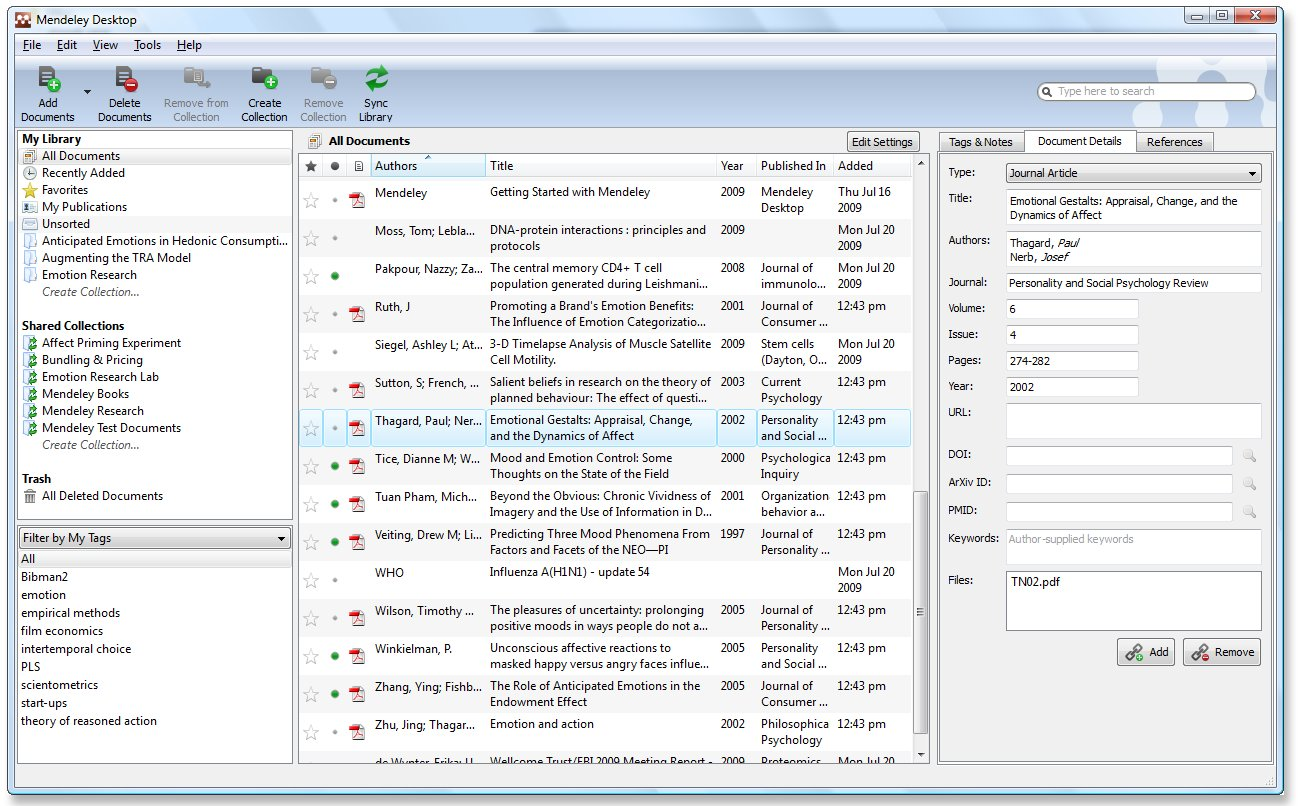
\includegraphics[width=1\textwidth]{img/Mendeley-destop-screenshot}\\ % Pfad
\source{\url{http://dominique-fleury.com/?p=302}} % Quelle
\end{minipage}
\end{figure}

\subsection{Texteditor}

Als Texteditor für \LaTeX wird Sublime Text (\url{http://www.sublimetext.com}) empfohlen. Zur Arbeit mit Latex ist das Plugin \emph{LaTeXTools} erforderlich (\url{https://github.com/SublimeText/LaTeXTools}).

\begin{figure}[hbt]
\centering
\begin{minipage}[t]{1\textwidth} % Breite, z.B. 1\textwidth		
\caption{Sublime Texteditor} % Überschrift
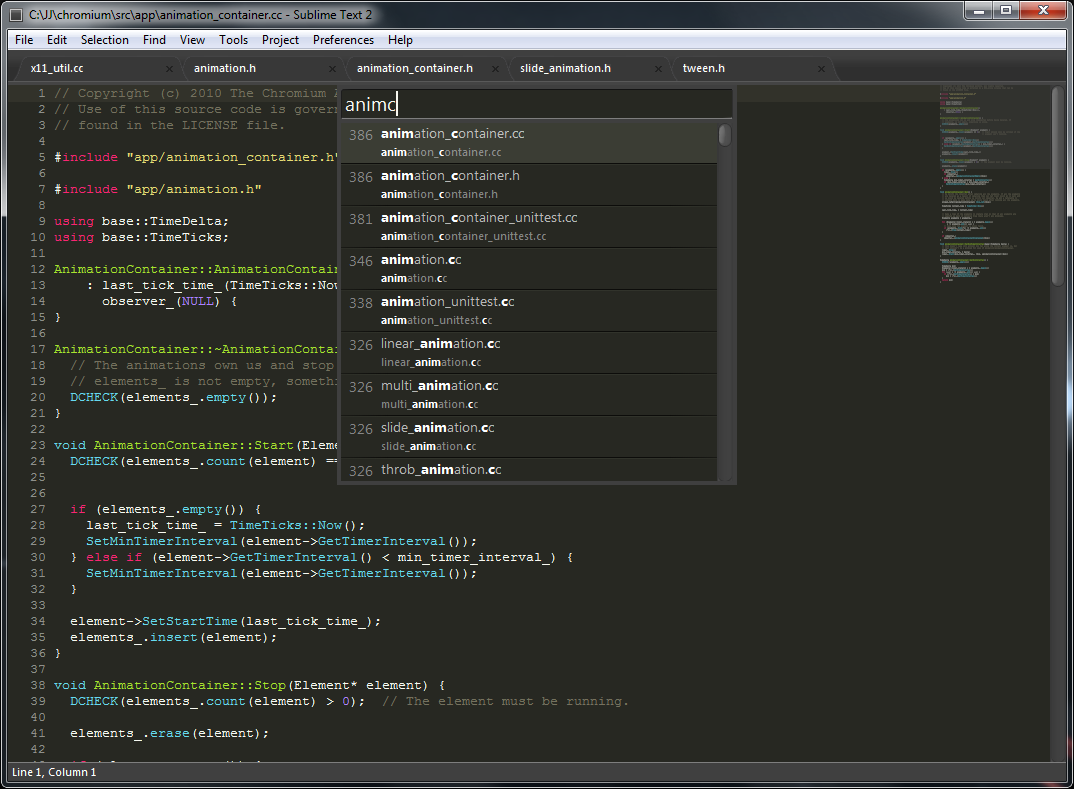
\includegraphics[width=1\textwidth]{img/sublime.png}\\ % Pfad
\source{\url{http://www.sublimetext.com/screenshots/alpha_goto_anything2_large.png}} % Quelle
\end{minipage}
\end{figure}

\subsection{PDF-Erzeugung}

Für die Erzeugung des PDF-Dokuments inklusive Referenzen, Quellenverzeichnis und Glossar sind mehrere Programmaufrufe und -durchläufe erforderlich. Der vollständige Aufruf zur PDF-Erzeugung lautet: 

\texttt{pdflatex Thesis}\\
\texttt{biber Thesis}\\
\texttt{makeindex -s Thesis.ist -t Thesis.alg -o Thesis.acr Thesis.acn}\\
\texttt{makeglossaries Thesis}\\
\texttt{pdflatex Thesis}\\
\texttt{pdflatex Thesis}\\

%!TEX root = ../Thesis.tex
\section{Grundlagen}

\subsection{Schrift}
\label{sec:schrift}

\subsubsection{Schriftgrößen}
\label{sec:schriftgroessen}
\tiny Das ist sehr kleine Schrift\\
\small Das ist kleine Schrift\\
\normalsize Das ist normale Schrift\\
\large Das ist große Schrift\\
\Large Das ist größere Schrift\\
\LARGE Das ist noch größere Schrift\\
\huge Das ist riesige Schrift\\
\Huge Das ist noch riesigere Schrift\\
\scriptsize Das ist Script Schrift\\
\footnotesize Das ist Fußnoten Schrift
\normalsize

\subsubsection{Schrift Typen}
\label{sec:Schrift Typen}
\textbf{Das ist ein fetter Text}\\
\textit{Das ist ein kursiver Text}\\
\underline{Das ist ein unterstrichener Text}\\
\textsc{Das ist ein kapitälchen Text}\\
\textsf{Das ist ein serifenloser Text}\\
\texttt{Das ist ein Schreibmaschinen Text}\\
\textnormal{Das ist ein normaler Text}

\subsubsection{Schrift Ausrichtung}
\label{sec:Schrift Ausrichtung}
\begin{quote}
Quote Text (Der gesamte Text innerhalb der Umgebung wird von beiden Seiten eingerückt)
\end{quote}
\begin{center}
Zentrierter Text (Der gesamte Text innerhalb der Umgebung wird zentriert)
\end{center}
\begin{flushleft}
Linksbündiger Text (Der gesamte Text innerhalb der Umgebung wird linksbündig)
\end{flushleft}
\begin{flushright}
Rechtsbündiger Text (Der gesamte Text innerhalb der Umgebung wird rechtsbündig)
\end{flushright}
In einer Fußnote\footnote{können zusätzliche Ergänzungen, Präzisierungen, Textverweise usw. eingeführt werden.}

\subsection{Abbildungen}

In \cref{fig:fhdw} sehen Sie das Logo der FHDW.

\begin{figure}[hbt]
\centering
\begin{minipage}[t]{.7\textwidth} % Breite, z.B. 1\textwidth		
\caption{Das Logo der FHDW} % Überschrift

\includegraphics[width=1\textwidth]{img/fhdw}\\ % Pfad
\source{Eigene Darstellung} % Quelle
\label{fig:fhdw}
\end{minipage}
\end{figure}

\subsection{Tabellen}

In \cref{tab:pin} auf Seite \pageref{tab:pin} sehen Sie die am häufigsten benutzten PINs.

\begin{table}[hbt]
\centering
\begin{minipage}[t]{.5\textwidth} % Breite, z.B. 1\textwidth		
\caption{Die am häufigsten verwendeten PINs} % Überschrift
\begin{tabularx}{\columnwidth}{rXrr}
\toprule
Rank & PIN & Percentage & Accumulated \\
\midrule
1 & 1234 & 4.34\% & 4.34\%\\
2 & 0000 & 2.57\% & 6.91\%\\
3 & 2580 & 2.32\% & 9.23\%\\
4 & 1111 & 1.60\% & 10.83\%\\
5 & 5555 & 0.87\% & 11.70\%\\
6 & 5683 & 0.70\% & 12.39\%\\
7 & 0852 & 0.60\% & 12.99\%\\
8 & 2222 & 0.56\% & 13.55\%\\
9 & 1212 & 0.49\% & 14.03\%\\
10 & 1998 & 0.43\% & 14.46\%\\
\bottomrule
\end{tabularx}
\source{Eigene Darstellung} % Quelle
\label{tab:pin}
\end{minipage}
\end{table}

\subsection{Zitate}

Ein Zitat im Fließtext ist zu sehen bei

Ein vergleichendes Zitat.\footnote{\cite[vgl.][5\psqq]{Maslennikov2011}}

Ein \enquote{wörtliches Zitat}\footnote{\cite[13\psq]{Meier2010}}

Zitat einer Quelle mit mehreren Autoren.\footnote{\cite[vgl.][32\psqq]{Hocking2011a}}


\subsection{Abkürzungen}
Bei der ersten Verwendung werden Abkürzungen ausgeschrieben: \gls{AES}.
Später wird dann automatisch nur noch die Kurzform benutzt: \gls{AES}


\subsection{Listen}
\label{sec:Listen}
Eine einfache List mit Punkten:

\begin{compactitem}
	\item Punkt 1
	\item Punkt 2
	\item Punkt 3
\end{compactitem}

Eine einfache Liste mit Nummern:
\begin{compactenum}
	\item Punkt 1
	\item Punkt 2 
	\item Punkt 3
\end{compactenum}

Eine einfache Liste mit römischen Nummern:
\begin{compactenum}[I.]
	\item Punkt 1
	\item Punkt 2
	\item Punkt 3
\end{compactenum}

Eine einfache Liste mit Buchstaben:
\begin{compactenum}[(a)]
	\item Punkt 1
	\item Punkt 2 
	\item Punkt 3
\end{compactenum}

\subsection{Quelltext}

Listing~\ref{list:android} auf Seite~\pageref{list:android} zeigt einigen Quelltext.

\begin{figure}[bht]
\begin{lstlisting}[caption=Scanning for Wi-Fi Access Points on Android, label=list:android]
registerReceiver(new RSSIBroadcastReceiver(), 
    new IntentFilter(WifiManager.SCAN_RESULTS_AVAILABLE_ACTION));

WifiManager wifi = getSystemService(Context.WIFI_SERVICE);
wifi.startScan();

/* not thread safe */
public class RSSIBroadcastReceiver extends BroadcastReceiver {

    public void onReceive(Context context, Intent intent) {
        WifiManager wifi = getSystemService(Context.WIFI_SERVICE);
        List<ScanResult> scanResults = wifiManager.getScanResults();

        for (ScanResult scanResult : results) {
            RSSI rssi = new RSSI();
            rssi.bssi = scanResult.BSSID;
            rssi.signalLevel = scanResult.level;
        }
    }
}
\end{lstlisting}
%\footnoterule{}
%\footnotesize{Casts have been omitted for the sake of readability}
\end{figure}

%!TEX root = ../Thesis.tex
\section{Zusammenfassung}

Dieses Dokument ist eine Hilfe, um die Formalien für eine Bachelor-Thesis an der
FHDW bei der Verwendung von {\LaTeX} zu erfüllen und dabei möglichst viele Automatismen von {\LaTeX} zu nutzen. Eine Absprache mit dem betreuenden Professor ist dennoch ratsam.

	
%%%%%%%%%%%%%%%%%%%%%%%%%%%%%%%%%%%%%%%%%%%%%%%%%%%%%%%%%%%%%%%%%%%%%%%

\end{document}